 \newcommand{\mypapersize}{A4}

\newcommand{\mylaterality}{twoside}

\newcommand{\mydraft}{false}

\newcommand{\myparskip}{half}

\newcommand{\myBCOR}{0mm}

\newcommand{\myfontsize}{12pt}

\newcommand{\mylinespread}{1.0}

\newcommand{\mylanguage}{ngerman,american}

\newcommand{\mybiblatexstyle}{authoryear}

\newcommand{\mybiblatexdashed}{false}  

\newcommand{\mybiblatexbackref}{true} 

%\newcommand{\mybiblatexfile}{references-biblatex.bib}

\newcommand{\mydispositioncolor}{0,0,0}

\newcommand{\mycolorlinks}{true} 

\newcommand{\mytitlepage}{template/title_Thesis_TU_Graz}

\newcommand{\mytodonotesoptions}{}

\documentclass[%
fontsize=\myfontsize,
paper=\mypapersize,  
parskip=\myparskip,  
DIV=calc,         
characters/line is great
headinclude=true,    
footinclude=false,  
open=right,          
appendixprefix=true, 
bibliography=totoc,  
draft=\mydraft,      
BCOR=\myBCOR,        
\mylaterality    
]{scrbook}  

\usepackage[utf8]{inputenc} 

\usepackage[\mylanguage]{babel}  

\usepackage{scrpage2} 

%\usepackage[backend=biber, 
%style=\mybiblatexstyle, 
%dashed=\mybiblatexdashed, 
%backref=\mybiblatexbackref, 
%natbib=true, 
%hyperref=true,
%]{biblatex}

%\addbibresource{\mybiblatexfile}
%\usepackage[numbers]{natbib}

\usepackage[pdftex]{graphicx}

\usepackage{pifont}

\usepackage{ifthen}

\newboolean{myaddcolophon}

\newboolean{myaddlistoftodos}

\usepackage{xspace}

\usepackage[usenames,dvipsnames]{xcolor}

\definecolor{DispositionColor}{RGB}{\mydispositioncolor}

\usepackage[normalem]{ulem}

\usepackage{framed}

\usepackage{eso-pic}

\usepackage{enumitem}

\usepackage[\mytodonotesoptions]{todonotes}  

\usepackage{units}

\usepackage{amsmath}

\usepackage[all]{xy}

\usepackage{amsthm}

\usepackage{float}

\usepackage{graphicx}

\usepackage{mathrsfs}

\usepackage{caption}

\usepackage{subcaption}

\usepackage{thmtools}

\usepackage{
nameref,
hyperref,
cleveref,
}

\usepackage{verbatim}

\usepackage{tabularx}

\usepackage{color}

\usepackage{amssymb}

\usepackage{setspace}

\usepackage{algpseudocode}

\usepackage{algorithm}

\usepackage{mathtools}

\usepackage{listings}

\usepackage{booktabs}

\usepackage[export]{adjustbox}%% DO NOT REMOVE THIS LINE!

\setboolean{myaddcolophon}{false}

\setboolean{myaddlistoftodos}{false}  

%% ========================================================================
%%%% Document metadata
%% ========================================================================

%% general metadata:
\newcommand{\myauthor}{Clemens Andritsch}
\newcommand{\mytitle}{Comparing Trees} 

\newcommand{\myworktitle}{Master's Thesis}  
\newcommand{\mygrade}{Bachelor of Science}
\newcommand{\mystudy}{Mathematik}
\newcommand{\myuniversity}{Graz University of Technology}
\newcommand{\myinstitute}{Institute for Discrete Mathematics}
\newcommand{\myinstitutehead}{Univ.-Prof. Dipl.-Ing. Dr.rer.nat. Woess Wolfgang} 
\newcommand{\mysupervisor}{Ao.Univ.-Prof. Dipl.-Ing. Dr.techn. Dragoti-Cela Eranda}
\newcommand{\myhomestreet}{Franckstraße 35 / 6} 
\newcommand{\myhometown}{Graz}
\newcommand{\myhomepostalnumber}{8010} 
\newcommand{\mysubmissionmonth}{July} 
\newcommand{\mysubmissionyear}{2020} 
\newcommand{\mysubmissiontown}{\myhometown} 

\newcommand{\myid}{01330358} 
\newcommand{\mylecture}{Graph Theory} 


%% Time-stamp: <2015-04-30 17:19:58 vk>
%%%% === Disclaimer: =======================================================
%% created by
%%
%%      Karl Voit
%%
%% using GNU/Linux, GNU Emacs & LaTeX 2e
%%

%doc%
%doc% \section{\texttt{mycommands.tex} --- various definitions}\myinteresting
%doc% \label{sec:mycommands}
%doc%
%doc% In file \verb#template/mycommands.tex# many useful commands are being
%doc% defined. 
%doc% 
%doc% \paragraph{What should I do with this file?} Please take a look at its 
%doc% content to get the most out of your document.
%doc% 

%doc% 
%doc% One of the best advantages of \LaTeX{} compared to \myacro{WYSIWYG} software products is
%doc% the possibility to define and use macros within text. This empowers the user to
%doc% a great extend.  Many things can be defined using \verb#\newcommand{}# and
%doc% automates repeating tasks. It is recommended to use macros not only for
%doc% repetitive tasks but also for separating form from content such as \myacro{CSS}
%doc% does for \myacro{XHTML}. Think of including graphics in your document: after
%doc% writing your book, you might want to change all captions to the upper side of
%doc% each figure. In this case you either have to modify all
%doc% \texttt{includegraphics} commands or you were clever enough to define something
%doc% like \verb#\myfig#\footnote{See below for a detailed description}. Using a
%doc% macro for including graphics enables you to modify the position caption on only
%doc% \emph{one} place: at the definition of the macro.
%doc% 
%doc% The following section describes some macros that came with this document template
%doc% from \myLaT and you are welcome to modify or extend them or to create
%doc% your own macros!
%doc% 

%doc% 
%doc% \subsection{\texttt{myfig} --- including graphics made easy}
%doc% 
%doc% The classic: you can easily add graphics to your document with \verb#\myfig#:
%doc% \begin{verbatim}
%doc%  \myfig{flower}%% filename w/o extension in the folder figures
%doc%        {width=0.7\textwidth}%% maximum width/height, aspect ratio will be kept
%doc%        {This flower was photographed at my home town in 2010}%% caption
%doc%        {Home town flower}%% optional (short) caption for list of figures
%doc%        {fig:flower}%% label
%doc% \end{verbatim}
%doc% 
%doc% There are many advantages of this command (compared to manual
%doc% \texttt{figure} environments and \texttt{includegraphics} commands:
%doc% \begin{itemize}
%doc% \item consistent style throughout the whole document
%doc% \item easy to change; for example move caption on top
%doc% \item much less characters to type (faster, error prone)
%doc% \item less visual clutter in the \TeX{}-files
%doc% \end{itemize}
%doc% 
%doc% 
\newcommand{\myfig}[5]{
%% example:
% \myfig{}%% filename in figures folder
%       {width=0.5\textwidth,height=0.5\textheight}%% maximum width/height, aspect ratio will be kept
%       {}%% caption
%       {}%% optional (short) caption for list of figures
%       {}%% label
\begin{figure}%[htp]
  \centering
  \includegraphics[keepaspectratio,#2]{figures/#1}
  \caption[#4]{#3}
  \label{#5} %% NOTE: always label *after* caption!
\end{figure}
}


%doc% 
%doc% \subsection{\texttt{myclone} --- repeat things!}
%doc% 
%doc% Using \verb#\myclone[42]{foobar}# results the text \enquote{foobar} printed 42 times.
%doc% But you can not only repeat text output with \texttt{myclone}. 
%doc%
%doc% Default argument
%doc% for the optional parameter \enquote{number of times} (like \enquote{42} in the example above) 
%doc% is set to two.
%doc% 
%% \myclone[x]{text}
\newcounter{myclonecnt}
\newcommand{\myclone}[2][2]{%
  \setcounter{myclonecnt}{#1}%
  \whiledo{\value{myclonecnt}>0}{#2\addtocounter{myclonecnt}{-1}}%
}

%old% %d oc% 
%old% %d oc% \subsection{\texttt{fixxme} --- sidemark something as unfinished}
%old% %d oc% 
%old% %d oc% You know it: something has to be fixed and you can not do it right
%old% %d oc% now. In order to \texttt{not} forget about it, you might want to add a
%old% %d oc% note like \verb+\fixxme{check again}+ which inserts a note on the page
%old% %d oc% margin such as this\fixxme{check again} example.
%old% %d oc%
%old% \newcommand{\fixxme}[1]{%%
%old% \textcolor{red}{FIXXME}\marginpar{\textcolor{red}{#1}}%%
%old% }


%%%% End 
%%% Local Variables:
%%% mode: latex
%%% mode: auto-fill
%%% mode: flyspell
%%% eval: (ispell-change-dictionary "en_US")
%%% TeX-master: "../main"
%%% End:
%% vim:foldmethod=expr
%% vim:fde=getline(v\:lnum)=~'^%%%%'?0\:getline(v\:lnum)=~'^%doc.*\ .\\%(sub\\)\\?section{.\\+'?'>1'\:'1':


%%%% Time-stamp: <2015-08-22 17:20:32 vk>
%%%% === Disclaimer: =======================================================
%% created by
%%
%%      Karl Voit
%%
%% using GNU/Linux, GNU Emacs & LaTeX 2e
%%
%doc%
%doc% \section{\texttt{typographic\_settings.tex} --- Typographic finetuning}
%doc%
%doc% The settings of file \verb#template/typographic_settings.tex# contain
%doc% typographic finetuning related to things mentioned in literature.  The
%doc% settings in this file relates to personal taste and most of all: 
%doc% \emph{typographic experience}. 
%doc% 
%doc% \paragraph{What should I do with this file?} You might as well skip the whole
%doc% file by excluding the \verb#%%%% Time-stamp: <2015-08-22 17:20:32 vk>
%%%% === Disclaimer: =======================================================
%% created by
%%
%%      Karl Voit
%%
%% using GNU/Linux, GNU Emacs & LaTeX 2e
%%
%doc%
%doc% \section{\texttt{typographic\_settings.tex} --- Typographic finetuning}
%doc%
%doc% The settings of file \verb#template/typographic_settings.tex# contain
%doc% typographic finetuning related to things mentioned in literature.  The
%doc% settings in this file relates to personal taste and most of all: 
%doc% \emph{typographic experience}. 
%doc% 
%doc% \paragraph{What should I do with this file?} You might as well skip the whole
%doc% file by excluding the \verb#%%%% Time-stamp: <2015-08-22 17:20:32 vk>
%%%% === Disclaimer: =======================================================
%% created by
%%
%%      Karl Voit
%%
%% using GNU/Linux, GNU Emacs & LaTeX 2e
%%
%doc%
%doc% \section{\texttt{typographic\_settings.tex} --- Typographic finetuning}
%doc%
%doc% The settings of file \verb#template/typographic_settings.tex# contain
%doc% typographic finetuning related to things mentioned in literature.  The
%doc% settings in this file relates to personal taste and most of all: 
%doc% \emph{typographic experience}. 
%doc% 
%doc% \paragraph{What should I do with this file?} You might as well skip the whole
%doc% file by excluding the \verb#\input{template/typographic_settings.tex}# command
%doc% in \texttt{main.tex}.  For standard usage it is recommended to stay with the
%doc% default settings.
%doc% 
%doc% 
%% ========================================================================

%doc%
%doc% Some basic microtypographic settings are provided by the
%doc% \texttt{microtype}
%doc% package\footnote{\url{http://ctan.org/pkg/microtype}}. This template
%doc% uses the rather conservative package parameters: \texttt{protrusion=true,factor=900}.
\usepackage[protrusion=true,factor=900]{microtype}

%doc%
%doc% \subsection{French spacing}
%doc%
%doc% \paragraph{Why?} see~\textcite[p.\,28, p.\,30]{Bringhurst1993}: `2.1.4 Use a single word space between sentences.'
%doc%
%doc% \paragraph{How?} see~\textcite[p.\,185]{Eijkhout2008}:\\
%doc% \verb#\frenchspacing  %% Macro to switch off extra space after punctuation.# \\
\frenchspacing  %% Macro to switch off extra space after punctuation.
%doc%
%doc% Note: This setting might be default for \myacro{KOMA} script.
%doc%


%doc%
%doc% \subsection{Font}
%doc% 
%doc% This template is using the Palatino font (package \texttt{mathpazo}) which results
%doc% in a legible document and matching mathematical fonts for printout.
%doc% 
%doc% It is highly recommended that you either stick to the Palatino font or use the
%doc% \LaTeX{} default fonts (by removing the package \texttt{mathpazo}).
%doc% 
%doc% Chosing different fonts is not
%doc% an easy task. Please leave this to people with good knowledge on this subject.
%doc% 
%doc% One valid reason to change the default fonts is when your document is mainly
%doc% read on a computer screen. In this case it is recommended to switch to a font
%doc% \textsf{which is sans-serif like this}. This template contains several alternative
%doc% font packages which can be activated in this file.
%doc% 

% for changing the default font, please go to the next subsection!

%doc%
%doc% \subsection{Text figures}
%doc% 
%doc% \ldots also called old style numbers such as 0123456789. 
%doc% (German: \enquote{Mediäval\-ziffern\footnote{\url{https://secure.wikimedia.org/wikibooks/de/wiki/LaTeX-W\%C3\%B6rterbuch:\_Medi\%C3\%A4valziffern}}})
%doc% \paragraph{Why?} see~\textcite[p.\,44f]{Bringhurst1993}: 
%doc% \begin{quote}
%doc% `3.2.1 If the font includes both text figures and titling figures, use
%doc%  titling figures only with full caps, and text figures in all other
%doc%  circumstances.'
%doc% \end{quote}
%doc% 
%doc% \paragraph{How?} 
%doc% Quoted from Wikibooks\footnote{\url{https://secure.wikimedia.org/wikibooks/en/wiki/LaTeX/Formatting\#Text\_figures\_.28.22old\_style.22\_numerals.29}}:
%doc% \begin{quote}
%doc% Some fonts do not have text figures built in; the textcomp package attempts to
%doc% remedy this by effectively generating text figures from the currently-selected
%doc% font. Put \verb#\usepackage{textcomp}# in your preamble. textcomp also allows you to
%doc% use decimal points, properly formatted dollar signs, etc. within
%doc% \verb#\oldstylenums{}#.
%doc% \end{quote}
%doc% \ldots but proposed \LaTeX{} method does not work out well. Instead use:\\
%doc% \verb#\usepackage{hfoldsty}#  (enables text figures using additional font) or \\
%doc% \verb#\usepackage[sc,osf]{mathpazo}# (switches to Palatino font with small caps and old style figures enabled).
%doc%
%\usepackage{hfoldsty}  %% enables text figures using additional font
%% ... OR use ...
\usepackage[sc,osf]{mathpazo} %% switches to Palatino with small caps and old style figures

%% Font selection from:
%%     http://www.matthiaspospiech.de/latex/vorlagen/allgemein/preambel/fonts/
%% use following lines *instead* of the mathpazo package above:
%% ===== Serif =========================================================
%% for Computer Modern (LaTeX default font), simply remove the mathpazo above
%\usepackage{charter}\linespread{1.05} %% Charter
%\usepackage{bookman}                  %% Bookman (laedt Avant Garde !!)
%\usepackage{newcent}                  %% New Century Schoolbook (laedt Avant Garde !!)
%% ===== Sans Serif ====================================================
%\renewcommand{\familydefault}{\sfdefault}  %% this one in *combination* with the default mathpazo package
%\usepackage{cmbright}                  %% CM-Bright (eigntlich eine Familie)
%\usepackage{tpslifonts}                %% tpslifonts % Font for Slides


%doc% 
%doc% \subsection{\texttt{myacro} --- Abbrevations using \textsc{small caps}}\myinteresting
%doc% \label{sec:myacro}
%doc% 
%doc% \paragraph{Why?} see~\textcite[p.\,45f]{Bringhurst1993}: `3.2.2 For abbrevations and
%doc% acronyms in the midst of normal text, use spaced small caps.'
%doc% 
%doc% \paragraph{How?} Using the predefined macro \verb#\myacro{}# for things like
%doc% \myacro{UNO} or \myacro{UNESCO} using \verb#\myacro{UNO}# or \verb#\myacro{UNESCO}#.
%doc% 
\DeclareRobustCommand{\myacro}[1]{\textsc{\lowercase{#1}}} %%  abbrevations using small caps


%doc% 
%doc% \subsection{Colorized headings and links}
%doc% 
%doc% This document template is able to generate an output that uses colorized
%doc% headings, captions, page numbers, and links. The color named `DispositionColor'
%doc% used in this document is defined near the definition of package \texttt{color}
%doc% in the preamble (see section~\ref{subsec:miscpackages}). The changes required
%doc% for headings, page numbers, and captions are defined here.
%doc% 
%doc% Settings for colored links are handled by the definitions of the
%doc% \texttt{hyperref} package (see section~\ref{sec:pdf}).
%doc% 
\setheadsepline{.4pt}[\color{DispositionColor}]
\renewcommand{\headfont}{\normalfont\sffamily\color{DispositionColor}}
\renewcommand{\pnumfont}{\normalfont\sffamily\color{DispositionColor}}
\addtokomafont{disposition}{\color{DispositionColor}}
\addtokomafont{caption}{\color{DispositionColor}\footnotesize}
\addtokomafont{captionlabel}{\color{DispositionColor}}

%doc% 
%doc% \subsection{No figures or tables below footnotes}
%doc% 
%doc% \LaTeX{} places floating environments below footnotes if \texttt{b}
%doc% (bottom) is used as (default) placement algorithm. This is certainly
%doc% not appealing for most people and is deactivated in this template by
%doc% using the package \texttt{footmisc} with its option \texttt{bottom}.
%doc% 
%% see also: http://www.komascript.de/node/858 (German description)
\usepackage[bottom]{footmisc}

%doc% 
%doc% \subsection{Spacings of list environments}
%doc% 
%doc% By default, \LaTeX{} is using vertical spaces between items of enumerate, 
%doc% itemize and description environments. This is fine for multi-line items.
%doc% Many times, the user does just write single-line items where the larger
%doc% vertical space is inappropriate. The \href{http://ctan.org/pkg/enumitem}{enumitem}
%doc% package provides replacements for the pre-defined list environments and
%doc% offers many options to modify their appearances.
%doc% This template is using the package option for \texttt{noitemsep} which
%doc% mimimizes the vertical space between list items.
%doc% 
\usepackage{enumitem}
\setlist{noitemsep}   %% kills the space between items

%doc% 
%doc% \subsection{\texttt{csquotes} --- Correct quotation marks}\myinteresting
%doc% \label{sub:csquotes}
%doc% 
%doc% \emph{Never} use quotation marks found on your keyboard.
%doc% They end up in strange characters or false looking quotation marks.
%doc% 
%doc% In \LaTeX{} you are able to use typographically correct quotation marks. The package 
%doc% \href{http://www.ctan.org/pkg/csquotes}{\texttt{csquotes}} offers you with 
%doc% \verb#\enquote{foobar}# a command to get correct quotation marks around \enquote{foobar}.
%doc% Please do check the package options in order to modify
%doc% its settings according to the language used\footnote{most of the time in 
%doc% combination with the language set in the options of the \texttt{babel} package}.
%doc% 
%doc% \href{http://www.ctan.org/pkg/csquotes}{\texttt{csquotes}} is also recommended 
%doc% by \texttt{biblatex} (see Section~\ref{sec:references}). 
\usepackage[babel=true,strict=true,english=american,german=guillemets]{csquotes}

%doc% 
%doc% \subsection{Line spread}
%doc% 
%doc% If you have to enlarge the distance between two lines of text, you can
%doc% increase it using the \texttt{\mylinespread} command in \texttt{main.tex}. By default, it is
%doc% deactivated (set to 100~percent). Modify only with caution since it influences the
%doc% page layout and could lead to ugly looking documents.
\linespread{\mylinespread}

%doc% 
%doc% \subsection{Optional: Lines above and below the chapter head}
%doc% 
%doc% This is not quite something typographic but rather a matter of taste.
%doc% \myacro{KOMA} Script offers \href{http://www.komascript.de/node/24}{a method to
%doc% add lines above and below chapter head} which is disabled by
%doc% default. If you want to enable this feature, remove corresponding
%doc% comment characters from the settings.
%doc% 
%% Source: http://www.komascript.de/node/24
%disabled% %% 1st get a new command
%disabled% \newcommand*{\ORIGchapterheadstartvskip}{}%
%disabled% %% 2nd save the original definition to the new command
%disabled% \let\ORIGchapterheadstartvskip=\chapterheadstartvskip
%disabled% %% 3rd redefine the command using the saved original command
%disabled% \renewcommand*{\chapterheadstartvskip}{%
%disabled%   \ORIGchapterheadstartvskip
%disabled%   {%
%disabled%     \setlength{\parskip}{0pt}%
%disabled%     \noindent\color{DispositionColor}\rule[.3\baselineskip]{\linewidth}{1pt}\par
%disabled%   }%
%disabled% }
%disabled% %% see above
%disabled% \newcommand*{\ORIGchapterheadendvskip}{}%
%disabled% \let\ORIGchapterheadendvskip=\chapterheadendvskip
%disabled% \renewcommand*{\chapterheadendvskip}{%
%disabled%   {%
%disabled%     \setlength{\parskip}{0pt}%
%disabled%     \noindent\color{DispositionColor}\rule[.3\baselineskip]{\linewidth}{1pt}\par
%disabled%   }%
%disabled%   \ORIGchapterheadendvskip
%disabled% }

%doc% 
%doc% \subsection{Optional: Chapter thumbs}
%doc% 
%doc% This is not quite something typographic but rather a matter of taste.
%doc% \myacro{KOMA} Script offers \href{http://www.komascript.de/chapterthumbs-example}{a method to
%doc% add chapter thumbs} (in combination with the package \texttt{scrpage2}) which is disabled by
%doc% default. If you want to enable this feature, remove corresponding
%doc% comment characters from the settings.
%doc% 
%disabled% \makeatletter
%disabled% % Safty first
%disabled% \@ifundefined{chapter}{\let\chapter\undefined
%disabled%   \chapter must be defined to use chapter thumbs!}{%
%disabled%  
%disabled% % Two new commands for the width and height of the boxes with the
%disabled% % chapter number at the thumbs (use of commands instead of lengths
%disabled% % for sparing registers)
%disabled% \newcommand*{\chapterthumbwidth}{2em}
%disabled% \newcommand*{\chapterthumbheight}{1em}
%disabled%  
%disabled% % Two new commands for the colors of the box background and the
%disabled% % chapter numbers of the thumbs
%disabled% \newcommand*{\chapterthumbboxcolor}{black}
%disabled% \newcommand*{\chapterthumbtextcolor}{white}
%disabled%  
%disabled% % New command to set a chapter thumb. I'm using a group at this
%disabled% % command, because I'm changing the temporary dimension \@tempdima
%disabled% \newcommand*{\putchapterthumb}{%
%disabled%   \begingroup
%disabled%     \Large
%disabled%     % calculate the horizontal possition of the right paper border
%disabled%     % (I ignore \hoffset, because I interprete \hoffset moves the page
%disabled%     % at the paper e.g. if you are using cropmarks)
%disabled%     \setlength{\@tempdima}{\@oddheadshift}% (internal from scrpage2)
%disabled%     \setlength{\@tempdima}{-\@tempdima}%
%disabled%     \addtolength{\@tempdima}{\paperwidth}%
%disabled%     \addtolength{\@tempdima}{-\oddsidemargin}%
%disabled%     \addtolength{\@tempdima}{-1in}%
%disabled%     % putting the thumbs should not change the horizontal
%disabled%     % possition
%disabled%     \rlap{%
%disabled%       % move to the calculated horizontal possition
%disabled%       \hspace*{\@tempdima}%
%disabled%       % putting the thumbs should not change the vertical
%disabled%       % possition
%disabled%       \vbox to 0pt{%
%disabled%         % calculate the vertical possition of the thumbs (I ignore
%disabled%         % \voffset for the same reasons told above)
%disabled%         \setlength{\@tempdima}{\chapterthumbwidth}%
%disabled%         \multiply\@tempdima by\value{chapter}%
%disabled%         \addtolength{\@tempdima}{-\chapterthumbwidth}%
%disabled%         \addtolength{\@tempdima}{-\baselineskip}%
%disabled%         % move to the calculated vertical possition
%disabled%         \vspace*{\@tempdima}%
%disabled%         % put the thumbs left so the current horizontal possition
%disabled%         \llap{%
%disabled%           % and rotate them
%disabled%           \rotatebox{90}{\colorbox{\chapterthumbboxcolor}{%
%disabled%               \parbox[c][\chapterthumbheight][c]{\chapterthumbwidth}{%
%disabled%                 \centering
%disabled%                 \textcolor{\chapterthumbtextcolor}{%
%disabled%                   \strut\thechapter}\\
%disabled%               }%
%disabled%             }%
%disabled%           }%
%disabled%         }%
%disabled%         % avoid overfull \vbox messages
%disabled%         \vss
%disabled%       }%
%disabled%     }%
%disabled%   \endgroup
%disabled% }
%disabled%  
%disabled% % New command, which works like \lohead but also puts the thumbs (you
%disabled% % cannot use \ihead with this definition but you may change this, if
%disabled% % you use more internal scrpage2 commands)
%disabled% \newcommand*{\loheadwithchapterthumbs}[2][]{%
%disabled%   \lohead[\putchapterthumb#1]{\putchapterthumb#2}%
%disabled% }
%disabled%  
%disabled% % initial use
%disabled% \loheadwithchapterthumbs{}
%disabled% \pagestyle{scrheadings}
%disabled%  
%disabled% }
%disabled% \makeatother

%%%% END
%%% Local Variables:
%%% mode: latex
%%% mode: auto-fill
%%% mode: flyspell
%%% eval: (ispell-change-dictionary "en_US")
%%% TeX-master: "../main"
%%% End:
%% vim:foldmethod=expr
%% vim:fde=getline(v\:lnum)=~'^%%%%'?0\:getline(v\:lnum)=~'^%doc.*\ .\\%(sub\\)\\?section{.\\+'?'>1'\:'1':
# command
%doc% in \texttt{main.tex}.  For standard usage it is recommended to stay with the
%doc% default settings.
%doc% 
%doc% 
%% ========================================================================

%doc%
%doc% Some basic microtypographic settings are provided by the
%doc% \texttt{microtype}
%doc% package\footnote{\url{http://ctan.org/pkg/microtype}}. This template
%doc% uses the rather conservative package parameters: \texttt{protrusion=true,factor=900}.
\usepackage[protrusion=true,factor=900]{microtype}

%doc%
%doc% \subsection{French spacing}
%doc%
%doc% \paragraph{Why?} see~\textcite[p.\,28, p.\,30]{Bringhurst1993}: `2.1.4 Use a single word space between sentences.'
%doc%
%doc% \paragraph{How?} see~\textcite[p.\,185]{Eijkhout2008}:\\
%doc% \verb#\frenchspacing  %% Macro to switch off extra space after punctuation.# \\
\frenchspacing  %% Macro to switch off extra space after punctuation.
%doc%
%doc% Note: This setting might be default for \myacro{KOMA} script.
%doc%


%doc%
%doc% \subsection{Font}
%doc% 
%doc% This template is using the Palatino font (package \texttt{mathpazo}) which results
%doc% in a legible document and matching mathematical fonts for printout.
%doc% 
%doc% It is highly recommended that you either stick to the Palatino font or use the
%doc% \LaTeX{} default fonts (by removing the package \texttt{mathpazo}).
%doc% 
%doc% Chosing different fonts is not
%doc% an easy task. Please leave this to people with good knowledge on this subject.
%doc% 
%doc% One valid reason to change the default fonts is when your document is mainly
%doc% read on a computer screen. In this case it is recommended to switch to a font
%doc% \textsf{which is sans-serif like this}. This template contains several alternative
%doc% font packages which can be activated in this file.
%doc% 

% for changing the default font, please go to the next subsection!

%doc%
%doc% \subsection{Text figures}
%doc% 
%doc% \ldots also called old style numbers such as 0123456789. 
%doc% (German: \enquote{Mediäval\-ziffern\footnote{\url{https://secure.wikimedia.org/wikibooks/de/wiki/LaTeX-W\%C3\%B6rterbuch:\_Medi\%C3\%A4valziffern}}})
%doc% \paragraph{Why?} see~\textcite[p.\,44f]{Bringhurst1993}: 
%doc% \begin{quote}
%doc% `3.2.1 If the font includes both text figures and titling figures, use
%doc%  titling figures only with full caps, and text figures in all other
%doc%  circumstances.'
%doc% \end{quote}
%doc% 
%doc% \paragraph{How?} 
%doc% Quoted from Wikibooks\footnote{\url{https://secure.wikimedia.org/wikibooks/en/wiki/LaTeX/Formatting\#Text\_figures\_.28.22old\_style.22\_numerals.29}}:
%doc% \begin{quote}
%doc% Some fonts do not have text figures built in; the textcomp package attempts to
%doc% remedy this by effectively generating text figures from the currently-selected
%doc% font. Put \verb#\usepackage{textcomp}# in your preamble. textcomp also allows you to
%doc% use decimal points, properly formatted dollar signs, etc. within
%doc% \verb#\oldstylenums{}#.
%doc% \end{quote}
%doc% \ldots but proposed \LaTeX{} method does not work out well. Instead use:\\
%doc% \verb#\usepackage{hfoldsty}#  (enables text figures using additional font) or \\
%doc% \verb#\usepackage[sc,osf]{mathpazo}# (switches to Palatino font with small caps and old style figures enabled).
%doc%
%\usepackage{hfoldsty}  %% enables text figures using additional font
%% ... OR use ...
\usepackage[sc,osf]{mathpazo} %% switches to Palatino with small caps and old style figures

%% Font selection from:
%%     http://www.matthiaspospiech.de/latex/vorlagen/allgemein/preambel/fonts/
%% use following lines *instead* of the mathpazo package above:
%% ===== Serif =========================================================
%% for Computer Modern (LaTeX default font), simply remove the mathpazo above
%\usepackage{charter}\linespread{1.05} %% Charter
%\usepackage{bookman}                  %% Bookman (laedt Avant Garde !!)
%\usepackage{newcent}                  %% New Century Schoolbook (laedt Avant Garde !!)
%% ===== Sans Serif ====================================================
%\renewcommand{\familydefault}{\sfdefault}  %% this one in *combination* with the default mathpazo package
%\usepackage{cmbright}                  %% CM-Bright (eigntlich eine Familie)
%\usepackage{tpslifonts}                %% tpslifonts % Font for Slides


%doc% 
%doc% \subsection{\texttt{myacro} --- Abbrevations using \textsc{small caps}}\myinteresting
%doc% \label{sec:myacro}
%doc% 
%doc% \paragraph{Why?} see~\textcite[p.\,45f]{Bringhurst1993}: `3.2.2 For abbrevations and
%doc% acronyms in the midst of normal text, use spaced small caps.'
%doc% 
%doc% \paragraph{How?} Using the predefined macro \verb#\myacro{}# for things like
%doc% \myacro{UNO} or \myacro{UNESCO} using \verb#\myacro{UNO}# or \verb#\myacro{UNESCO}#.
%doc% 
\DeclareRobustCommand{\myacro}[1]{\textsc{\lowercase{#1}}} %%  abbrevations using small caps


%doc% 
%doc% \subsection{Colorized headings and links}
%doc% 
%doc% This document template is able to generate an output that uses colorized
%doc% headings, captions, page numbers, and links. The color named `DispositionColor'
%doc% used in this document is defined near the definition of package \texttt{color}
%doc% in the preamble (see section~\ref{subsec:miscpackages}). The changes required
%doc% for headings, page numbers, and captions are defined here.
%doc% 
%doc% Settings for colored links are handled by the definitions of the
%doc% \texttt{hyperref} package (see section~\ref{sec:pdf}).
%doc% 
\setheadsepline{.4pt}[\color{DispositionColor}]
\renewcommand{\headfont}{\normalfont\sffamily\color{DispositionColor}}
\renewcommand{\pnumfont}{\normalfont\sffamily\color{DispositionColor}}
\addtokomafont{disposition}{\color{DispositionColor}}
\addtokomafont{caption}{\color{DispositionColor}\footnotesize}
\addtokomafont{captionlabel}{\color{DispositionColor}}

%doc% 
%doc% \subsection{No figures or tables below footnotes}
%doc% 
%doc% \LaTeX{} places floating environments below footnotes if \texttt{b}
%doc% (bottom) is used as (default) placement algorithm. This is certainly
%doc% not appealing for most people and is deactivated in this template by
%doc% using the package \texttt{footmisc} with its option \texttt{bottom}.
%doc% 
%% see also: http://www.komascript.de/node/858 (German description)
\usepackage[bottom]{footmisc}

%doc% 
%doc% \subsection{Spacings of list environments}
%doc% 
%doc% By default, \LaTeX{} is using vertical spaces between items of enumerate, 
%doc% itemize and description environments. This is fine for multi-line items.
%doc% Many times, the user does just write single-line items where the larger
%doc% vertical space is inappropriate. The \href{http://ctan.org/pkg/enumitem}{enumitem}
%doc% package provides replacements for the pre-defined list environments and
%doc% offers many options to modify their appearances.
%doc% This template is using the package option for \texttt{noitemsep} which
%doc% mimimizes the vertical space between list items.
%doc% 
\usepackage{enumitem}
\setlist{noitemsep}   %% kills the space between items

%doc% 
%doc% \subsection{\texttt{csquotes} --- Correct quotation marks}\myinteresting
%doc% \label{sub:csquotes}
%doc% 
%doc% \emph{Never} use quotation marks found on your keyboard.
%doc% They end up in strange characters or false looking quotation marks.
%doc% 
%doc% In \LaTeX{} you are able to use typographically correct quotation marks. The package 
%doc% \href{http://www.ctan.org/pkg/csquotes}{\texttt{csquotes}} offers you with 
%doc% \verb#\enquote{foobar}# a command to get correct quotation marks around \enquote{foobar}.
%doc% Please do check the package options in order to modify
%doc% its settings according to the language used\footnote{most of the time in 
%doc% combination with the language set in the options of the \texttt{babel} package}.
%doc% 
%doc% \href{http://www.ctan.org/pkg/csquotes}{\texttt{csquotes}} is also recommended 
%doc% by \texttt{biblatex} (see Section~\ref{sec:references}). 
\usepackage[babel=true,strict=true,english=american,german=guillemets]{csquotes}

%doc% 
%doc% \subsection{Line spread}
%doc% 
%doc% If you have to enlarge the distance between two lines of text, you can
%doc% increase it using the \texttt{\mylinespread} command in \texttt{main.tex}. By default, it is
%doc% deactivated (set to 100~percent). Modify only with caution since it influences the
%doc% page layout and could lead to ugly looking documents.
\linespread{\mylinespread}

%doc% 
%doc% \subsection{Optional: Lines above and below the chapter head}
%doc% 
%doc% This is not quite something typographic but rather a matter of taste.
%doc% \myacro{KOMA} Script offers \href{http://www.komascript.de/node/24}{a method to
%doc% add lines above and below chapter head} which is disabled by
%doc% default. If you want to enable this feature, remove corresponding
%doc% comment characters from the settings.
%doc% 
%% Source: http://www.komascript.de/node/24
%disabled% %% 1st get a new command
%disabled% \newcommand*{\ORIGchapterheadstartvskip}{}%
%disabled% %% 2nd save the original definition to the new command
%disabled% \let\ORIGchapterheadstartvskip=\chapterheadstartvskip
%disabled% %% 3rd redefine the command using the saved original command
%disabled% \renewcommand*{\chapterheadstartvskip}{%
%disabled%   \ORIGchapterheadstartvskip
%disabled%   {%
%disabled%     \setlength{\parskip}{0pt}%
%disabled%     \noindent\color{DispositionColor}\rule[.3\baselineskip]{\linewidth}{1pt}\par
%disabled%   }%
%disabled% }
%disabled% %% see above
%disabled% \newcommand*{\ORIGchapterheadendvskip}{}%
%disabled% \let\ORIGchapterheadendvskip=\chapterheadendvskip
%disabled% \renewcommand*{\chapterheadendvskip}{%
%disabled%   {%
%disabled%     \setlength{\parskip}{0pt}%
%disabled%     \noindent\color{DispositionColor}\rule[.3\baselineskip]{\linewidth}{1pt}\par
%disabled%   }%
%disabled%   \ORIGchapterheadendvskip
%disabled% }

%doc% 
%doc% \subsection{Optional: Chapter thumbs}
%doc% 
%doc% This is not quite something typographic but rather a matter of taste.
%doc% \myacro{KOMA} Script offers \href{http://www.komascript.de/chapterthumbs-example}{a method to
%doc% add chapter thumbs} (in combination with the package \texttt{scrpage2}) which is disabled by
%doc% default. If you want to enable this feature, remove corresponding
%doc% comment characters from the settings.
%doc% 
%disabled% \makeatletter
%disabled% % Safty first
%disabled% \@ifundefined{chapter}{\let\chapter\undefined
%disabled%   \chapter must be defined to use chapter thumbs!}{%
%disabled%  
%disabled% % Two new commands for the width and height of the boxes with the
%disabled% % chapter number at the thumbs (use of commands instead of lengths
%disabled% % for sparing registers)
%disabled% \newcommand*{\chapterthumbwidth}{2em}
%disabled% \newcommand*{\chapterthumbheight}{1em}
%disabled%  
%disabled% % Two new commands for the colors of the box background and the
%disabled% % chapter numbers of the thumbs
%disabled% \newcommand*{\chapterthumbboxcolor}{black}
%disabled% \newcommand*{\chapterthumbtextcolor}{white}
%disabled%  
%disabled% % New command to set a chapter thumb. I'm using a group at this
%disabled% % command, because I'm changing the temporary dimension \@tempdima
%disabled% \newcommand*{\putchapterthumb}{%
%disabled%   \begingroup
%disabled%     \Large
%disabled%     % calculate the horizontal possition of the right paper border
%disabled%     % (I ignore \hoffset, because I interprete \hoffset moves the page
%disabled%     % at the paper e.g. if you are using cropmarks)
%disabled%     \setlength{\@tempdima}{\@oddheadshift}% (internal from scrpage2)
%disabled%     \setlength{\@tempdima}{-\@tempdima}%
%disabled%     \addtolength{\@tempdima}{\paperwidth}%
%disabled%     \addtolength{\@tempdima}{-\oddsidemargin}%
%disabled%     \addtolength{\@tempdima}{-1in}%
%disabled%     % putting the thumbs should not change the horizontal
%disabled%     % possition
%disabled%     \rlap{%
%disabled%       % move to the calculated horizontal possition
%disabled%       \hspace*{\@tempdima}%
%disabled%       % putting the thumbs should not change the vertical
%disabled%       % possition
%disabled%       \vbox to 0pt{%
%disabled%         % calculate the vertical possition of the thumbs (I ignore
%disabled%         % \voffset for the same reasons told above)
%disabled%         \setlength{\@tempdima}{\chapterthumbwidth}%
%disabled%         \multiply\@tempdima by\value{chapter}%
%disabled%         \addtolength{\@tempdima}{-\chapterthumbwidth}%
%disabled%         \addtolength{\@tempdima}{-\baselineskip}%
%disabled%         % move to the calculated vertical possition
%disabled%         \vspace*{\@tempdima}%
%disabled%         % put the thumbs left so the current horizontal possition
%disabled%         \llap{%
%disabled%           % and rotate them
%disabled%           \rotatebox{90}{\colorbox{\chapterthumbboxcolor}{%
%disabled%               \parbox[c][\chapterthumbheight][c]{\chapterthumbwidth}{%
%disabled%                 \centering
%disabled%                 \textcolor{\chapterthumbtextcolor}{%
%disabled%                   \strut\thechapter}\\
%disabled%               }%
%disabled%             }%
%disabled%           }%
%disabled%         }%
%disabled%         % avoid overfull \vbox messages
%disabled%         \vss
%disabled%       }%
%disabled%     }%
%disabled%   \endgroup
%disabled% }
%disabled%  
%disabled% % New command, which works like \lohead but also puts the thumbs (you
%disabled% % cannot use \ihead with this definition but you may change this, if
%disabled% % you use more internal scrpage2 commands)
%disabled% \newcommand*{\loheadwithchapterthumbs}[2][]{%
%disabled%   \lohead[\putchapterthumb#1]{\putchapterthumb#2}%
%disabled% }
%disabled%  
%disabled% % initial use
%disabled% \loheadwithchapterthumbs{}
%disabled% \pagestyle{scrheadings}
%disabled%  
%disabled% }
%disabled% \makeatother

%%%% END
%%% Local Variables:
%%% mode: latex
%%% mode: auto-fill
%%% mode: flyspell
%%% eval: (ispell-change-dictionary "en_US")
%%% TeX-master: "../main"
%%% End:
%% vim:foldmethod=expr
%% vim:fde=getline(v\:lnum)=~'^%%%%'?0\:getline(v\:lnum)=~'^%doc.*\ .\\%(sub\\)\\?section{.\\+'?'>1'\:'1':
# command
%doc% in \texttt{main.tex}.  For standard usage it is recommended to stay with the
%doc% default settings.
%doc% 
%doc% 
%% ========================================================================

%doc%
%doc% Some basic microtypographic settings are provided by the
%doc% \texttt{microtype}
%doc% package\footnote{\url{http://ctan.org/pkg/microtype}}. This template
%doc% uses the rather conservative package parameters: \texttt{protrusion=true,factor=900}.
\usepackage[protrusion=true,factor=900]{microtype}

%doc%
%doc% \subsection{French spacing}
%doc%
%doc% \paragraph{Why?} see~\textcite[p.\,28, p.\,30]{Bringhurst1993}: `2.1.4 Use a single word space between sentences.'
%doc%
%doc% \paragraph{How?} see~\textcite[p.\,185]{Eijkhout2008}:\\
%doc% \verb#\frenchspacing  %% Macro to switch off extra space after punctuation.# \\
\frenchspacing  %% Macro to switch off extra space after punctuation.
%doc%
%doc% Note: This setting might be default for \myacro{KOMA} script.
%doc%


%doc%
%doc% \subsection{Font}
%doc% 
%doc% This template is using the Palatino font (package \texttt{mathpazo}) which results
%doc% in a legible document and matching mathematical fonts for printout.
%doc% 
%doc% It is highly recommended that you either stick to the Palatino font or use the
%doc% \LaTeX{} default fonts (by removing the package \texttt{mathpazo}).
%doc% 
%doc% Chosing different fonts is not
%doc% an easy task. Please leave this to people with good knowledge on this subject.
%doc% 
%doc% One valid reason to change the default fonts is when your document is mainly
%doc% read on a computer screen. In this case it is recommended to switch to a font
%doc% \textsf{which is sans-serif like this}. This template contains several alternative
%doc% font packages which can be activated in this file.
%doc% 

% for changing the default font, please go to the next subsection!

%doc%
%doc% \subsection{Text figures}
%doc% 
%doc% \ldots also called old style numbers such as 0123456789. 
%doc% (German: \enquote{Mediäval\-ziffern\footnote{\url{https://secure.wikimedia.org/wikibooks/de/wiki/LaTeX-W\%C3\%B6rterbuch:\_Medi\%C3\%A4valziffern}}})
%doc% \paragraph{Why?} see~\textcite[p.\,44f]{Bringhurst1993}: 
%doc% \begin{quote}
%doc% `3.2.1 If the font includes both text figures and titling figures, use
%doc%  titling figures only with full caps, and text figures in all other
%doc%  circumstances.'
%doc% \end{quote}
%doc% 
%doc% \paragraph{How?} 
%doc% Quoted from Wikibooks\footnote{\url{https://secure.wikimedia.org/wikibooks/en/wiki/LaTeX/Formatting\#Text\_figures\_.28.22old\_style.22\_numerals.29}}:
%doc% \begin{quote}
%doc% Some fonts do not have text figures built in; the textcomp package attempts to
%doc% remedy this by effectively generating text figures from the currently-selected
%doc% font. Put \verb#\usepackage{textcomp}# in your preamble. textcomp also allows you to
%doc% use decimal points, properly formatted dollar signs, etc. within
%doc% \verb#\oldstylenums{}#.
%doc% \end{quote}
%doc% \ldots but proposed \LaTeX{} method does not work out well. Instead use:\\
%doc% \verb#\usepackage{hfoldsty}#  (enables text figures using additional font) or \\
%doc% \verb#\usepackage[sc,osf]{mathpazo}# (switches to Palatino font with small caps and old style figures enabled).
%doc%
%\usepackage{hfoldsty}  %% enables text figures using additional font
%% ... OR use ...
\usepackage[sc,osf]{mathpazo} %% switches to Palatino with small caps and old style figures

%% Font selection from:
%%     http://www.matthiaspospiech.de/latex/vorlagen/allgemein/preambel/fonts/
%% use following lines *instead* of the mathpazo package above:
%% ===== Serif =========================================================
%% for Computer Modern (LaTeX default font), simply remove the mathpazo above
%\usepackage{charter}\linespread{1.05} %% Charter
%\usepackage{bookman}                  %% Bookman (laedt Avant Garde !!)
%\usepackage{newcent}                  %% New Century Schoolbook (laedt Avant Garde !!)
%% ===== Sans Serif ====================================================
%\renewcommand{\familydefault}{\sfdefault}  %% this one in *combination* with the default mathpazo package
%\usepackage{cmbright}                  %% CM-Bright (eigntlich eine Familie)
%\usepackage{tpslifonts}                %% tpslifonts % Font for Slides


%doc% 
%doc% \subsection{\texttt{myacro} --- Abbrevations using \textsc{small caps}}\myinteresting
%doc% \label{sec:myacro}
%doc% 
%doc% \paragraph{Why?} see~\textcite[p.\,45f]{Bringhurst1993}: `3.2.2 For abbrevations and
%doc% acronyms in the midst of normal text, use spaced small caps.'
%doc% 
%doc% \paragraph{How?} Using the predefined macro \verb#\myacro{}# for things like
%doc% \myacro{UNO} or \myacro{UNESCO} using \verb#\myacro{UNO}# or \verb#\myacro{UNESCO}#.
%doc% 
\DeclareRobustCommand{\myacro}[1]{\textsc{\lowercase{#1}}} %%  abbrevations using small caps


%doc% 
%doc% \subsection{Colorized headings and links}
%doc% 
%doc% This document template is able to generate an output that uses colorized
%doc% headings, captions, page numbers, and links. The color named `DispositionColor'
%doc% used in this document is defined near the definition of package \texttt{color}
%doc% in the preamble (see section~\ref{subsec:miscpackages}). The changes required
%doc% for headings, page numbers, and captions are defined here.
%doc% 
%doc% Settings for colored links are handled by the definitions of the
%doc% \texttt{hyperref} package (see section~\ref{sec:pdf}).
%doc% 
\setheadsepline{.4pt}[\color{DispositionColor}]
\renewcommand{\headfont}{\normalfont\sffamily\color{DispositionColor}}
\renewcommand{\pnumfont}{\normalfont\sffamily\color{DispositionColor}}
\addtokomafont{disposition}{\color{DispositionColor}}
\addtokomafont{caption}{\color{DispositionColor}\footnotesize}
\addtokomafont{captionlabel}{\color{DispositionColor}}

%doc% 
%doc% \subsection{No figures or tables below footnotes}
%doc% 
%doc% \LaTeX{} places floating environments below footnotes if \texttt{b}
%doc% (bottom) is used as (default) placement algorithm. This is certainly
%doc% not appealing for most people and is deactivated in this template by
%doc% using the package \texttt{footmisc} with its option \texttt{bottom}.
%doc% 
%% see also: http://www.komascript.de/node/858 (German description)
\usepackage[bottom]{footmisc}

%doc% 
%doc% \subsection{Spacings of list environments}
%doc% 
%doc% By default, \LaTeX{} is using vertical spaces between items of enumerate, 
%doc% itemize and description environments. This is fine for multi-line items.
%doc% Many times, the user does just write single-line items where the larger
%doc% vertical space is inappropriate. The \href{http://ctan.org/pkg/enumitem}{enumitem}
%doc% package provides replacements for the pre-defined list environments and
%doc% offers many options to modify their appearances.
%doc% This template is using the package option for \texttt{noitemsep} which
%doc% mimimizes the vertical space between list items.
%doc% 
\usepackage{enumitem}
\setlist{noitemsep}   %% kills the space between items

%doc% 
%doc% \subsection{\texttt{csquotes} --- Correct quotation marks}\myinteresting
%doc% \label{sub:csquotes}
%doc% 
%doc% \emph{Never} use quotation marks found on your keyboard.
%doc% They end up in strange characters or false looking quotation marks.
%doc% 
%doc% In \LaTeX{} you are able to use typographically correct quotation marks. The package 
%doc% \href{http://www.ctan.org/pkg/csquotes}{\texttt{csquotes}} offers you with 
%doc% \verb#\enquote{foobar}# a command to get correct quotation marks around \enquote{foobar}.
%doc% Please do check the package options in order to modify
%doc% its settings according to the language used\footnote{most of the time in 
%doc% combination with the language set in the options of the \texttt{babel} package}.
%doc% 
%doc% \href{http://www.ctan.org/pkg/csquotes}{\texttt{csquotes}} is also recommended 
%doc% by \texttt{biblatex} (see Section~\ref{sec:references}). 
\usepackage[babel=true,strict=true,english=american,german=guillemets]{csquotes}

%doc% 
%doc% \subsection{Line spread}
%doc% 
%doc% If you have to enlarge the distance between two lines of text, you can
%doc% increase it using the \texttt{\mylinespread} command in \texttt{main.tex}. By default, it is
%doc% deactivated (set to 100~percent). Modify only with caution since it influences the
%doc% page layout and could lead to ugly looking documents.
\linespread{\mylinespread}

%doc% 
%doc% \subsection{Optional: Lines above and below the chapter head}
%doc% 
%doc% This is not quite something typographic but rather a matter of taste.
%doc% \myacro{KOMA} Script offers \href{http://www.komascript.de/node/24}{a method to
%doc% add lines above and below chapter head} which is disabled by
%doc% default. If you want to enable this feature, remove corresponding
%doc% comment characters from the settings.
%doc% 
%% Source: http://www.komascript.de/node/24
%disabled% %% 1st get a new command
%disabled% \newcommand*{\ORIGchapterheadstartvskip}{}%
%disabled% %% 2nd save the original definition to the new command
%disabled% \let\ORIGchapterheadstartvskip=\chapterheadstartvskip
%disabled% %% 3rd redefine the command using the saved original command
%disabled% \renewcommand*{\chapterheadstartvskip}{%
%disabled%   \ORIGchapterheadstartvskip
%disabled%   {%
%disabled%     \setlength{\parskip}{0pt}%
%disabled%     \noindent\color{DispositionColor}\rule[.3\baselineskip]{\linewidth}{1pt}\par
%disabled%   }%
%disabled% }
%disabled% %% see above
%disabled% \newcommand*{\ORIGchapterheadendvskip}{}%
%disabled% \let\ORIGchapterheadendvskip=\chapterheadendvskip
%disabled% \renewcommand*{\chapterheadendvskip}{%
%disabled%   {%
%disabled%     \setlength{\parskip}{0pt}%
%disabled%     \noindent\color{DispositionColor}\rule[.3\baselineskip]{\linewidth}{1pt}\par
%disabled%   }%
%disabled%   \ORIGchapterheadendvskip
%disabled% }

%doc% 
%doc% \subsection{Optional: Chapter thumbs}
%doc% 
%doc% This is not quite something typographic but rather a matter of taste.
%doc% \myacro{KOMA} Script offers \href{http://www.komascript.de/chapterthumbs-example}{a method to
%doc% add chapter thumbs} (in combination with the package \texttt{scrpage2}) which is disabled by
%doc% default. If you want to enable this feature, remove corresponding
%doc% comment characters from the settings.
%doc% 
%disabled% \makeatletter
%disabled% % Safty first
%disabled% \@ifundefined{chapter}{\let\chapter\undefined
%disabled%   \chapter must be defined to use chapter thumbs!}{%
%disabled%  
%disabled% % Two new commands for the width and height of the boxes with the
%disabled% % chapter number at the thumbs (use of commands instead of lengths
%disabled% % for sparing registers)
%disabled% \newcommand*{\chapterthumbwidth}{2em}
%disabled% \newcommand*{\chapterthumbheight}{1em}
%disabled%  
%disabled% % Two new commands for the colors of the box background and the
%disabled% % chapter numbers of the thumbs
%disabled% \newcommand*{\chapterthumbboxcolor}{black}
%disabled% \newcommand*{\chapterthumbtextcolor}{white}
%disabled%  
%disabled% % New command to set a chapter thumb. I'm using a group at this
%disabled% % command, because I'm changing the temporary dimension \@tempdima
%disabled% \newcommand*{\putchapterthumb}{%
%disabled%   \begingroup
%disabled%     \Large
%disabled%     % calculate the horizontal possition of the right paper border
%disabled%     % (I ignore \hoffset, because I interprete \hoffset moves the page
%disabled%     % at the paper e.g. if you are using cropmarks)
%disabled%     \setlength{\@tempdima}{\@oddheadshift}% (internal from scrpage2)
%disabled%     \setlength{\@tempdima}{-\@tempdima}%
%disabled%     \addtolength{\@tempdima}{\paperwidth}%
%disabled%     \addtolength{\@tempdima}{-\oddsidemargin}%
%disabled%     \addtolength{\@tempdima}{-1in}%
%disabled%     % putting the thumbs should not change the horizontal
%disabled%     % possition
%disabled%     \rlap{%
%disabled%       % move to the calculated horizontal possition
%disabled%       \hspace*{\@tempdima}%
%disabled%       % putting the thumbs should not change the vertical
%disabled%       % possition
%disabled%       \vbox to 0pt{%
%disabled%         % calculate the vertical possition of the thumbs (I ignore
%disabled%         % \voffset for the same reasons told above)
%disabled%         \setlength{\@tempdima}{\chapterthumbwidth}%
%disabled%         \multiply\@tempdima by\value{chapter}%
%disabled%         \addtolength{\@tempdima}{-\chapterthumbwidth}%
%disabled%         \addtolength{\@tempdima}{-\baselineskip}%
%disabled%         % move to the calculated vertical possition
%disabled%         \vspace*{\@tempdima}%
%disabled%         % put the thumbs left so the current horizontal possition
%disabled%         \llap{%
%disabled%           % and rotate them
%disabled%           \rotatebox{90}{\colorbox{\chapterthumbboxcolor}{%
%disabled%               \parbox[c][\chapterthumbheight][c]{\chapterthumbwidth}{%
%disabled%                 \centering
%disabled%                 \textcolor{\chapterthumbtextcolor}{%
%disabled%                   \strut\thechapter}\\
%disabled%               }%
%disabled%             }%
%disabled%           }%
%disabled%         }%
%disabled%         % avoid overfull \vbox messages
%disabled%         \vss
%disabled%       }%
%disabled%     }%
%disabled%   \endgroup
%disabled% }
%disabled%  
%disabled% % New command, which works like \lohead but also puts the thumbs (you
%disabled% % cannot use \ihead with this definition but you may change this, if
%disabled% % you use more internal scrpage2 commands)
%disabled% \newcommand*{\loheadwithchapterthumbs}[2][]{%
%disabled%   \lohead[\putchapterthumb#1]{\putchapterthumb#2}%
%disabled% }
%disabled%  
%disabled% % initial use
%disabled% \loheadwithchapterthumbs{}
%disabled% \pagestyle{scrheadings}
%disabled%  
%disabled% }
%disabled% \makeatother

%%%% END
%%% Local Variables:
%%% mode: latex
%%% mode: auto-fill
%%% mode: flyspell
%%% eval: (ispell-change-dictionary "en_US")
%%% TeX-master: "../main"
%%% End:
%% vim:foldmethod=expr
%% vim:fde=getline(v\:lnum)=~'^%%%%'?0\:getline(v\:lnum)=~'^%doc.*\ .\\%(sub\\)\\?section{.\\+'?'>1'\:'1':



\newcommand{\myLaT}{\LaTeX{}@TUG\xspace} 

\hyphenation{ex-am-ple hy-phen-ate}  

\setlength{\parindent}{15 pt}

 %Theorems
\theoremstyle{plain}
 
\declaretheorem[name={Theorem},refname={theorem,theorems},
Refname={Theorem,Theorems}, numberwithin=chapter]{thm}

\declaretheorem[name={Lemma},refname={lemma,lemmata},
Refname={Lemma, Lemmata}, numberlike=thm]{lem}

\declaretheorem[name={Corollary},refname={corollary,corollaries},
Refname={Corollary, Corollaries}, numberlike=thm]{cor}

 %Definitions 
\theoremstyle{definition}
\declaretheorem[name={Definition}, refname={definition,definitions},
Refname={Definition,Definitions}, numberlike=thm]{defin}


 %Remarks
\theoremstyle{remark}
\declaretheorem[numbered=no,name={Remark}]{rem}

\declaretheorem[numbered=no,name={Task}]{tas}
\declaretheorem[numberlike=thm, name={Claim}]{cla}

\hypersetup{hidelinks=true}

\definecolor{codegreen}{rgb}{0,0.6,0}
\definecolor{codegray}{rgb}{0.5,0.5,0.5}
\definecolor{codepurple}{rgb}{0.58,0,0.82}
\definecolor{backcolour}{rgb}{0.95,0.95,0.92}

\lstdefinestyle{mystyle}{
    backgroundcolor=\color{backcolour},   
    commentstyle=\color{codegreen},
    keywordstyle=\color{magenta},
    numberstyle=\tiny\color{codegray},
    stringstyle=\color{codepurple},
    basicstyle=\ttfamily\footnotesize,
    breakatwhitespace=false,         
    breaklines=true,                 
    captionpos=b,                    
    keepspaces=true,                 
    numbers=left,                    
    numbersep=5pt,                  
    showspaces=false,                
    showstringspaces=false,
    showtabs=false,                  
    tabsize=2
}

\lstset{style=mystyle}
 %========================================================================

\begin{document}

\frontmatter                    

%%%% Time-stamp: <2013-03-18 14:35:00 vk>
%% ========================================================================
%%%% Disclaimer
%% ========================================================================
%%
%% created by
%%
%%      Karl Voit


\newcommand{\mycolophon}{%%
  This document 
  %% was written with \myacro{GNU}~Emacs, 
  is set in Palatino, compiled with
  \href{http://LaTeX.TUGraz.at}{pdf\LaTeX2e} and
  \href{http://en.wikipedia.org/wiki/Biber_(LaTeX)}{\texttt{Biber}}.

  The \LaTeX{} template from Karl Voit is based on
  \href{http://www.komascript.de/}{KOMA script} and can be found 
  online: \href{https://github.com/novoid/LaTeX-KOMA-template}{https://github.com/novoid/LaTeX-KOMA-template}
}


%%% Local Variables: 
%%% mode: latex
%%% mode: auto-fill
%%% mode: flyspell
%%% eval: (ispell-change-dictionary "en_US")
%%% TeX-master: "../main"
%%% End: 
          

\input{\mytitlepage}            

\tableofcontents             

\mainmatter            
\let\cleardoublepage\clearpage                     
\begin{spacing}{1.2}

\chapter{Introduction}
Different areas of research have to compare trees at some point. Bioinformatics need a measure for comparing the similarities between different RNA-structures and computer scientists have to compare strucured text databases or natural languages. These are just three example of a wide range of real life applications of tree distances.\\
This thesis shall give a short overview of three widely used tree comparison techniques. It explains the advantages and disadvantages of these techniques. Furthermore we present an implementation of one of these techniques and discuss the results. 
\chapter{Basics and notation} 
In this chapter we introduce some basic notions that we shall use throughout this
Thesis. They include special property of trees, basic concepts for the nodes in trees and more evolved notations that will be needed in later section of this Thesis 
\section{Basic Graph Theoretic Concepts}
\begin{defin}
Let $T=(V,E)$ be a (simple) graph. $T$ is called a tree if it is connected and acyclic, meaning that for any pair of vertices $v \neq w \in V$ there exists exactly one path that has $v$ and $w$ as its endpoints. $T$ is called \textit{rooted} if one node $r \in V$ is designated as the root of the tree. $T$ is a \textit{labelled} tree, if there exists a labelling function $l:\;V\mapsto \Sigma$, where $\Sigma$ is an arbitrary set of labels.
\end{defin}
\begin{figure}[h!]
	\centering
    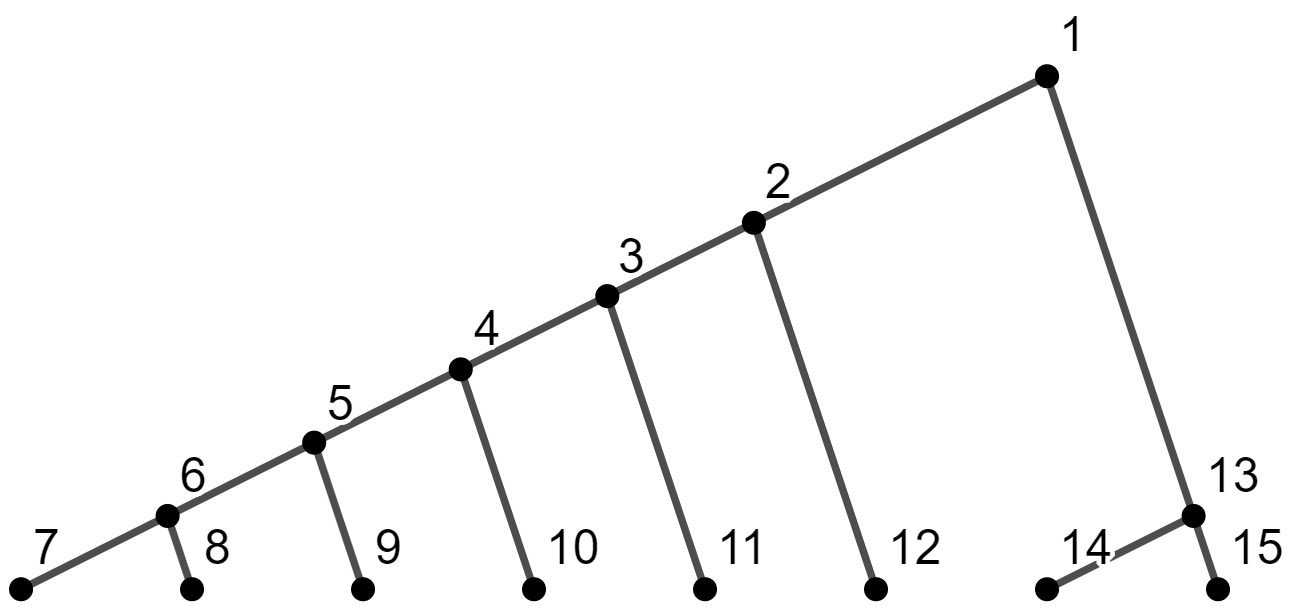
\includegraphics[width=0.6\textwidth]{figures/rooted_tree.jpg}
    \captionsetup{singlelinecheck=off}
    \caption{The illustration suggests, that the node $1$ is the root of the tree. Together with some function $l:\;\{1,..15\} \mapsto \{A,B,C\}$ $T$ is a rooted labelled tree.} \end{figure}
\begin{defin}
Let $T=(V,E)$ be a rooted labelled tree with root $r\in V$. We define the \textit{parent} $P(v) \in V$ of a node $v\in V\setminus \{r\}$ to be direct predecessor of $v$ on the unique path from $r$ to $v$ in $T$. The parent of $r$ is undefined. 
\end{defin}
\begin{defin}
Let $T=(V,E)$ be a rooted labelled tree with root $r\in V$, let $w,v \in V$. The node $w$ is a \textit{child} of $v$ if and only if $v$ is the parent of $w$. We denote by $C_T(v)$ the \textit{set of all children} of $v$:
$$ C_T(v):= \{w \in V | P(w) = v\}.$$
If the setting is clear one can use the shortcut $C(v)$ for $C_T(v)$
\end{defin}
\begin{defin}
Let $T=(V,E)$ be a rooted labelled tree with root $r\in V$, let $w \neq v \in V\setminus \{r\}$. The node $w$ is a sibling of $v$ if and only if $P(v) = P(w)$. We denote by $S(v)$ the \textit{sibling group of v}:
$$ S(v) := \{w \in V | P(w) = P(v)\}.$$
For the special case of the root $r$ we define the sibling group manually by $S(r) := \{r\}$.
\end{defin}
\begin{rem}
Note that for a node $v$ the following inclusion holds naturally:
$$v \in S(v)$$
That also implies that $|S(v)| >=1$.
\end{rem}
\begin{defin}
Let $T=(V,E)$ be a rooted tree. We call $T$ \textit{ordered} if all siblings have a specific and fixed order among each other. 
\end{defin}
\begin{figure}[h!]
	\begin{center} 
		\begin{tabular}{c}
		\xymatrix @R=4mm @C=2mm{
			&T_1&&&&&&T_2&\\
			&*+[o][F-]{A}\ar@{-}[dl]\ar@{-}[dr]&&&&&&*+[o][F-]{A}\ar@{-}[dl]\ar@{-}[dr]&\\
			*+[o][F-]{B}&&*+[o][F-]{C}&&&&*+[o][F-]{C}&&*+[o][F-]{B}
			}
		\end{tabular}
		\caption{If we assume that $T_1$ and $T_2$ are unordered trees, then $T_1 = T_2$. But if we consider them to be ordered from left to right as in the figure, then $T_1 \neq T_2$.}
	\end{center}
\end{figure}
\begin{defin}
Let $T=(V,E)$ be a rooted ordered tree with root $r\in V$ and let $n:= |V|$. The \textit{post-order index} is a way of enumerating the nodes of $T$ from $1$ to $n$. For that, you perform the following routine recursively starting with $v=r$ and index $m=1$:\\
\end{defin}\newpage
\begin{algorithm} % enter the algorithm environment
\caption{Assign the \textit{post-order} index to a tree $T$} % give the algorithm a caption
\label{alg1} % and a label for \ref{} commands later in the document
\begin{algorithmic}
\Function{Routine}{$v$, $m$}  
\If {($v$ is a leave) or (all children of $v$ are indexed)}
	\State Index $v$ with the index $m$;
	\State \Call{Routine}{$P(v)$, $m+1$}
\Else 
	\State Let $w$ be the left-most child of $v$ that has not yet been indexed.
	\State \Call{Routine}{$w$,$m$};
\EndIf
\EndFunction
\end{algorithmic}
\end{algorithm}
\begin{figure}[!ht]
	\begin{displaymath}
	\xymatrix @R=3mm @C=3mm{
		&&&T&&&\\
		&&&*+[o][F-]{13}\ar@{-}[d] &&&\\
		&&&*+[o][F-]{12}\ar@{-}[d] \ar@{-}[dll] \ar@{-}[drr]&&\\
		&*+[o][F-]{5} \ar@{-}[d]&&*+[o][F-]{6}&&*+[o][F-]{11} \ar@{-}[d]\\
		&*+[o][F-]{4} \ar@{-}[dl] \ar@{-}[d] \ar@{-}[dr]&&&&*+[o][F-]{10} \ar@{-}[dl] \ar@{-}[d] \ar@{-}[dr]\\
		*+[o][F-]{1}&*+[o][F-]{2}&*+[o][F-]{3}&&*+[o][F-]{7}&*+[o][F-]{8}&*+[o][F-]{9}	
	}
	\end{displaymath}
	\caption{An example of the post order indexing. Note that for every subtree the root is indexed at last.}
	\label{fig:postorder}
\end{figure} 
\begin{defin} Let $T=(V,E)$ be an ordered tree rooted at $r \in V$. If $|V| > 1$ we denote by $T^{\circ} := T \setminus \{r\}$ be the forest, which results from $T$ after deleting the root $r$. Moreover for a node $v\in V$ we denote by $F_v$ the subtree of $T$ rooted at $v$. 
\end{defin}
\begin{defin} Let $T=(V,E)$ be an ordered forest. We denote by $L_T$ and $R_T$ the left- and rightmost subtrees of $T$ respectively. Furthermore the roots of $L_T$ and $R_T$ are denoted by $l_T$ and $r_T$ respectively
\end{defin}
\begin{rem}
Consider the tree $T$ in Figure~\ref{fig:postorder}. Then we can use the notion introduced above to describe the following trees:
\begin{figure}[!ht]
	\begin{subfigure}[b]{0.49\textwidth}
	\caption{$T^{\circ}$}
	\begin{displaymath}
	\xymatrix @R=3mm @C=3mm{
		&&&*+[o][F-]{12}\ar@{-}[d] \ar@{-}[dll] \ar@{-}[drr]&&\\
		&*+[o][F-]{5} \ar@{-}[d]&&*+[o][F-]{6}&&*+[o][F-]{11} \ar@{-}[d]\\
		&*+[o][F-]{4} \ar@{-}[dl] \ar@{-}[d] \ar@{-}[dr]&&&&*+[o][F-]{10} \ar@{-}[dl] \ar@{-}[d] \ar@{-}[dr]\\
		*+[o][F-]{1}&*+[o][F-]{2}&*+[o][F-]{3}&&*+[o][F-]{7}&*+[o][F-]{8}&*+[o][F-]{9}	
	}
	\end{displaymath}
	\end{subfigure}
	\begin{subfigure}[b]{0.49\textwidth}
	\caption{$T_{12}^{\circ}$}
	\begin{displaymath}
	\xymatrix @R=3mm @C=3mm{
		&*+[o][F-]{5} \ar@{-}[d]&&*+[o][F-]{6}&&*+[o][F-]{11} \ar@{-}[d]\\
		&*+[o][F-]{4} \ar@{-}[dl] \ar@{-}[d] \ar@{-}[dr]&&&&*+[o][F-]{10} \ar@{-}[dl] \ar@{-}[d] \ar@{-}[dr]\\
		*+[o][F-]{1}&*+[o][F-]{2}&*+[o][F-]{3}&&*+[o][F-]{7}&*+[o][F-]{8}&*+[o][F-]{9}	
	}
	\end{displaymath}
	\end{subfigure}
	\begin{subfigure}[b]{0.32\textwidth}
	\caption{$L_{T_{12}^{\circ}} = T_5$}
	\begin{displaymath}
	\xymatrix @R=3mm @C=3mm{
		&*+[o][F-]{5} \ar@{-}[d]&\\
		&*+[o][F-]{4} \ar@{-}[dl] \ar@{-}[d] \ar@{-}[dr]&\\
		*+[o][F-]{1}&*+[o][F-]{2}&*+[o][F-]{3}&
	}
	\end{displaymath}
	\end{subfigure}
	\begin{subfigure}[b]{0.32\textwidth}
	\caption{$R_{T_{12}^{\circ}} = T_{11}$}
	\begin{displaymath}
	\xymatrix @R=3mm @C=3mm{
		&*+[o][F-]{11} \ar@{-}[d]\\
		&*+[o][F-]{10} \ar@{-}[dl] \ar@{-}[d] \ar@{-}[dr]\\
		*+[o][F-]{7}&*+[o][F-]{8}&*+[o][F-]{9}	
	}
	\end{displaymath}
	\end{subfigure}
	\begin{subfigure}[b]{0.32\textwidth}
	\caption{$R_{T_{12}^{\circ}}^{\circ} = T_{11}^{\circ} = T_{10}$}
	\begin{displaymath}
	\xymatrix @R=3mm @C=3mm{
		&*+[o][F-]{10} \ar@{-}[dl] \ar@{-}[d] \ar@{-}[dr]\\
		*+[o][F-]{7}&*+[o][F-]{8}&*+[o][F-]{9}	
	}
	\end{displaymath}
	\end{subfigure}
	\caption{Different subtrees using the introduced notion.}
	\label{fig:subtrees}
\end{figure} 
\end{rem}
\begin{defin} Let $T_i=(V_i,E_i)$ be an rooted tree. We denote by $t_i:= |V_i|$ the size of the input graph. Furthermore we use the notion of $t_{l,i}$ for the number of leaves in $T_i$ and $t_{h,i}$ for the length of the longest path from the root to any leaf. 
\end{defin}
\begin{rem}
We will need this definitions mainly for stating the running times of algorithms. Since we want to compare $T_1$ with $T_2$ we need to be able to separate those numbers accordingly. Furthermore we will always assume w.l.o.g. $O(t_1)\geq O(t_2)$.
\end{rem}
\begin{defin}
Let $T$ be a forest which is ordered according to the post order indexing. Let $T'$, $T''$ be two induced subforests of $T$ with $\exists i_{T'},j_{T'},i_{T''},j_{T''}$ s.t. $V(T')=\{i_{T'},...,j_{T'}\}$ and $V(T'')=\{i_{T''},...,j_{T''}\}$.\\
We call $T'$ to a \textit{prefix} of $T''$ if and only if the following holds:
$$i_{T'} = i_{T''} \quad \text{and} \quad j_{T'} \leq j_{T''}$$
\end{defin}
\begin{defin}
Let $T$ be an ordered tree rooted at $r$. Then we define the \textit{keyroots} of $T$ to be set of all nodes that have a left sibling:
$$\text{keyroots}(T) := \{r\} \cup \{v \in V(T) \,|\,v\text{ has a left sibling}\}.$$\\
Assume $T$ is an ordered forest with trees $T_1,...,T_n$ rooted at $r_1,...r_n$. Then we define the set of keyroots as the union of the separated sets of keyroots:
$$\text{keyroots}(T) = \sideset{}{}\bigcup_{i=1}^n \text{keyroots}(T_i).$$
\end{defin}
\begin{defin}
Let $T$ be an ordered tree rooted at $r$. For a node $v$ we define the \textit{collapse depth} of $v$ cdepth$(v)$ to be the number of keyroot ancestors of $V$:
$$\text{cdepth}(v) = |\{w \in V(T)\,|\, w \text{ is an ancestor of }v\} \cap \text{keyroots}(T)|.$$
\end{defin}
\begin{defin}
Let $T$ be an ordered tree rooted at $r$. For every non-leaf node $n$ we choose one node $m \in C(n)$ among those with the most descendants in $C(n)$ arbitrarily. We define $m$ to be a heavy node. All non-heavy nodes are defined as \textit{light}, especially the root $r$. 
\end{defin}
\begin{rem}
In most cases a tree has multiple possibilities for the definition of heavy nodes. For example if there are multiple leaves with the same parent.
\end{rem}
\begin{defin}
Let $T$ be an ordered tree rooted at $r$ and let there be a fixed definition of heavy nodes. We call an edge to be \textit{heavy} if it connects a non-leaf with its heavy child. Furthermore we call a path, which connects a light node with a leaf and only consists of heavy edges a heavy path. We call the heavy path originating at the root $r$ the \textit{main heavy path}. The set of all heavy paths is called a \textit{heavy path decomposition}. 
\end{defin}
\begin{rem}
Light leaves are a special case of heavy paths of length 0.
\end{rem}
\begin{rem}
The heavy path decomposition depends on the choice of heavy nodes.
\end{rem}
\begin{figure}[!ht]
	\centering
	\begin{subfigure}[b]{0.45\textwidth}
	\caption{}
	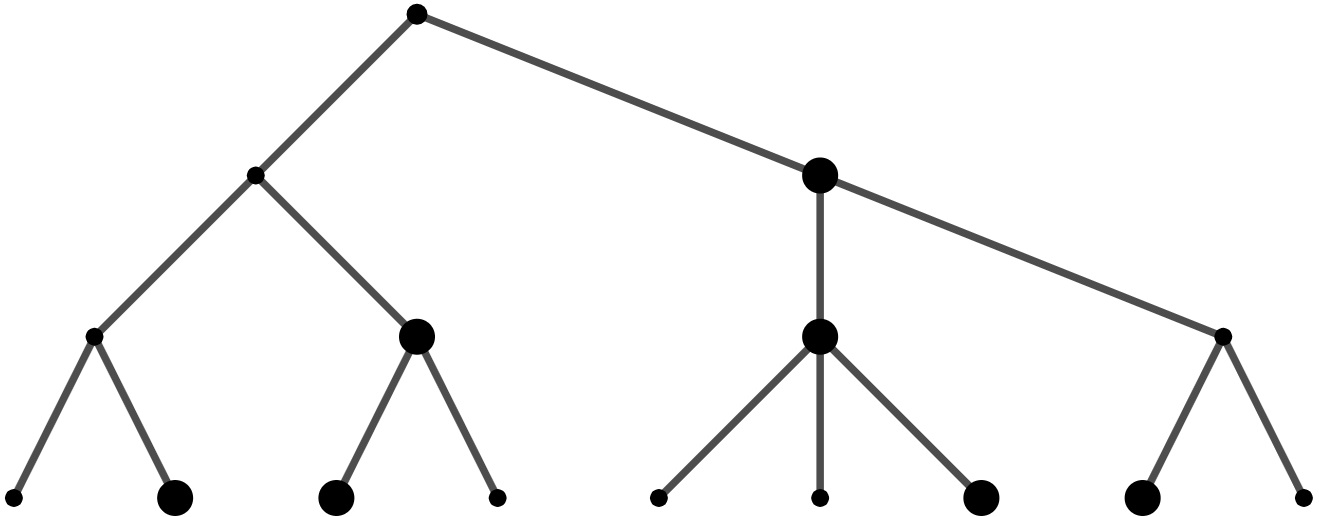
\includegraphics[width=\textwidth]{figures/heavy_nodes.jpg}
    \end{subfigure}
    \begin{subfigure}[b]{0.45\textwidth}
	\caption{}
	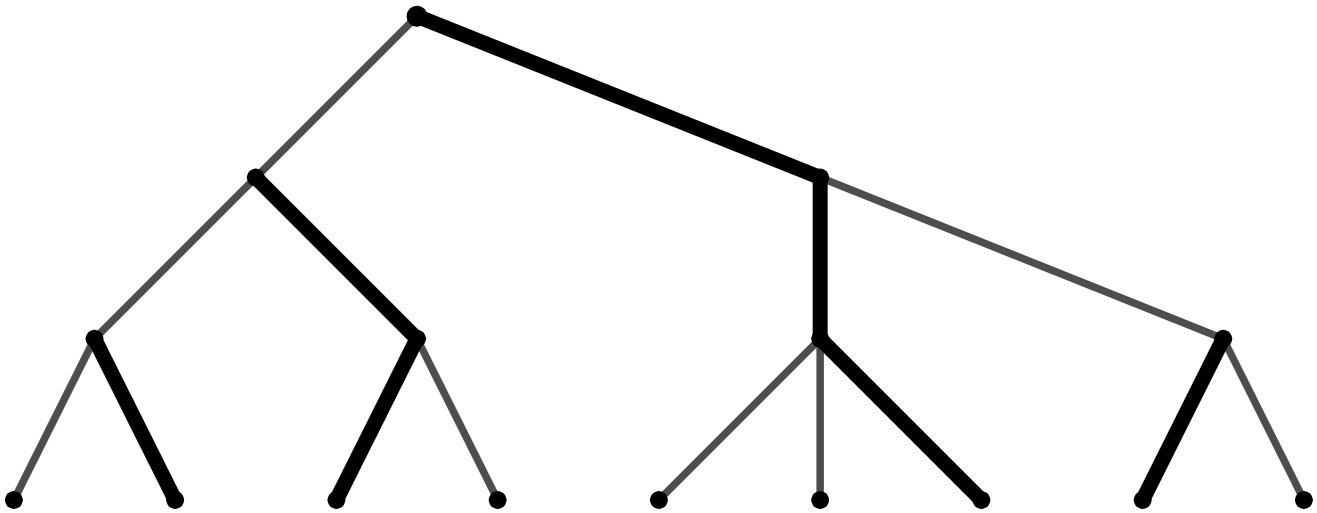
\includegraphics[width=\textwidth]{figures/heavy_path_decomposition.jpg}
    \end{subfigure}
	\caption{Example of a heavy path decomposition. Figure a) shows the heavy nodes, Figure b) the correspondig heavy paths.}\label{fig:heavypath}
\end{figure}
\begin{defin}
Let $T$ be an ordered tree rooted at $r$, $v \in V(T)$ and suppose a heavy path decomposition is fixed. we define the \textit{light depth} ldepth$(v)$ to be the number of light proper ancestors of $v$.\\
Furthermore we define ldepth$(T)$ as follows:
$$\text{ldepth}(T) = \max \{\text{ldepth}(v) \,|\,v \in T\}.$$
\end{defin}
\begin{defin}
Let $T$ be an ordered tree rooted at $r$ and let a heavy path decomposition be given. We define the set TopLight$(T)$ to be the set of all light nodes $v \in V$ with ldepth$(v) = 1$:
$$\text{TopLight}(T) := \{v \,|\,\text{ldepth}(v)=1 \text{ and } v \text{not in the main heavy path of }T\}.$$
\end{defin}
\begin{rem}
A light node $v\in V(T)$ is in TopLight$(T)$ if and only if its parent lies on the main heavy path of $T$.
\end{rem}
\begin{defin} Let $T$ be a tree, $X$ the set of leaves of $T$ and $\Sigma$ a set of labels. Then $T$ is an \textit{unrooted phylogenetic} tree if all leaves are labelled bijectively with some label in $\Sigma$, all interior leaves are unlabelled and all interior nodes have degree at least three. A \textit{rooted phylogenetic} tree is a phylogenetic tree where one node, the root $r \in V(T)$, is distinguished from the others and may have degree two.  
\end{defin}
\begin{defin} Let $T$ be a phylogenetic tree, $X$ the set of leaves of $T$ and $\Sigma$ the set of labels of $X$. Then $\Sigma$ is called the set of \textit{taxa}. 
\end{defin}
\begin{defin} Let $T$ be a phylogenetic tree and $X$ the set of leaves of $T$. Some $C \subset X$ is called a \textit{clade} if $\exists \,v \in T$ s.t. $C$ is the set of leaves in the induced subtree $T_v$ of $T$. A clade $C$ is called \textit{trivial} if $|C|=1$ or $C = X$. The set $\mathcal{C}(T) := \{C \subset V\;|\; C\text{ is a clade}\}$ is the set of clades of $T$, $\mathcal{C}^*(T) := \{C \in \mathcal{C}(T)\;|\; C\text{ is non trivial}\}$ the set of non trivial clades.
\end{defin}
\begin{defin} Let $T$ be a binary tree. $T$ is called \textit{full}, if every inner node has exactly two children.
\end{defin}


\section{Other necessary Tools}
\begin{defin}
Let $T=(V,E)$ be a rooted labelled tree. The so called \textit{basic tree edit operations} on $T$ are \textit{relabelling, inserting} and \textit{deleting}: 
\begin{enumerate}
\item \textit{Relabelling $v$:} changing the label of a node $v$.
\item \textit{Inserting $v$ underneath $v'$: } insert a new node $v$ into $T$ as a child of $v'$ and assign the children of $v'$ to the new node $v$. Denote the new tree by $T'$, then: 
$$C_{T'}(v') = \{v\}\text{ and }C_{T'}(v) = C_T(v')$$.
\item \textit{Deleting $v$ underneath $v'$: } the opposite transformation of inserting. Delete $v$, assign all children of $v$ to $v'$ in the same order. Denote the new tree by $T'$, then: 
$$C_{T'}(v') = C_T(v')\setminus \{v\} \cup C_T(v)$$.
\end{enumerate}
\end{defin}
\begin{figure}[b]
	\captionsetup[subfigure]{labelformat=empty}
	\centering
	\begin{subfigure}[b]{0.18\textwidth}
	\caption{}
	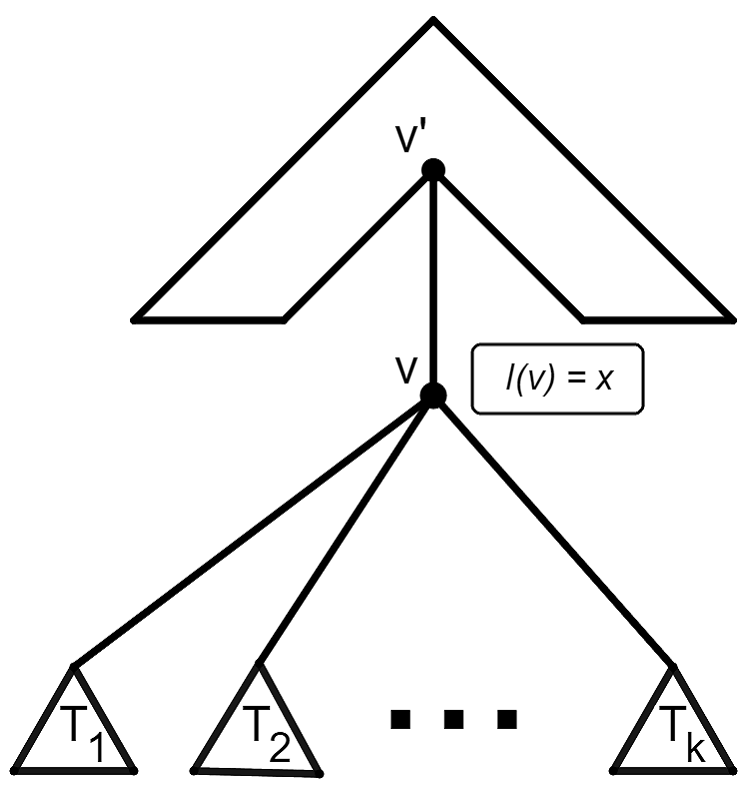
\includegraphics[width=\textwidth]{figures/TreeEditOperation_1.png}
    \end{subfigure}
    \begin{subfigure}[b]{0.18\textwidth}
	\caption{}
	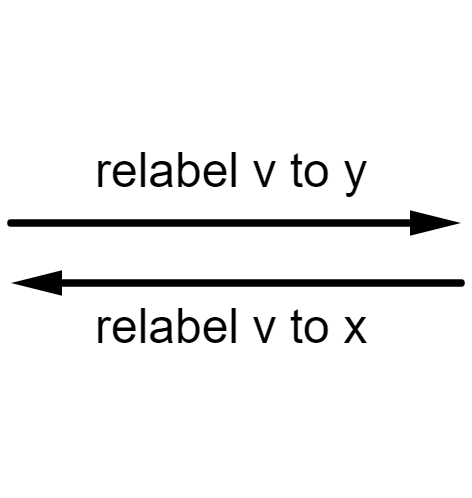
\includegraphics[width=\textwidth]{figures/TreeEditOperation_1,5.png}
    \end{subfigure}
    \begin{subfigure}[b]{0.18\textwidth}
	\caption{}
	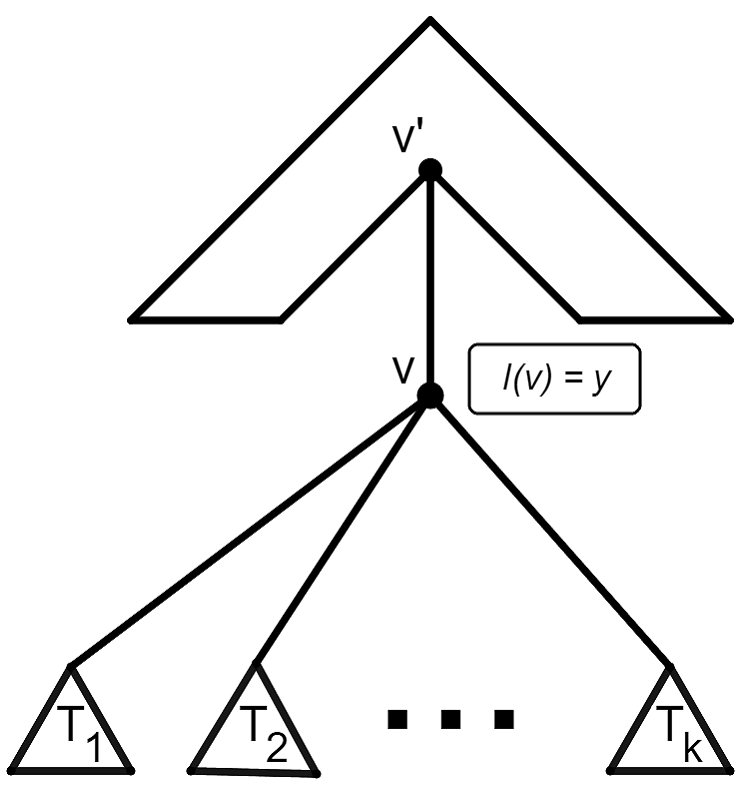
\includegraphics[width=\textwidth]{figures/TreeEditOperation_2.png}
    \end{subfigure}
    \begin{subfigure}[b]{0.18\textwidth}
	\caption{}
	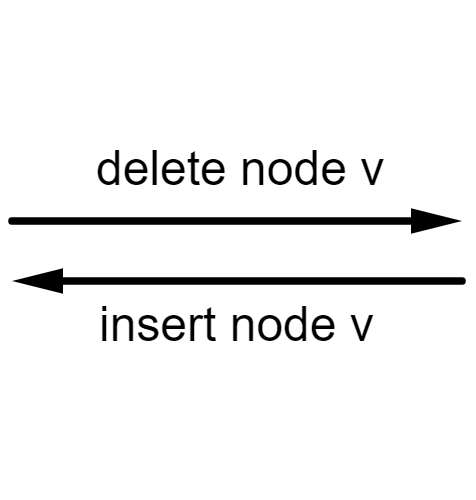
\includegraphics[width=\textwidth]{figures/TreeEditOperation_2,5.png}
    \end{subfigure}
    \begin{subfigure}[b]{0.18\textwidth}
	\caption{}
	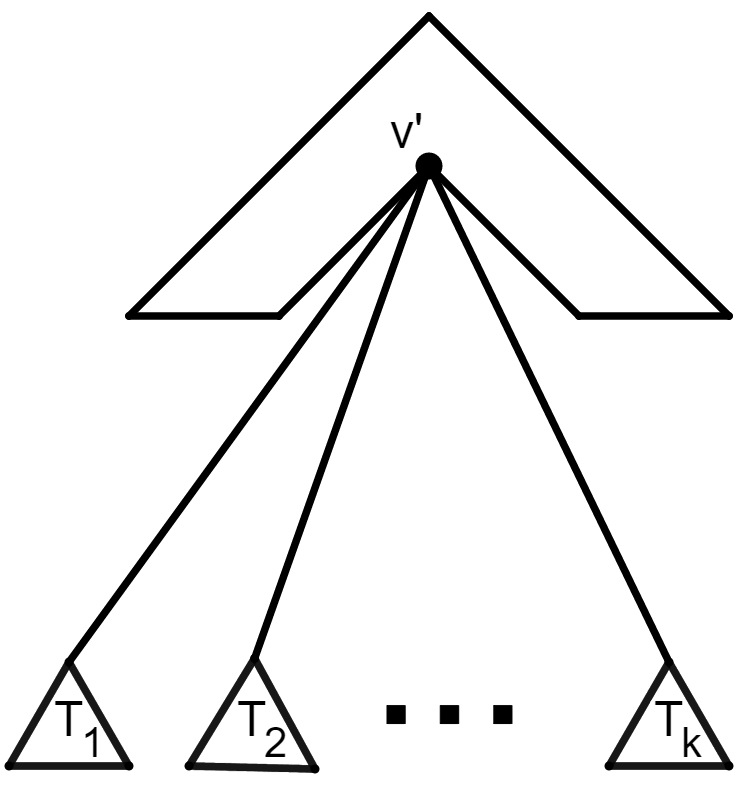
\includegraphics[width=\textwidth]{figures/TreeEditOperation_3.png}
    \end{subfigure}
	\caption{Illustration of the basic tree edit operations relabelling, deleting and inserting.}\label{fig:heavypath}
\end{figure}
\begin{defin}
Let $T=(V,E)$ be a rooted labelled tree and let $o$ be one of the basic edit operations defined above. We denote by $o(T)$ the tree that we get after executing the operation $o$ on the tree $T$. \\
Furthermore let $o'=(o'_1,o'_2,...,o'_n)$ be a finite sequence of basic edit operations. We define $o'(T)$ as the consecutive application of the basic operations:
$$o'(T) := o'_n(o'_{n-1}(...(o'_1(T)...)).$$
\end{defin}
\begin{defin}
Let $T=(V,E)$ be a rooted labelled tree, let $\Sigma$ be the set of labels and $\sigma, \sigma' \in \Sigma$. Furthermore let $o$ be one of the basic edit operations defined above. Then the cost of $c(o)$ is defined as:
\[
c(o) :=
\begin{dcases*}
        c_{rel}(\sigma, \sigma')  & Relabelling existing node $v$ from $\sigma$ to $\sigma'$\\
        c_{ins}(\sigma) & Inserting new node $v$ with label $\sigma$ \\
        c_{del}(\sigma) & Deleting existing node $v$ with label $\sigma$
\end{dcases*} 
\]
Moreover let $o'=(o'_1,...o'_n)$ be a finite sequence of basic edit operations. We define the costs of $o'$ to be the sum of costs of the individual operations:
$$c(o') := \sideset{}{}\sum_{i=1}^n c(o'_i).$$
\end{defin}
\begin{rem}
Because of the symmetry we can assume $c_{del}(\sigma) = c_{ins}(\sigma)$. Because of that, we will only work with relabelling and deleting operations later on.
\end{rem}
\begin{defin}
Let $T=(V,E)$ be a rooted labelled tree and let $o$ be one of the basic edit operations defined above. Then the cost of $c(o)$
\end{defin}
\begin{defin}
Let $T=(V,E)$ be a rooted labelled tree. A function $d: V\times V \mapsto \mathcal{R}$ is a \textit{metric} if the following conditions are fulfilled $\forall u,v,w, \in V$:
\begin{enumerate}
\item $d(v,w) \geq 0$
\item $d(v,w) = 0 \iff v=w$
\item $d(v,w) = d(w,v)$
\item $d(u,w) \leq d(u,v) + d(v,w)$
\end{enumerate}
\end{defin}

\begin{defin}
The \textit{Catalan numbers} $(C_n)_{n \in \mathbb{Z}_{\geq 0}}$ forms a sequence of natural numbers which occur in many recursively defined combinatorial problems. They are recursively defined as follows:
\begin{align*}
C_0 &= 1
C_n &= \sum_i^{n-1} \; C_i C_{n-i-1} \text{ for } n \geq 1 
\end{align*}
\end{defin}
\begin{rem}
The following two combinatorial problems are examples in which the Catalan numbers occur:
\begin{itemize}
\item Counting the number of expressions containing $n$ pairs of parentheses where any prefix of the expression contains at least as many opening parentheses "(" as closing ones ")".
\item Counting the number of full binary trees with $n+1$ leaves.
\end{itemize}
\end{rem}

\chapter{Tree Edit Distance}
In this chapter we will discuss the so called \textit{tree edit distance}. This chapter is based on Demaine et al.'s paper about an optimal decomposition algorithm []. 

\section{Introduction} 
\begin{defin} \label{def:ted}
Let $T_1=(V_1,E_1)$ and $T_2=(V_2,E_2)$ be two rooted ordered labelled trees together with a set of labels $\Sigma$. Furthermore let the costs for the basic edit operations relabelling, inserting and deleting be fixed. \\
Let $o^*:= (o^*_1,...,o^*_n)$ be a finite sequence of edit operations that fulfills the following:
\begin{align*}
o^*(T_1) &= o^*_n(...(o^*_1(T_1)) = T_2 \\
c(o^*) = \sideset{}{}\sum_{i=1}^n c(o^*_i) &= \sideset{}{}\min_{\substack{o\text{ sequence of}\\ \text{edit operations}}} \{c(o)\,|\,o(T_1)=T_2\}
\end{align*}
Then the \textit{tree edit distance} $\delta(T_1,T_2)$ is defined as:
$$\delta(T_1,T_2) := c(o^*).$$
\end{defin}
\begin{defin}
Let $T_1=(V_1,E_1)$ and $T_2=(V_2,E_2)$ be two rooted ordered labelled forests and the rest as in the definition~\ref{def:ted}. Then we can extend the definition of the tree edit distance $\delta(T_1,T_2)$ trivially. 
\end{defin}

The origin of finding the tree edit distance is an intuitive way of comparing two trees. Given two labelled ordered trees $T_1$ and $T_2$. What is the cheapest sequence of edit operations that transforms $T_1$ into $T_2$? Take a look at the trees $T_1$ and $T_2$ in~\ref{fig:TEE} and the sequence of operations that performs the transformation from $T_1$ to $T_2$. If we assume, for example, that every operation costs the same then the sequence shown in the figure would be an optimal one.
\begin{figure}[!h]
    \centering
    \begin{subfigure}[b]{\textwidth}
		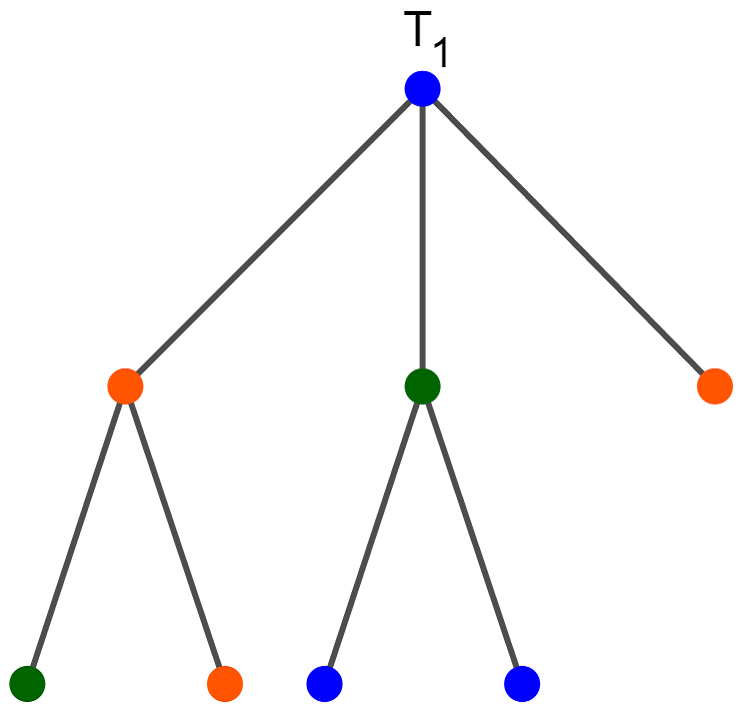
\includegraphics[width=0.39\textwidth]{figures/TreeEditExample_1.jpg}
		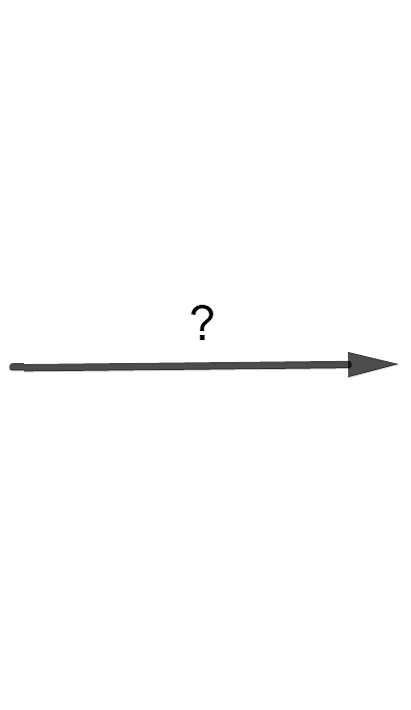
\includegraphics[width=0.2\textwidth]{figures/TreeEditExample_1,5.jpg}
		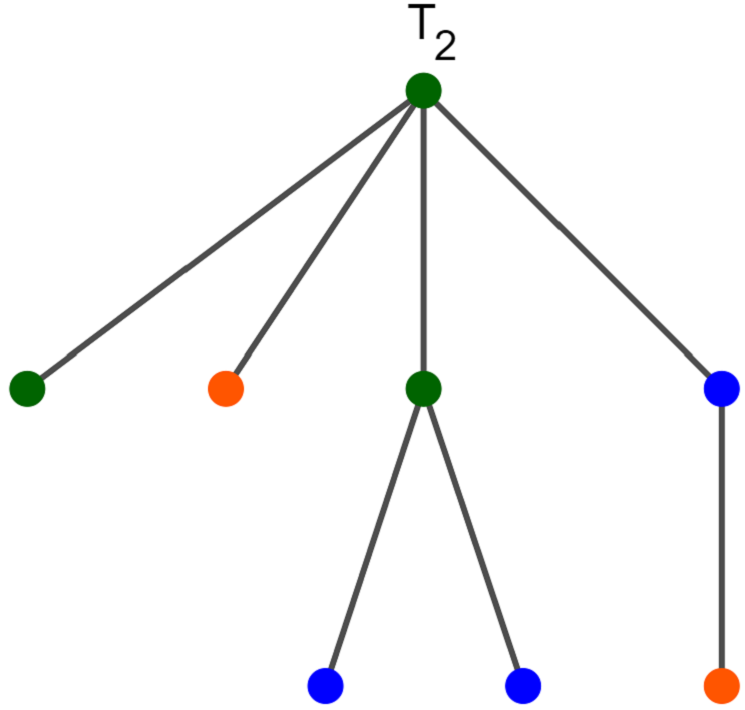
\includegraphics[width=0.39\textwidth]{figures/TreeEditExample_2.jpg}
		\caption{Consider these two trees $T_1$ and $T_2$. Finding the cheapest way of transforming $T_1$ into $T_2$ can be really hard. Underneath we see one sequence of editing operations that could be the cheapest one.}
	\end{subfigure}
    \begin{subfigure}[b]{\textwidth}
		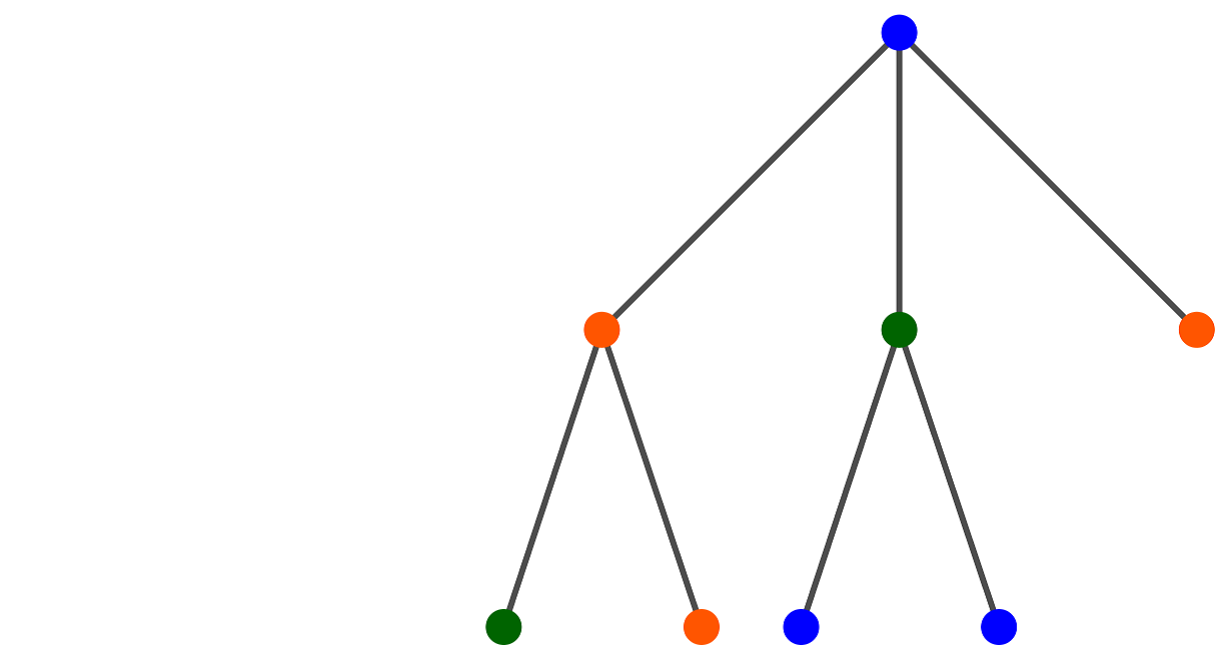
\includegraphics[width=0.45\textwidth]{figures/TreeEditExample_3.jpg}
		\quad
		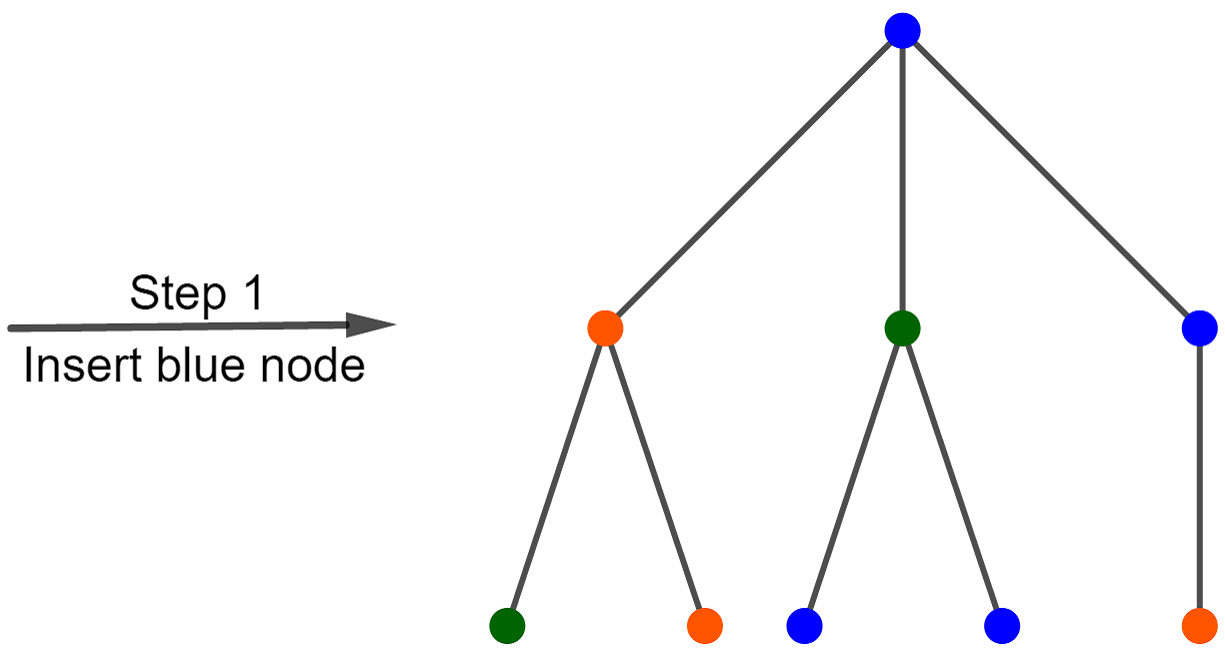
\includegraphics[width=0.45\textwidth]{figures/TreeEditExample_4.jpg}
		\\ %comment
		\\
		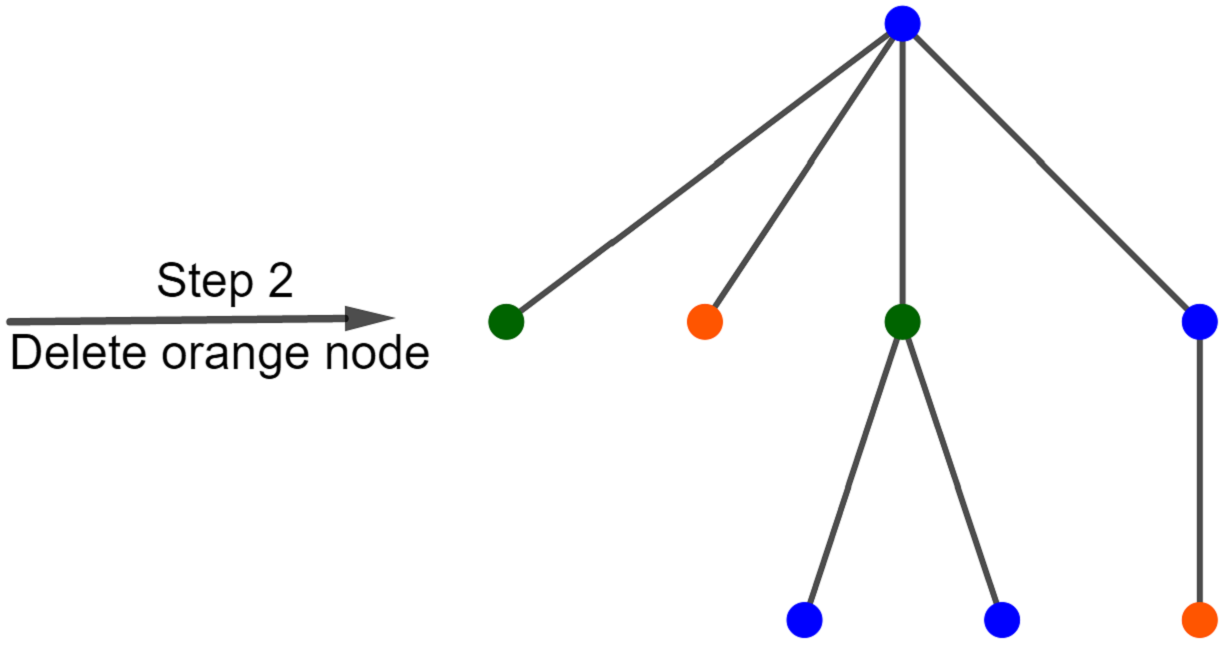
\includegraphics[width=0.45\textwidth]{figures/TreeEditExample_5.jpg}
		\quad
		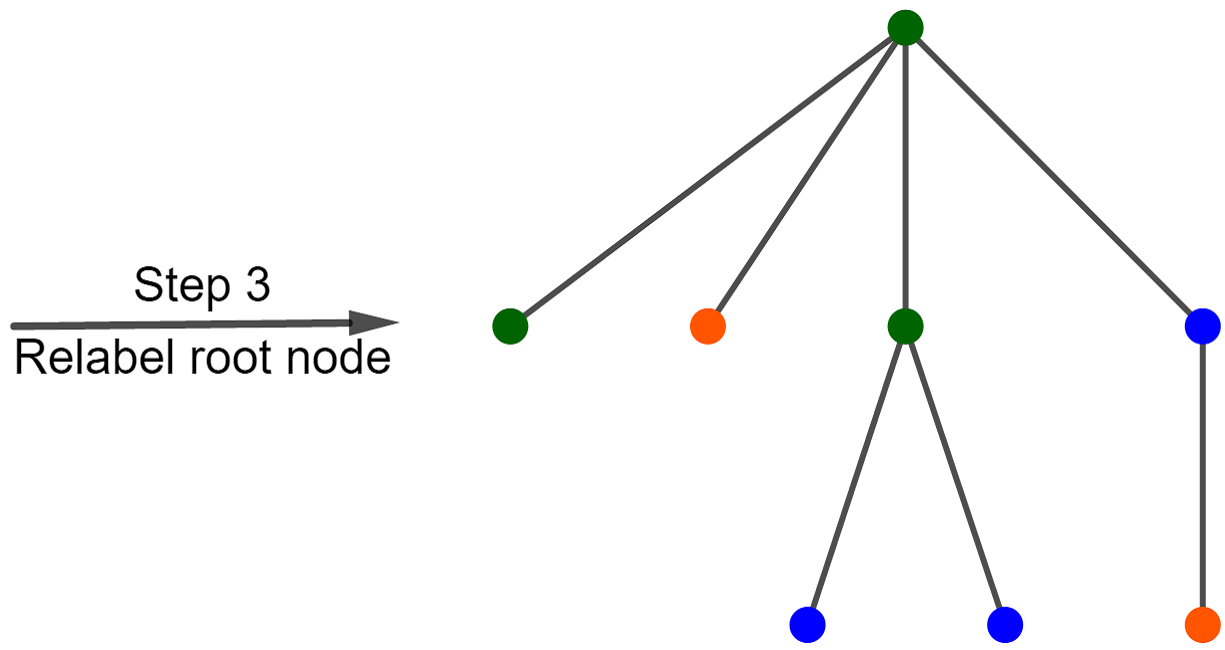
\includegraphics[width=0.45\textwidth]{figures/TreeEditExample_6.jpg}
		\caption{Step 1: Insert a node right above the rightmost child of the root. Step 2: Delete the leftmost child of the root. Step 3: Relabel the root node.}
	\end{subfigure}
	\label{fig:TEE}
\end{figure}
The tree edit distance is used in the fields of structured text databases, computer vision and in bioinformatics. In the last field one needs to compare the secondary structure of RNA-molecules without the disadvantages of other approaches. For a more detailed description about this topic please take a look at [].

\section{Short History of the Tree Edit Distance}
The tree edit distance was introduced by Tai in the year 1979~\cite{Tai}. In addition to the definition he also provided an algorithm to compute the tree edit distance. The running time and space complexity amounts to $O(t_{l,1}^2 t_{l,2}^2 t_1 t_2)$ which implies a worst-case running time of $O(t_1^6)$. \\
It took about a century until Shasha and Zhang~\cite{SasAndZha} came up with a dynamic programming approach that improved the running time to $O(t_1^2 t_2^2)$. Later on Klein~\cite{Kle} started with his algorithm, changed the way to of branching and was able to further improve the running time to $O(t_1 t_2^2 \log t_1)$ time. Dulucq and Touzet~\cite{DulAndTou} proved a lower bound of $\Omega(t_1 t_2 \log t_1 \log t_2)$ on the running time for all algorithms for the tree edit distance which are based on dynamic programming in 2003. Finally, in 2007 Demaine et al.~\cite{Dem} provided an algorithm that satisfies the lower bound on dynamic programming approaches.\\
Chen~\cite{Che} presented a different approach relying on fast matrix multiplication solving the tree edit distance problem in $O(t_1 t_2 + t_1 t_{2,l}^2 + t_{1,l}t_{2,l}^{2.5})$ time and $O(t_1 + (t_2 + t_{2,l}^2)\min \{t_{1,l},t_{2,l}\})$ space. You can also take a look at other algorithms, see~\cite{Apo, Bil, Val}

In this thesis we will concentrate on the dynamic programming approaches of Shasha and Zhang, Klein and last but not least Demaine et al. But since this thesis tries to show different comparing mechanisms we will keep it rather short. If you want to have a more detailed description about something, please take a look into the original papers.

\section{Dynamic Programming Approach}
The key for any dynamic programming approach is to find a suitable way for branching a hard problem into smaller and therefore easier subproblems. 
\begin{defin}
Let $T_1,T_2$ be two rooted labelled ordered forests and let the cost functions be defined as stated in the definition.
Consider the problem of computing $\delta(T_1,T_2)$ with a fixed dynamic programming approach $A$. A \textit{relevant subproblem} of $(T_1,T_2)$ is any pair of rooted labelled forests $(T_1',T_2')$ such that the following holds:\\
During the computation of $\delta(T_1,T_2)$ we encounter the problem of solving $\delta(T_1',T_2')$. We define $\mathcal{R}_A$ to be the set of all relevant subproblems\\
We call $(T_1',T_2')$ to be a trivial subproblem if and only if $(T_1',T_2')$ is a relevant subproblem and $\exists i \in \{1,2\}$ s.t. $T_i' = (\emptyset,\emptyset)$. We defnine $\mathcal{T}_A \subset \mathcal{R}_A$ to be set of all trivial subproblems.
\end{defin}
\begin{rem}
Since a relevant subproblem $(T_1',T_2')$ occurs in the computation of $\delta(T_1,T_2)$, there has to exist a sequence of basic editing operations $o$ only consisting of relabelling and deleting operations s.t. $o(T_1)=T_i' \, \forall i \in \{1,2\}$.
\end{rem}
\begin{rem}
We only consider deleting and relabelling operations because of the symmetry between deleting a node in $T_1$ and inserting a proper node in $T_2$ vice versa.
\end{rem}
\begin{rem}
A trivial dynamic programming approach would lead to $\Omega(2^{t_1+t_2})$ subproblems. Therefore it is necessary to branch in a smart way to get a polynomial number of relevant subproblems.
\end{rem}
The idea of branching is to consider the two rightmost or leftmost roots of $T_1$ and $T_2$. Either one of those two gets deleted or the two roots are matched. In the first case you result in a new smaller relevant subproblem, in the latter you even end up with two separated relevant subproblems:\\
Suppose you match $r_{T_1}$ with  $r_{T_2}$. Then any node from $R_{T_1}$ that gets matched with a node in $T_2$ has to be matched with a node in $R_{T_2}$ because of the strict ancestry relation. So matching those two roots splits the problem of computing $\delta(T_1,T_2)$ into the two subproblems of computing $\delta(R_{T_1}^{\circ},R_{T_2}^{\circ})$ and $\delta(T_1-R_{T_1},T_2-R_{T_2})$.
\begin{defin}
Consider the problem of computing the tree edit distance $\delta(T_1,T_2)$ with a dynamic programming approach $A$.\\
We call $S_A : \mathcal{R}_A \mapsto \{\text{left,right}\}$ the \textit{decomposition strategy} of the dynamic programming approach $A$ if for any relevant subproblem  $(T_1',T_2') \in \mathcal{R}_A$ the following holds: \\
The direction $S_A((T_1',T_2'))$ coincides with the direction of branching according to the dynamic programming approach $A$.
\end{defin}


\subsection{Shasha and Zhang's algorithm}
Shasha and Zhangs algorithm is the most basic dynamic programming approach. They restrict themselves to the decomposition strategy that always chooses the right direction. 
\begin{lem}\label{lem:sets}
Let $T_1,T_2$ be two rooted labelled forests and assume these forests are ordered according to the post order indexing. Consider the problem of computing  $\delta(T_1,T_2)$ with a dynamic programming approach $A$ that has a decomposition strategy $S_A(T_1',T_2') = \text{right} \, \forall (T_1',T_2') \in \mathcal{R}_A \setminus \mathcal{T}_A$. Then:\\
$\forall (T_1',T_2') \in \mathcal{R}_A \setminus \mathcal{T}_A : \exists \, i_1 \leq j_1,\, i_2 \leq j_2 \in \mathcal{N}$ s.t.:\\
 \begin{align*}
 V(T_1') &= \{i_1,i_1+1,...,j_2\} \\
 V(T_2') &= \{i_2,i_2+1,...,j_2\}.
 \end{align*}
\end{lem}
\begin{rem}[Remark 1]
Because of the post order indexing, the rightmost root $r_T$ has the highest overall index.
\end{rem}
\begin{rem}[Remark 2] 
For two induced subtrees $T_{v'}$ and $T_{v''}$ of $T$ s.t. $V(T') \cup V(T'') = \emptyset$ assume that $v'$ lies on the left of $v''$. Then the index of every node in $T_{v'}$ is strictly smaller than the index of all nodes in $T_{v''}$.
\end{rem}
\begin{proof}
We make an inductive argument. We start with our base: For $T_1$ and $T_2$ the claim is trivially true. So let's consider an induction step and assume that the claim holds for a relevant subproblem $(T_1',T_2')$. Therefore there exists the indexes $i_1,j_1,i_2,j_2$ as in the lemma. We have three possible induction steps:
\begin{enumerate}
\item \textit{Delete $r_{T_1'}$:} If $i_1 \leq j_1-1$ the new indexes will be $i_1,j_1-1,i_2,j_2$ because of Remark 1. Otherwise we just deleted the only node left in $T_1' \Rightarrow $ the new relevant subproblem $(T_1'',T_2'') \in \mathcal{T}_A$
\item \textit{Delete $r_{T_2'}$:} Equivalent to the previous case.
\item \textit{Match $r_{T_1'}$ and $r_{T_2'}$:} As written previously we split the problem $(T_1',T_2')$ into two subproblems $\delta(R_{T_1}^{\circ},R_{T_2}^{\circ})$ and $\delta(T_1-R_{T_1},T_2-R_{T_2})$. Assume both subproblems are not trivial. Using Remark 2 we see that all nodes in $R_{T_1}$ have a higher index than all the nodes in $T_1-R_{T_1}$.\\
$ \Rightarrow \exists k_1$ s.t. $i_1 < k_1 < j_1$ with $V(T_1-R_{T_1})=\{i_1,...k_1-1\}$ and $V(R_{T_1}) = \{k_1,...,j_1\}$ and $k_2$ equivalently,  closing our induction step argument.
\end{enumerate}
\end{proof}
Lemma~\ref{lem:sets} provides us with a trivial upper bound of relevant subproblems of $O(t_1^2t_2^2)$ since there are only $\binom{t_1}{2} = O(t_1^2)$ such sets for $T_1$ and $\binom{t_2}{2} = O(t_2^2)$ such sets for $T_2$ respectively.
\begin{lem}\label{lem:saz}
Let $T_1$, $T_2$ be two rooted ordered labelled forests with the set of labels $\Sigma$. Assume that the cost functions for the basic tree edit operations are fixed. Then one can compute $\delta(T_1,T_2)$ considering $O(\min \{t_{1,l},t_{1,h}\} \min \{t_{2,l}, t_{2,h}\}t_1t_2)$ subproblems with the following recursion steps:
\begin{enumerate}
\item $\delta(\emptyset,\emptyset) = 0$;
\item $\delta(T_1,\emptyset) = \delta(T_1 - r_{T_1},\emptyset)+c_{del}(r_{T_1})$;
\item $\delta(\emptyset,T_2) = \delta(\emptyset, T_2 - r_{T_2})+c_{del}(r_{T_2})$;
\item \[ \delta(T_1,T_2) = \min
	\begin{cases}
	\delta(T_1 - r_{T_1},T_2)+c_{del}(r_{T_1})\\
	\delta(T_1,T_2 - r_{T_2})+c_{del}(r_{T_2})\\
	\delta(R_{T_1}^{\circ},R_{T_2}^{\circ}) + \delta(T_1 - R_{T_1},T_2 - R_{T_2} + c_{rel}(r_{T_1},r_{T_2})
	\end{cases} \]
\end{enumerate}
\end{lem}
\begin{proof}
\textit{Correctness: } Constraint 1 is trivial. Constraints 2 and 3 handle the case of trivial subproblems: We just delete all nodes and add the costs for doing so. For a non-trivial relevant subproblem we have to find the cheapest way of procedure: Either delete a rightmost root or match them. The equations are trivial. 

\textit{Running time: }We calculate an upper bound on the number of different subforests of $T_1$ and $T_2$ that appear in any relevant subproblem independently and multiply those bounds together. Thus we get an overall upper bound on the number of relevant subproblems.\\
For that we have to take a closer look at the role of keyroots and prefixes as defined in the first chapter: Suppose $T_1'$ is a subforest of $T_1$ that appears in some subproblem $\Rightarrow \exists i_{T_1'}, j_{T_1'}$ s.t. $V(T_1')=\{i_{T_1'},...,j_{T_1'}\}$. \\
If $i_{T_1'} = 1$ then, under the assumption that $j_{T_1'} < t_1$, $T_1'$ is a prefix of $T_1^{\circ} = (T_1)_{r_1}^{\circ}$ where $r_1$ is the root of $T_1$.\\
If $i_{T_1'} > 1$ then there has to exist an induced subtree that lies completely on the left of $T_1'$, even if it is only the leftmost leaf. Therefore there exists a biggest subtree that lies completely on the left of $T_1'$. This subtree will be of the form $(T_1)_v$ for some $v \in V(T_1)$. Thus $T_1'$ has to be a prefix of the right sibling $w$ of $v$.\\
In both cases we end up with the statement, that any subforest of $T_1$, appearing in a relevant subproblem, is a prefix of an induced subtree $(T_1)_v$ for some $v \in \text{keyroots}(T_1)$. This implies summing up all such prefixes will be an upper bound on the number of relevant subproblems:
$$\sideset{}{}\sum_{v \in \text{keyroots}(T_1)} |(T_1)_v^{\circ}| = \sideset{}{}\sum_{v \in T_1} \text{cdepth}(v) \leq \sideset{}{}\sum_{v \in T_1}\text{cdepth}(T_1)= |T_1|\text{cdepth}(T_1)$$
Shasha and Zhang went on to prove the missing inequality:
$$\text{cdepth}(T_1) \leq \min \{t_{1,l}, t_{1,h}\}$$
Combining all the parts together we reach target running time of $O(\min \{t_{1,l},t_{1,h}\} \min \{t_{2,l}, t_{2,h}\}t_1t_2)$.
\end{proof}

\subsection{Klein's algorithm}
Klein~\cite{Kle} improved the algorithm of Shasha and Zhang by using a more advanced decomposition strategy. The idea is to compare the sizes of the two outermost trees of $T_1$:
\begin{defin}
Let $(T_1',T_2')$ be any relevant subproblem for computing $\delta(T_1,T_2)$. Klein's decomposition strategy $S_K$ is defined as follows:\\
$$ S_K(T_1',T_2') = 
\begin{cases}
\text{left} & |V(L_{T_1'})| \leq |V(R_{T_1'})| \\
\text{right} & \text{otherwise} 
\end{cases}$$
\end{defin}
Klein's algorithm improved the running time of decomposition algorithms to $O(n^3\log n)$. The proof of this running time makes use of the heavy path decomposition and an upper bound of $\log(T) + O(1)$ on the ldepth$(v)$. The key idea is that every relevant subproblem can be obtained by some $i<|T_v|$ consecutive deletions from $T_v$ for some light node $v \in V(T)$.

\subsection{Demaine et al.'s optimal Algorithm}
Demaine et al. presented a new algorithm based on the dynamic programming approach. They proved a running time of $O(t_2^2t_1(1+\log \frac{t_1}{t_2}))$ and lastly showed that this satisfies a lower bound on the running time of dynamic programming approaches for the tree edit distance.\\
This subsection contains statements without proofs for the sake of this thesis length. If you are interested in them, we would like to refer to the original paper of Demaine et al.~\cite{Dem}
\begin{defin}
Let $(T_1',T_2')$ be any relevant subproblem for computing $\delta(T_1,T_2)$. Demaine et al.'s decomposition strategy $S_D$ is defined as follows:\\
$$ S_D(T_1',T_2') = 
\begin{cases}
\text{left} & \text{if }T_1' \text{ is a tree or if }l_{T_1'} \text{ is not the heavy child of its parent} \\
\text{right} & \text{otherwise} 
\end{cases}$$
\end{defin}
\begin{figure}\label{fig:S_D}
	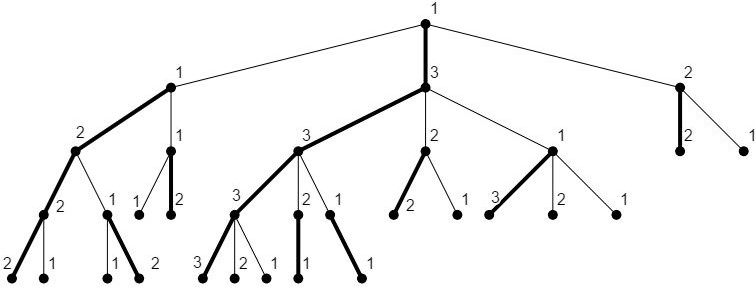
\includegraphics[height=5cm]{figures/optimal_algorithm.jpg}
	\caption{The number at each node indicates the order among siblings in which they are considered according to $S_D$.}
\end{figure}
\begin{rem}
Take a look at Figure~\ref{fig:S_D}. As the caption explains the number at each node shall demonstrate the order among children. If you take a look at the children of the root, for example, the first direction according to $S_D$ would be left, the second one would be right and last but not least the heavy child of the root would be considered.\\
It is trivial, that according to $S_D$ the heavy child of a node will always be considered at last.
\end{rem}
\begin{lem}
Let $T_1,T_2$ rooted ordered labelled trees be given. Suppose we want to compute $\delta((T_1)_v,T_2)$ with $v \in$ TopLight$(T_1)$. Then we encounter all pairs $((T_1)_u^{\circ}, (T_2)_w^{\circ})$ where $u \in T_1, w \in T_2$ and both not on the main heavy paths of $T_1, T_2$ respectively as relevant suproblems and therefore compute $\delta((T_1)_u^{\circ}, (T_2)_w^{\circ}).$ 
\end{lem}

Combining this lemma and the decomposition strategy $S_D$ leads to the following algorithm:
\begin{thm}
We compute $\delta(T_1, T_2)$ recursively as follows:
\begin{enumerate}
\item If $|V(T_1)| < |T_2|$ compute $\delta(T_2, T_1)$ instead.
\item Recursively compute $\delta((T_1)_v,T_2) \, \forall v \in$ TopLight$(T_1)$ using these recursive steps.
\item Compute $\delta(T_1, T_2)$ using the decomposition strategy $S_D$. However do not recurse into subproblems that have previously been computed in step $2$.
\end{enumerate}
Using these steps, we can compute $\delta(T_1,T_2)$ in $O(t_2^2t_1(1+\log \frac{t_1}{t_2}))$ time.
\end{thm}

\subsection{Lower bound on Decomposition Algorithms}
The potential of decomposition algorithms has a bound that has already been achieved by the previous algorithm of Demaine et al. To finish this chapter on the tree edit distance we will present a proof of a lower bound of $\Omega(t_2^2t_1)$ and illustrate the structure of trees which are used to show the actual lower bound of $\Omega(t_2^2t_1(1+\log \frac{t_1}{t_2}))$.
\begin{lem}
For any decomposition algorithm solving the tree edit distance problem,
there exists a pair of trees $(T_1,T_2)$ with sizes $t_1, t_2$ resprectively, such that the number of relevant subproblems is $\Omega(t_2^2t_1)$
\end{lem}
\begin{figure}[!ht]
	\centering
	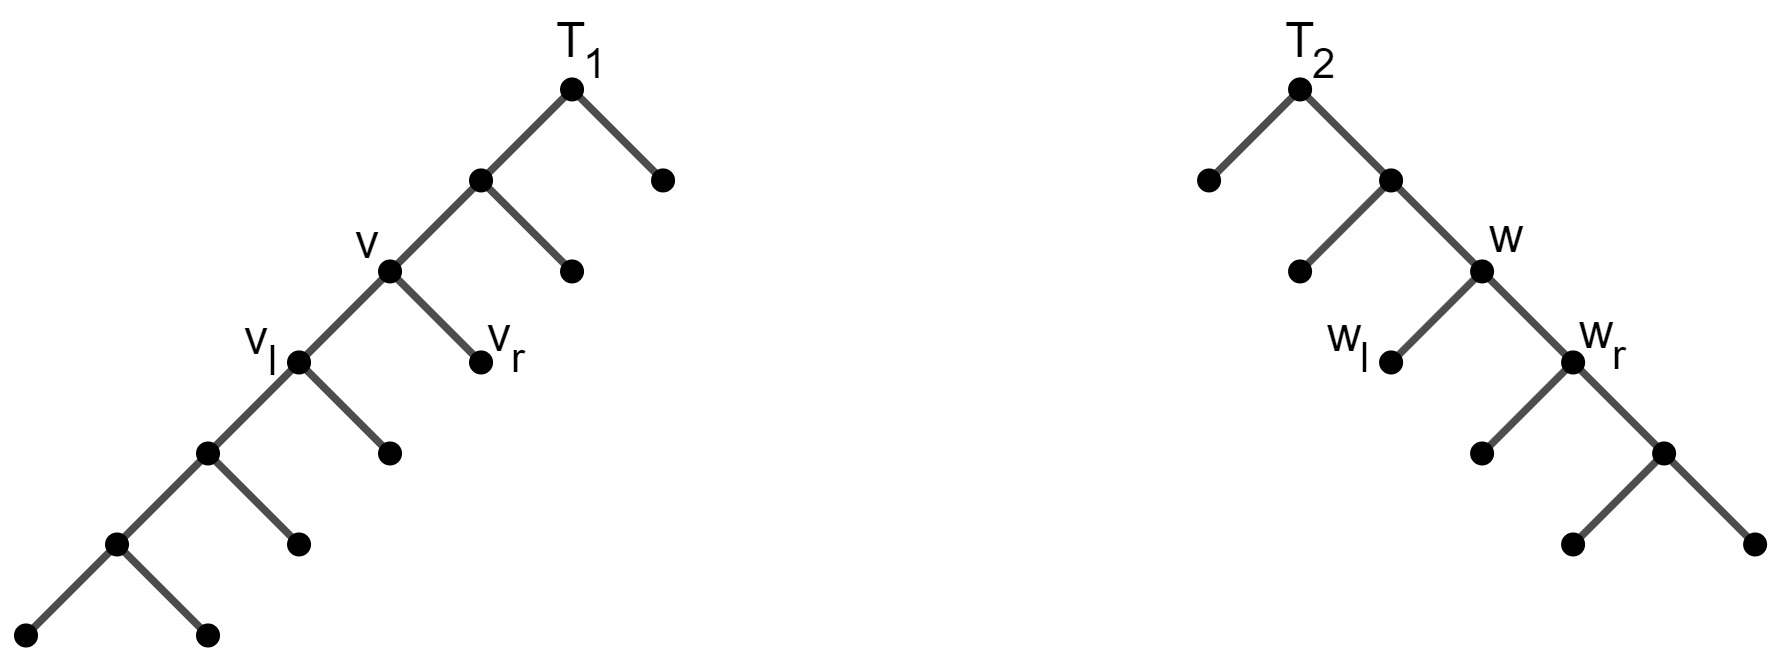
\includegraphics[height=2.5cm]{figures/O(m^2n).JPG}
	\caption{Sketch of $T_1$ and $T_2$ which fulfill a lower bound on the running time for each decomposition algorithm of $\Omega (t_2^2t_1)$}
	\label{fig:m^2n}
\end{figure}
\begin{proof}
Let $S$ be the strategy of decomposition algorithm and assume $T_1$ and $T_2$ to be as in Figure~\ref{fig:m^2n}. As previously stated, every pair $((T_1)_v^{\circ}, (T_2)_w^{\circ})$ for $v \in T_1, w \in T_2$ is a relevant subproblem for $S$. We count the number of such relevant
subproblems, where  $v$ and $w$ are inner nodes of $T_1$ and $T_2$. For an inner node $x$, let us denote the left child of $x$ as $x_l$ and the right child of $x$ as $x_r$. In the forest $(T_1)_v^{\circ}$ the rightmost root is $v_r$ and in $(T_2)_w^{\circ}$ the leftmost root is $w_l$. In each step $S$ decides the direction from which side we should delete. Every
time the strategy chooses left, we delete from $T_1$ and otherwise from $T_2$. This computational approach always keeps $v_r$ as rightmost and $w_l$ as leftmost roots of their respective forests until they are the only nodes left. So it takes at least $\min \{|(T_1)_v^{\circ}|,|(T_2)_w^{\circ}|\}$ steps until every relevant subproblem of $((T_1)_v^{\circ}, (T_2)_w^{\circ})$ is found. Since $v_r$ and $w_l$ are the outermost roots, the computational paths of $((T_1)_v^{\circ}, (T_2)_w^{\circ})$ and $((T_1)_{v'}^{\circ}, (T_2)_{w'}^{\circ})$ are completely disjoint. Because of their structure there are $\frac{t_1}{2}$
and $\frac{t_1}{2}$ internal nodes in $T_1$ and $T_2$ respectively, yielding the following equation:
$$ \sum_{(v,w) \text{internal nodes}}\min \{|(T_1)_v^{\circ}|,|(T_2)_w^{\circ}|\} = \sum_{i=1}^{\frac{t_1}{2}} \sum_{j=1}^{\frac{t_2}{2}} \min \{2i, 2j\} = \Omega(t_2^2 t_1).$$
\end{proof}
In the case of $t_2 \neq \Theta(t_1)$ this bound doesn't match the running time of Demaine et al.'s algorithm. But considering trees structured as the ones in Figure~\ref{fig:m^2nlogm/n}, one can proof the actual lower bound of  $\Omega(t_2^2t_1(1+\log \frac{t_1}{t_2}))$
\begin{figure}[]
	\centering
	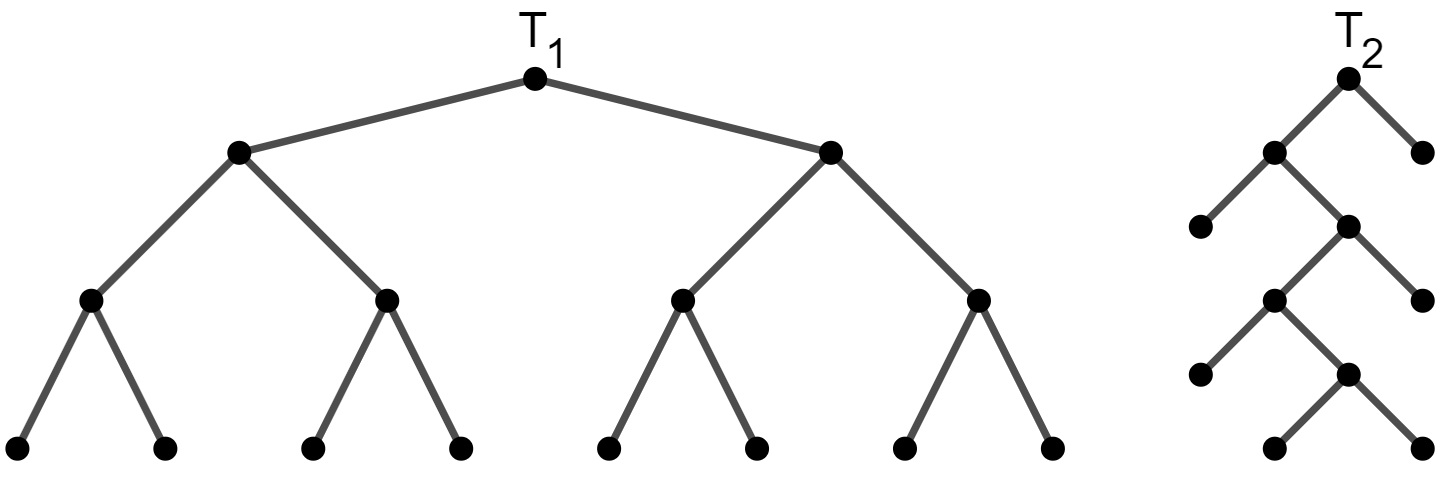
\includegraphics[height=2.5cm]{figures/O(m^2nlogn_m).JPG}
	\caption{$T_1$ and $T_2$ used to prove a lower bound of $\Omega(t_2^2t_1(1+\log \frac{t_1}{t_2}))$}
\label{fig:m^2nlogm/n}
\end{figure}
\chapter{Flexible Tree Matching}
One problem of the standard tree edit distance is the strict requirement regarding the tree parent-to-child relationship within an ordered tree, the so called hierarchy, and ordering among siblings. If a node gets mapped while computing the tree edit distance, its children have to get mapped to some descendants of this mapped node. In some domains, the most appropriate matching may not follow these requirements. One of these domains is the DOM (Document Object Model) of a website. A standard HTML-based website can easily be structured according to the respective tags. Take a look at the website in Figure~\ref{fig:website_0} and the its HTML-code in Listing~\ref{lst:DOM0}. 
\begin{figure}[!h]
    \centering
        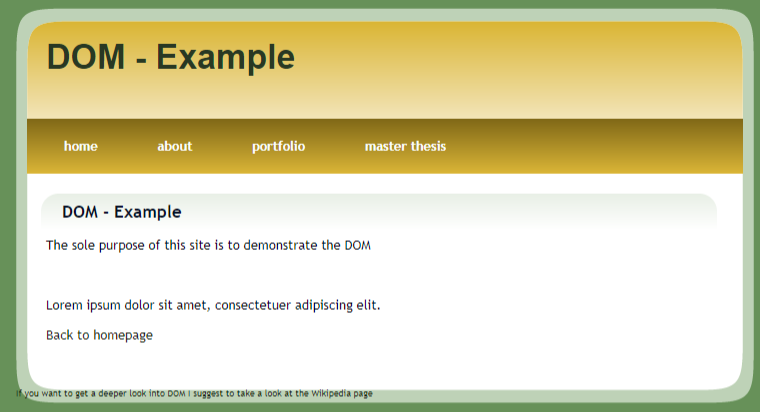
\includegraphics[width=0.60\textwidth]{figures/DOM_website.png}
        \caption{The example website.}
        \label{fig:website_0}
\end{figure} 
\lstinputlisting[language=Html, caption=Html code of DOM example, label=lst:DOM0]{figures/DOM_0.html}

The DOM-tree of the example website is intuitively clear: The outermost tag, the $<$html$>$-tag, is the tree's root. The root's children are the $<$head$>$-tag and the $<$body$>$-tag and so on. This leads to complete DOM-tree illustrated in Figure~\ref{fig:DOM_0}.
\begin{figure}[!h]
    \centering
        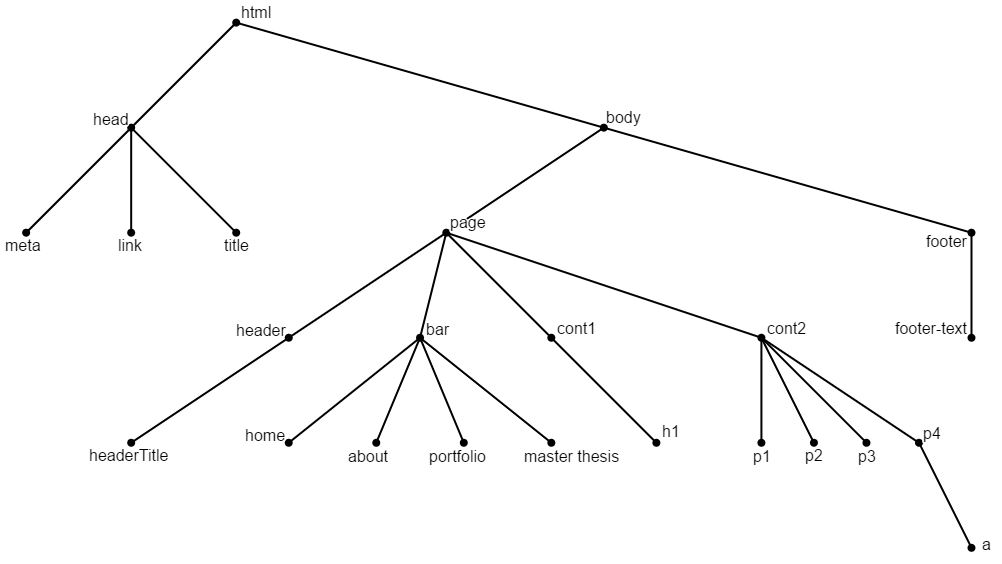
\includegraphics[width=1\textwidth]{figures/DOM_0.jpg}
        \caption{Complete DOM-tree of the example website.}
        \label{fig:DOM_0}
\end{figure}
\\
Intuitively, any small change to the website should not lead to a big distance between the two DOM-trees. Suppose one changes the order of the buttons in the header menu as well as moving one of these buttons into the content area of the website as seen in Figure~\ref{fig:website_1}. The website and its functionalities remain quite similar, but it would take about three deletions and four insertions to end up with the new DOM-tree. Obviously it would be cheaper to delete the whole header menu and therefore reduce the functionality of the website. 
\begin{figure}[!h]
    \centering
        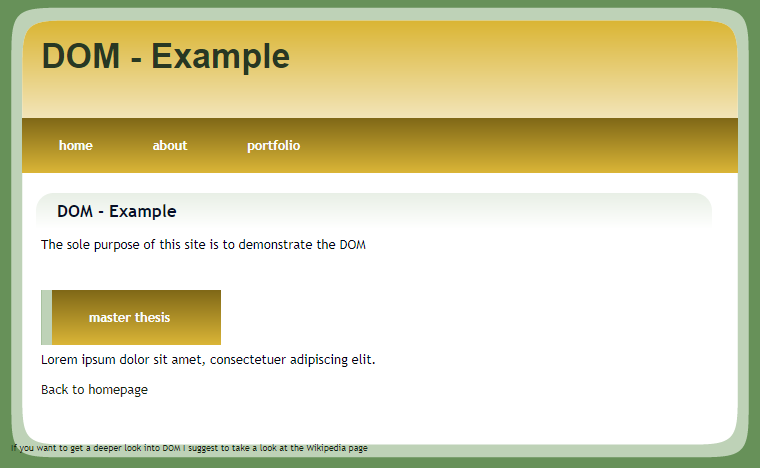
\includegraphics[width=0.60\textwidth]{figures/DOM_website_1.png}
        \caption{Small changes to the website should not affect the distance of the respective DOM-trees.}
        \label{fig:website_1}
\end{figure} 

This kind of issue arises frequently in the context of comparing tree models. Flexible tree matching models have been introduced in an effort to appropriately handle the above mentioned issues. Instead of requiring strict left-to-right ordering and hierarchy conditions, one may relax them by introducing costs to penalize the violation of this type of requirements. Kumar et al.~\cite{Kum} developed an algorithm that matches nodes with similar labels and penalizes edges that break up sibling groups or violate the hierachy. In the example above, moving the button from header menu into the content is such a violation of the hierarchy, because a node gets shifted into another subtree. This needs to have some kind of costs associated to it, but it should definitely be cheaper than deleting the subtree and inserting it again in some other place.\\
Finding the minimum flexible tree edit distance can be reduced to finding a minimum cost matching in a flexible cost model. Kumar et al. showed that finding the flexible tree edit distance is strongly $\mathcal{NP}$-complete. This implies that there are no efficient algorithms to compute the minimum flexible tree edit distance. However, there are some approximating heuristics.\\
This chapter is based on the previously cited paper by Kumar et al. 

\section{The Model for the Flexible Tree Edit Distance}
Let $T_1$ and $T_2$ be the two trees for which the flexible tree edit distances shall be computed. We construct a complete bipartite graph $G$ with\\
$G := (\{V(T_1)\cup \otimes_1\} \dot{\cup} \{V(T_2)\cup \otimes_2\}, E)$. Hence the edge set $E$ is defined as the set $E:=\{\{v_1,v_2\} \;|\; v_i \in\{V(T_i)\cup \otimes_i\}\text{ for }i =1,2\}$. The nodes $\otimes_i$ are so called \textit{no-match} nodes. Every edge $e=\{v_1,v_2\}\in E$ represents matching a node $v_1$ to a node $v_2$. If $v_2=\otimes_2$, the edge $e$ would represent the deletion of $v_1$, since $v_1$ was not matched to any node from the tree $T_2$. An analogous statement holds for an edge $\{\otimes_1,v_2\}$. Every edge $e \in T_1 \times T_2$ is assigned some cost function $c(e) = c_r(e) + c_a(e) + c_s(e)$. The exact definitions follow later. In short terms, these three summands represent the costs that we mentioned earlier in this chapter: $c_r$ represents the costs of relabelling a node, $c_a$ penalizes violations of ancestry relationships and $c_s$ punishes broken up sibling groups. Edges connecting tree nodes with no-match nodes have a fixed constant cost $w_n$, only depending on the number of nodes in the trees. The goal is to find a minimum cost flexible matching $M \subset E$ such that every node of $T_1 \cup T_2$ is covered exactly once while the no-match nodes may be covered multiple times. We call the set of all such flexible matching $M_{T_1, T_2}$.
Suppose that $v \in V(T_1)$ and $w \in V(T_2)$ and let $e:=\{v,w\}\in E$. The costs for relabelling $e$, i.e. $c_r(e)$, only depend on the nodes $v$ and $w$ themselves. They are fixed for every edge and are known before starting to match nodes. $c_a(e)$ and $c_s(e)$ on the other hand may depend on the choice of the flexible matching $M$. To be more precise the costs $c_a(\{v,w\})$ are linearly dependent on the number of children of $v$ that do not get mapped onto children of $w$. Define $M(v)\in \{T_2\cup\otimes_2\}$ to be the node that $v$ is mapped onto according to the flexible matching $M$ and suppose that $M(v) \neq \otimes_2$. Moreover, define $C(v) \subset T_1$ to be the set of children of node $v$. Then we can define $V(v)$ to be the set of children of $v$ that violate the ancestry condition, i.e.:
$$V(v) := \{v' \in C(v)\;|\;M(v') \in T_2 \setminus C(M(v))\}$$
As stated previously, the cost function $c_a(e)$ is linearly dependent on the sizes of the sets $V(v)$ and $V(w)$ with some constant factor $\omega_a$:
$$c_a(\{v,w\}) := \omega_a (|V(v)| + |V(w)|)$$
\begin{figure}[b!]
    \centering
        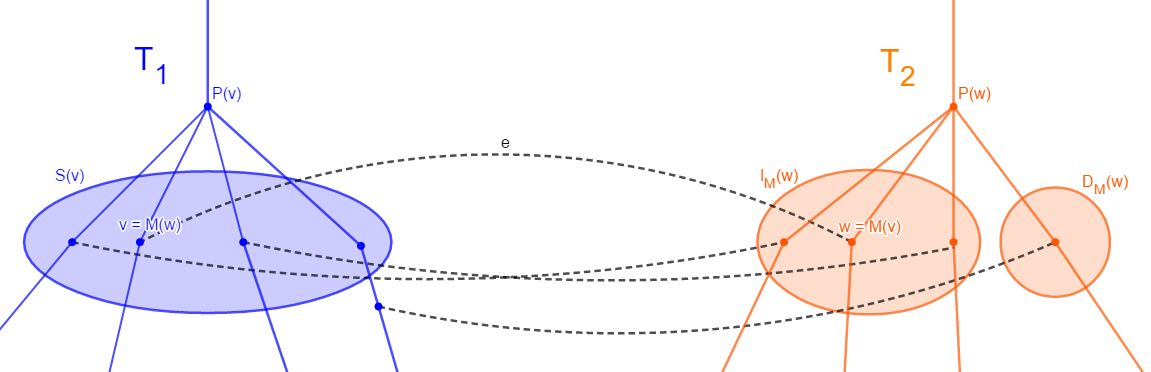
\includegraphics[width=\textwidth]{figures/Treeconcepts_flexible_tree_matching.png}
        \caption{A visual representation of the above described tree concepts.}
        \label{fig:treeConcepts}
\end{figure}
We need further tree related concepts before we can define the cost function $c_s(e)$ in a straight forward way. Therefore $P(v) \in T_1$ is defined as the parent of the node $v$ and $S(v):=C(P(v))$ is the sibling group of $v$. If $v$ is the root of the tree, then $P(v)$ does not exist and $S(v):=\{v\}$. Note that the sibling group $S(v)$ always contains the node $v$ itself and thus is not empty. For a matching $M$, we define the sibling-invariant subset of $v$, $I_M(v)$, to be the siblings of $v$ which are mapped into the same sibling group as $v$:
$$I_M(v) = \{v' \in S(v)\;|\;M(v') \in S(M(v))\}$$
Accordingly the sibling-divergent subset of $v$, $D_M(v)$, are the siblings of $v$ which are mapped to a node in $T_2 \setminus S(M(v))$:
\begin{align*}
D_M(v) :&= \{v' \in S(v)\;|\;M(v') \in T_2 \setminus S(M(v))\} \\
		&= \{v' \in S(v) \setminus I_M(v)\;|\;M(v') \neq \otimes_2\}
\end{align*}
Finally, we define the set of distinct sibling families to be the set of all sibling groups, that the siblings of $v$ map into:
$$F_M(v) = \bigcup_{v' \in S(v)} P(M(v'))$$
Now we can define the costs for sibling group violations depending on a constant $\omega_s$:
$$c_s(\{v,w\},M) := \omega_s (\frac{|D_M(v)|}{|I_M(v)||F_M(v)|} + \frac{|D_M(w)|}{|I_M(w)||F_M(w)|})$$
One can show, that the costs $c_s(\{v,w\},M)$ increase, if a node in the sibling group of $v$ or $w$ gets reassigned to some node outside of the corresponding sibling group.

\begin{defin}
Let $T_1$, $T_2$ be two rooted ordered trees. Let $G := (\{V(T_1)\cup \otimes_1\} \dot{\cup} \{V(T_2)\cup \otimes_2\}, E)$ be a graph as defined above. Furthermore let constants $\omega_n$, $\omega_a$, $\omega_s$ and the relabelling function $c_r(e)$ be given.\\
Let $M^* \in M_{T_1, T_2}$ be a flexible matching that covers each node $v \in T_i$, $i \in \{1,2\}$ exactly once and that fulfills the following equation:
$$c(M^*) := \sum_{e^* \in M^*} \, c(e^*) = \min_{M \in M_{T_1, T_2}} \sum_{e \in M} \, c(e)
$$
Then we call $c(M^*)$ the \textit{flexible tree edit distance}.
\end{defin}

\section{Approximation and Conclusion}
As spoiled in the introduction of this section, computing the flexible tree edit distance is $\mathcal{NP}$-hard. There is a short and elegant proof, that presents a reduction of the 3-partition problem to the flexible tree matching problem. Once again you can find the details in the paper of Kumar et al~\cite{Kum}. Hence, there exists no efficient algorithm that computes the flexible tree matching to optimality. But there are stochastic optimization algorithms to get an approximation of the flexible tree edit distance. Kumar et al.~\cite{Kum} presented a Monte Carlo algorithm where they fix edges one after another, prune all other incident edges to the endpoints of the current edge and update the bounds for all other nodes. They start with an empty flexible matching $M$ and calculate bounds for the values of $c_a(e)$ and $c_s(e)$ for all edges $e$. After including an edge $e_1 = \{v,w\}$ into $M$, they delete all other adjacent edges to $v$ and $w$ and update the bounds for the cost functions $c_a$ and $c_s$ for all remaining edges. Naturally the more edges are fixed, the better the bounds get. For a more detailed description of the actual algorithm, please take a look at the cited paper. The authors also described how to adapt the cost factors $\omega_r$, $\omega_s$, $\omega_a$ and $\omega_n$ step by step to improve the results.\\
Depending on the application, the flexible tree matching can have huge advantages with respect to the classic tree edit distance, especially in fields where hierarchy is suggestive rather than definitive. In different applications sibling group violations or ancestry violations may have different significance and their significance can be modelled by appropriately chosen values for coefficients $\omega_r$ and $\omega_s$. Hence the coefficients of the cost model for the flexible tree matching can be tuned so as to reflect the real life problem as accurately as possible. If you have a database of exemplar matchings you may even implement a learning cost model that improves the cost factors to follow your needs.
Nevertheless, there can not be an efficient algorithm to calculate the flexible tree edit distance. So all results are more suggestive than definitive, just like the problem itself.
\chapter{Robinson Foulds Metric}
A field, where tree edit distances get applied a lot is the field of computational biology and bioinformatics. Comparing the structure of different RNAs is a classic example of such an application. An even more important one is comparing phylogenetic trees. A phylogenetic tree or evolutionary tree is a rooted branching diagram, that shows the evolutionary connectedness of different species. Multiple species can have recent common ancestor (in the evolutionary sense). This ancestor is represented as a node with an edge to all the descended species. A leaf is called a taxon and is labelled with the species it represents. All in all, one can build one huge phylogenetic tree that represents all life on earth. For the studies of evolutionary biology, scientists often need to compare different evolutionary theories regarding a certain subset of species. Therefore they have to take a look at the structure of the corresponding subtrees and apply some distance measurement on them. \\


\section{Additional Background}
The scientific field of phylogenetics is the field of evolutionary relationships and history among species and groups of organisms. This common ancestry is described as a phylogenetic tree. The taxons, the labels of the leaves of the phylogenetic tree, are hereby the species currently investigated. The interior nodes represent some common ancestor of the investigated species. If we create a rooted phylogenetic tree, then the root would be the common ancestor of all these species. Sometimes the structure can't be fully resolved. This results in so called \textit{multifurcations}, interior nodes of degree higher than three. 
\begin{figure}
	\centering
	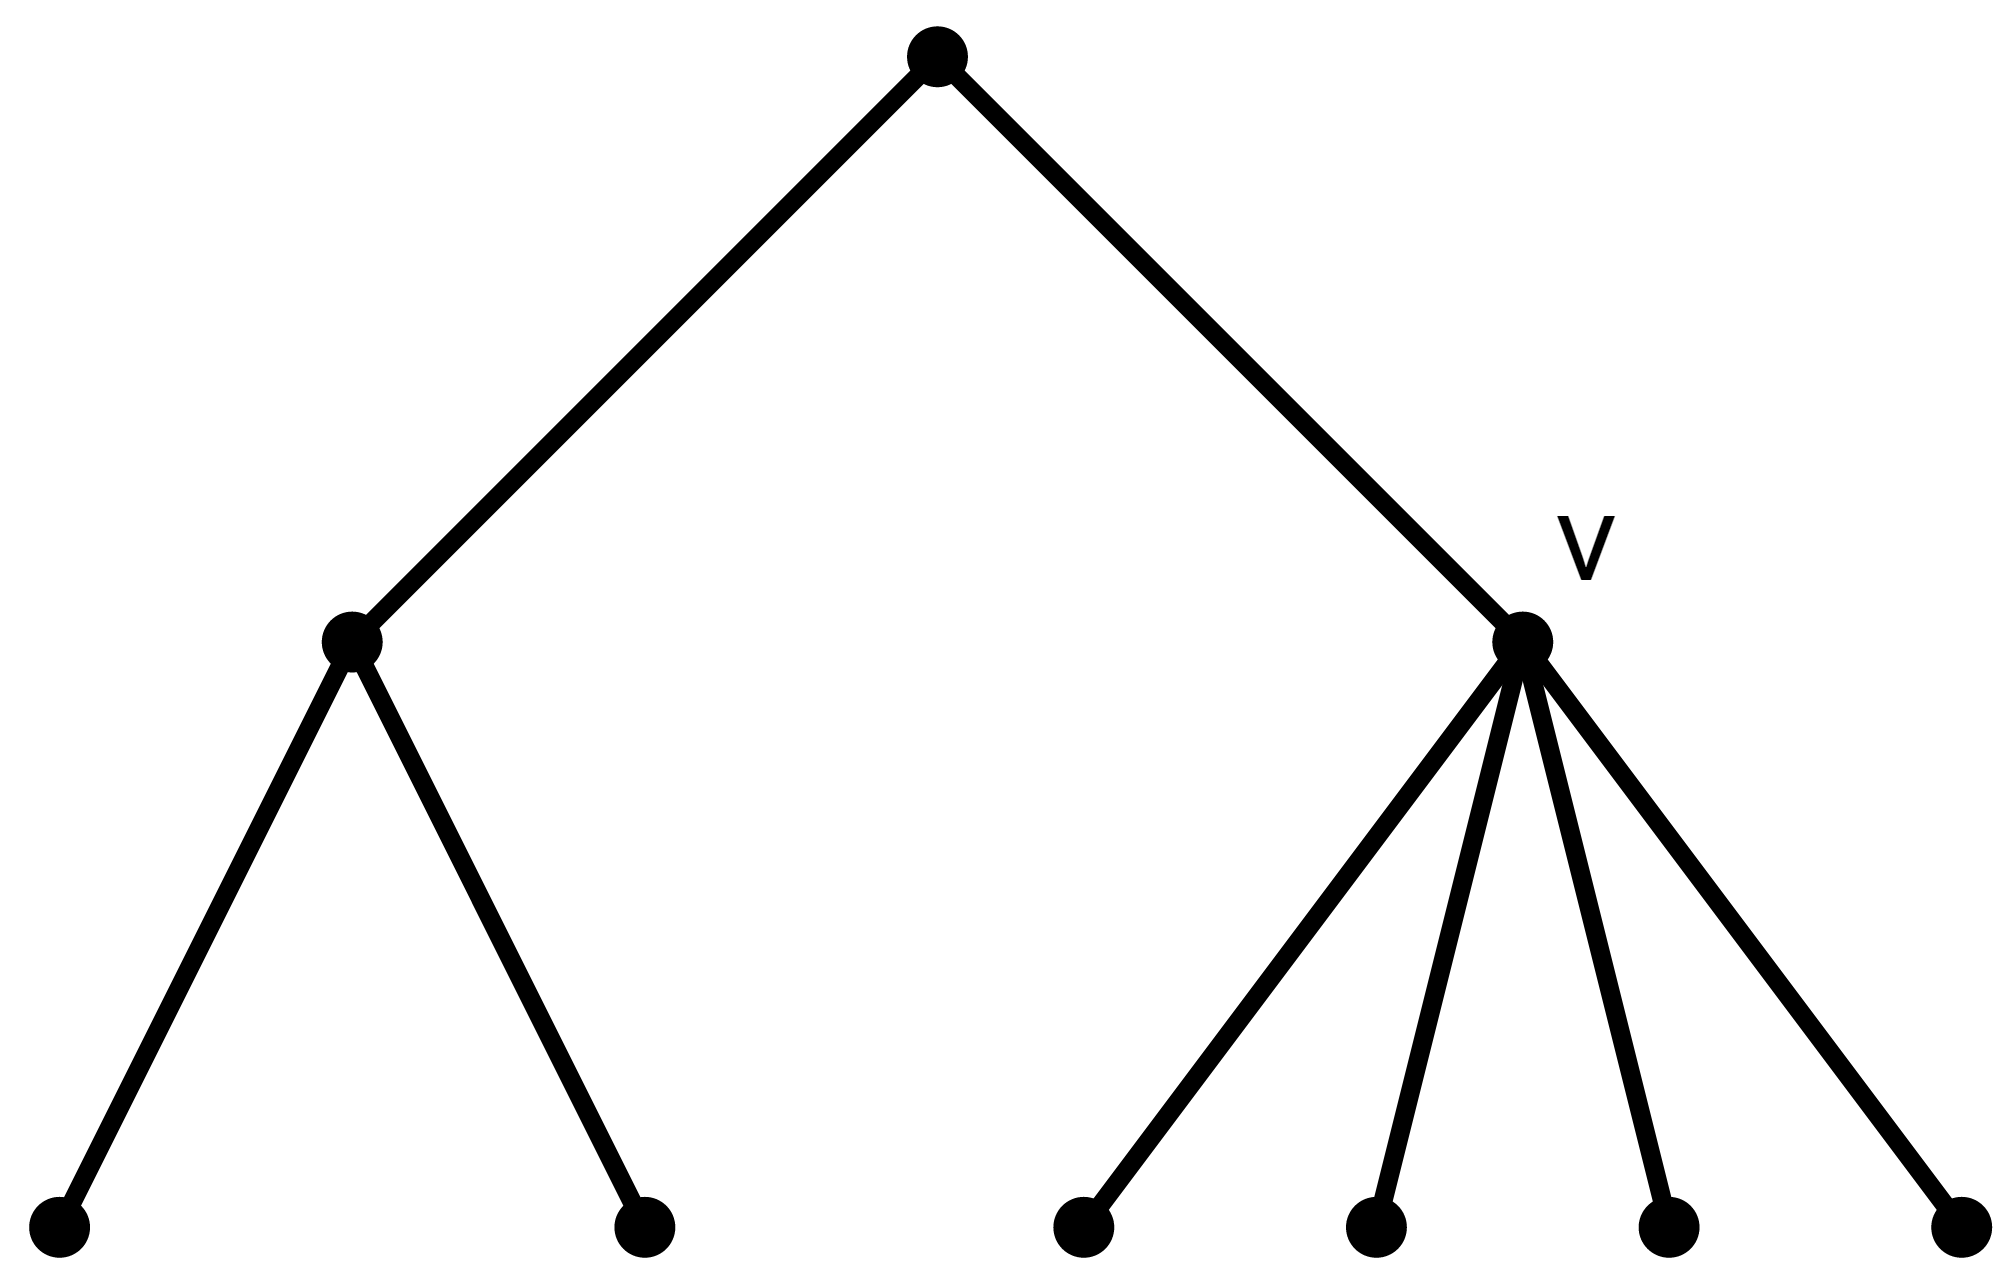
\includegraphics[width=0.4\textwidth]{figures/multifurcation.png}
    \caption{A rooted phylogenetic tree. The node $v$ is a multifurcation since its degree is larger than $3$. The ancestry relations aren't fully resolved for the children of $v$.}
\end{figure}
Multifurcations may occur due to missing data for inferring the phylogeny. Often they appear in consensus trees, when partially contradictory trees were obtained by some methods. A perfectly resolved phylogenetic tree doesn't have any multifurcations implying a binary phylogenetic tree. 

\section{The original metric}
The most commonly used distance measurement was introduced by Robinson and Foulds []. They introduced the term clade, which describes a group of leaves that have a common ancestor which they do not share with any other node.

The Robinson-Foulds metric is quite intuitive and easy to compute. It is the average number of non-trivial clades that are present in exactly one of the two trees:
\begin{defin}
Let $T_1,T_2$ be two trees with the same set of taxa $X$. Then we define the Robinson-Foulds metric $d_{RF}$ as follows:
\[ d_{RF} := \frac{1}{2}|\mathcal{C}^*(T_1) \bigtriangleup \mathcal{C}^*(T_2)| \]
\end{defin}
\begin{rem}~\label{rem:n-2clades}
Assuming that two trees $T_1$,$T_2$ have the same set of taxa $X$ with $n:= |X|$ implies that the number of interior nodes is bounded by $n-1$ for both trees. Furthermore, since we ignore trivial clades, the clade $X$, induced by the tree's root, will be ignored. Thus we end up with a maximum RF-distance of $n-2$ for two trees with the same taxa sets of size $n$.
\end{rem}
Although the Robinson-Foulds metric is commonly used, it has some well known downsides. For example changing the position of a single leaf can yield a new tree having maximal distance from the original one. Let's take a look at Figure~\ref{fig:maxRFdist}. Let $T_1$ be the top left tree and $T_2$ be the top right one. It is easy to see that the set of clades are the following:
\begin{align*}
\mathcal{C}^*(T_1) &=\{ \{1,...,j\}\;|\;j\in \{2,...,7\}\} \\
\mathcal{C}^*(T_2) &=\{ \{2,...,j\}\;|\;j\in \{3,...,7\}\} \cup \{1,8\}
\end{align*}
Obviously in tree $T_1$ every clade contains both nodes $1$ and $2$. On the other hand in tree $T_2$ every clade either contains node $1$ or $2$, but never both of them. This implies that 
\begin{align*}
\mathcal{C}^*(T_1) \cap \mathcal{C}^*(T_2) &= \emptyset \\
d_{RF} = \frac{1}{2}|\mathcal{C}^*(T_1) \bigtriangleup \mathcal{C}^*(T_2)| &= \frac{1}{2}(|\mathcal{C}^*(T_1)| + |\mathcal{C}^*(T_2)|) \\
d_{RF} = \frac{1}{2}(6 + 6) = 6
\end{align*}
However the third tree $T_3$ also has the same RF distance of $6$ to both trees $T_1$ and $T_2$. This points to another big disadvantage of the Robinson Foulds distance. The distribution of the distances is very much concentrated on the upper end of the scale. Two arbitrary phylogenetic trees with $n$ leaves on the same set of taxa have a high probability to have a Robinson Foulds distance of $n-2$. Furthermore the example shows that the Robinson Foulds distance does not compare the structure of the two trees. Otherwise the distance between $T_1$ and $T_2$ would be much smaller than the one to the tree $T_3$. 
\begin{figure}[ht!] \label{fig:maxRFdist}
    \begin{subfigure}[b]{0.45\textwidth}
        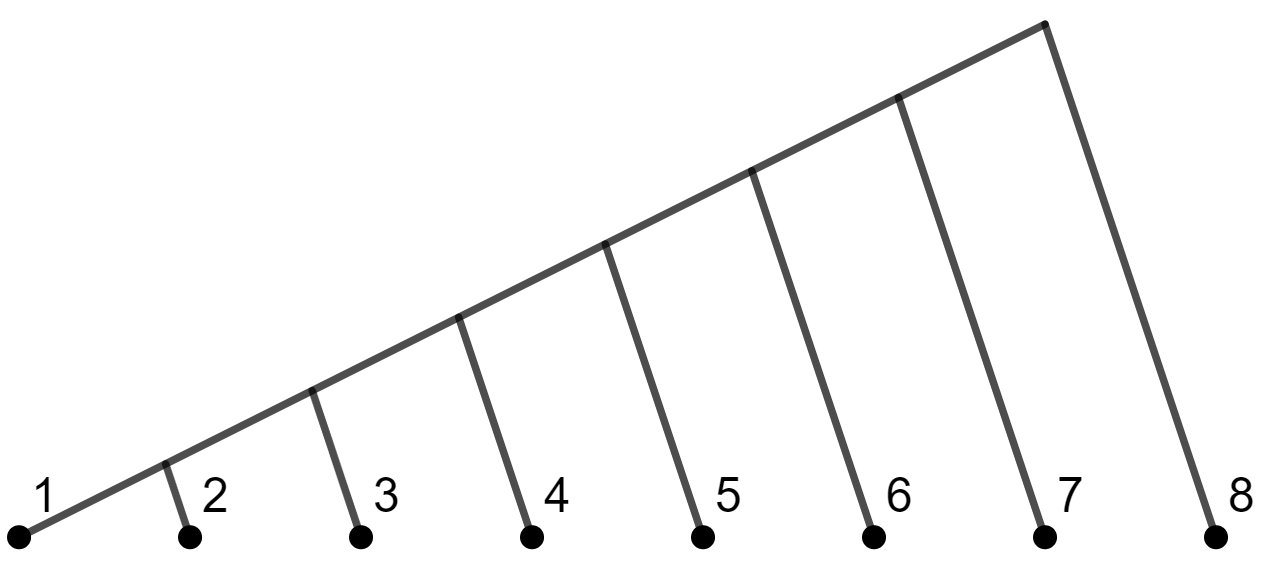
\includegraphics[width=\textwidth]{figures/RF_tree1.jpg}
    \end{subfigure}
    \quad
    \begin{subfigure}[b]{0.45\textwidth}
        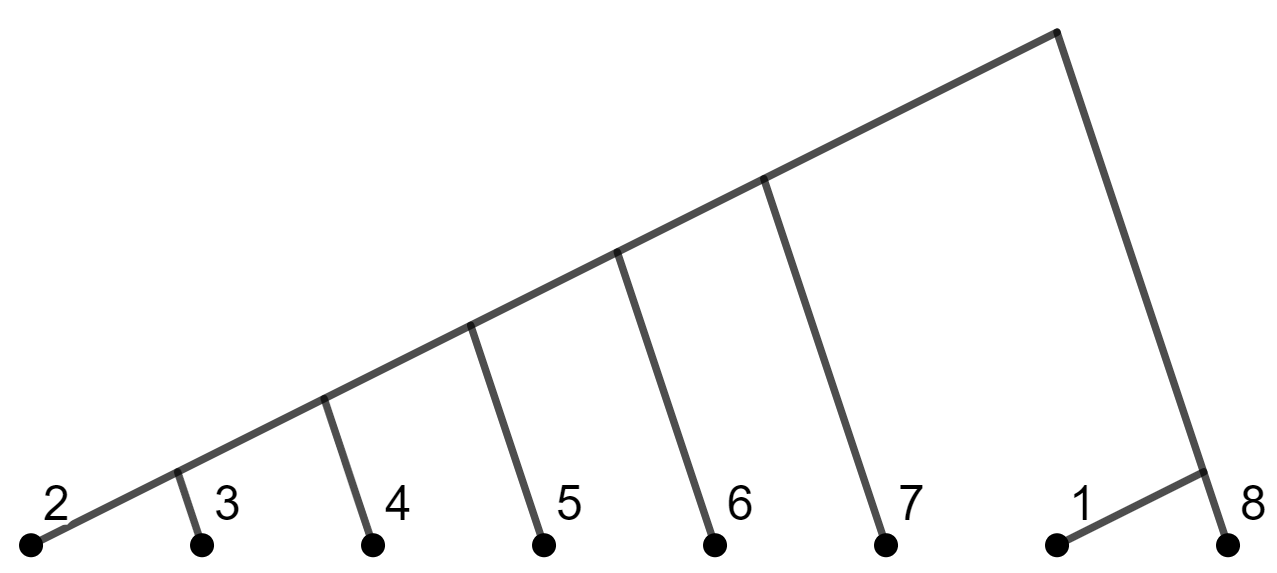
\includegraphics[width=\textwidth]{figures/RF_tree2.jpg}
    \end{subfigure}
    \quad
    \begin{subfigure}[b]{0.45\textwidth}
        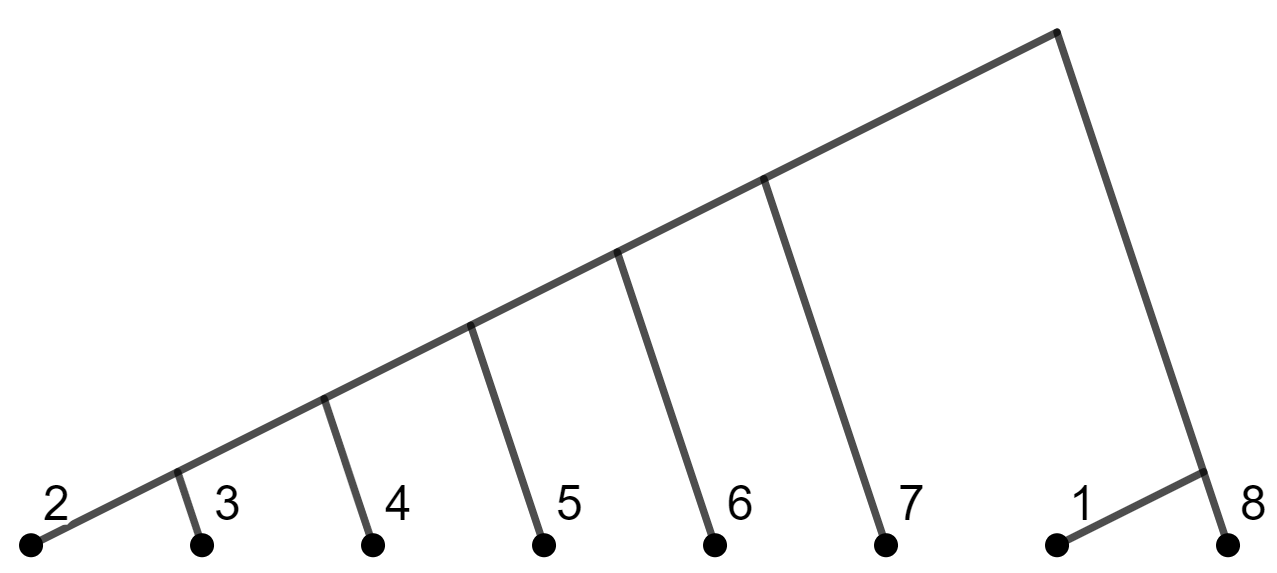
\includegraphics[width=\textwidth]{figures/RF_tree2.jpg}
    \end{subfigure}
    \caption{Three trees having the maximal RF-distance on the set of taxa $\{1,...,8\}$}
\end{figure}
 
\section{The Generalized Robinson Foulds}
To take advantage of structural similarities between $T_1$, $T_2$ Böcker et al.~\cite{Boe} suggested to extend the Robinson Foulds metric. They wanted to relax the condition of counting any clade which appears in the set of clades for one but not both trees. Therefore they introduced a bipartite graph $G(T_1, T_2)$ depending on the two trees under consideration. 
\begin{defin} \label{def:RFGraph}
Let $T_1, T_2$ be two phylogenetic trees with the same number of leaves $n$ and on the same set of taxa $X$. We define the complete bipartite graph $G_{T_1,T_2}$ on the following set of nodes:
$$G_{T_1,T_2}: \, \mathcal{C}^*(T_1) \times \mathcal{C}^*(T_2)$$
\end{defin}
\begin{defin}\label{def:RFcostfct}
Let $T_1, T_2$ be two phylogenetic trees with the same number of leaves $n$ and on the same set of taxa $X$. We introduce a cost function $\delta$ as follows:
$$\delta: \mathcal{P}(X) \times \mathcal{P}(X) \mapsto \mathcal{R}_{\geq 0} \cup \{\infty\}$$
where $\mathcal{P}(X)$ denotes the power set of $X$. The value $\delta(C,C')$ determines the dissimilarities between two clades $C$, $C' \subset X$. The value of $\delta(C, \emptyset) > 0$ denotes the dissimilarity bewtween a clade $C \in \mathcal{C}^*(T_1)$ with the empty clade in $\mathcal{C}^*(T_2)$. The value $\delta(\emptyset, C')$ is defined analogously.
\end{defin}
\begin{defin}\label{def:preRFdist}
Let $T_1, T_2$ be two phylogenetic trees with the same number of leaves $n$ and on the same set of taxa $X$. Let $G_{T_1,T_2}$ and a cost function $\delta$ be given as defined in Definitions~\ref{def:RFGraph} and~\ref{def:RFcostfct}. Furthermore let $M \subset \mathcal{C}^*(T_1) \times \mathcal{C}^*(T_2)$ be a matching in $G_{T_1,T_2}$. 
We call a clade $C \in \mathcal{C}^*(T_1)$ unmatched, if $(C, C') \notin M \; \forall C' \in \mathcal{C}^*(T_2)$, analogously for clades of $T_2$.\\
Now we can define the costs $d_{\delta}(M)$ of a matching $M$ as:
$$d_{\delta}(M) := \sum_{(C, C') \in M} \, \delta(C,C') + \sum_{\substack{C \in \mathcal{C}^*(T_1),\\ C\text{ unmatched in }M}} \delta(C, \emptyset) + \sum_{\substack{C' \in \mathcal{C}^*(T_2),\\C'\text{ unmatched in }M}} \delta(\emptyset, C')$$
Minimizing over all matchings in $G_{T_1,T_2}$ yields $\overline{d}_{\delta}(T_1,T_2)$:
$$\overline{d}_{\delta}(T_1,T_2) := \min_{M \text{ matching in }G_{T_1,T_2}} \, d_{\delta}(M)$$
\end{defin}
\begin{lem}
Let $T_1, T_2$ be two phylogenetic trees with the same number of leaves $n$ and on the same set of taxa $X$. There is a distance function $\delta_{RF}$ s.t. 
$$\overline{d}_{\delta_{RF}}(T_1,T_2) = d_{RF}(T_1,T_2)$$ 
\end{lem}
\begin{proof}
Let $\delta_{RF}: \mathcal{P}(X) \times \mathcal{P}(X) \mapsto \mathcal{R}_{\geq 0} \cup \{\infty\}$ be given as follows:
$$\delta_{RF}(C, C') = 
\begin{cases}
	0 & \text{if } C = C' \\
	\frac{1}{2} & \text{if } C = \emptyset \text{ or } C' = \emptyset \\
	\infty & \text{if } C \neq C' \text{ and } C \neq \emptyset \neq C'
\end{cases}$$
Let $M^* \subset \mathcal{C}^*(T_1) \times \mathcal{C}^*(T_2)$ be a matching s.t.:
$$\overline{d}_{\delta}(T_1,T_2) = \min_{M \text{ matching in }G_{T_1,T_2}} \, d_{\delta}(M) = d_{\delta}(M^*)$$
Since the empty matching has a finite value, $M^*$ must not contain any edge $(C, C')$ s.t. $\delta_{RF}(C, C') = \infty$. Therefore $M^*$ only contains edges where the respective clades are congruent. Thus $M^*$ minimizes the number of unmatched clades, counts them and divides this number by $2$. Thus:
$$\overline{d}_{\delta_{RF}}(T_1,T_2) =  \frac{1}{2}|\mathcal{C}^*(T_1) \bigtriangleup \mathcal{C}^*(T_2)|  = d_{RF}(T_1,T_2)$$ 
\end{proof}
\begin{lem}\label{lem:costfct}
Let $T_1, T_2$ be two phylogenetic trees with the same number of leaves $n$ and on the same set of taxa $X$. Let $G_{T_1,T_2}$ and a cost function $\delta$ be given as defined in Definitions~\ref{def:RFGraph} and~\ref{def:RFcostfct}. The task of computing the matching $M^*$ that satisfies $\overline{d}_{\delta}(T_1,T_2) = d_{\delta}(M^*)$ can be simplified by the following model:\\
For any edge $(C, C') \in E(G_{T_1,T_2})$ let its weight be given by
\begin{equation} \label{eq:costfct}
\omega(C,C') := \delta(C,\emptyset) + \delta(\emptyset, C') - \delta(C,C').
\end{equation}
Finding a minimal cost matching $M$ of clades is now equivalent to finding a maximal cost matching $M^*$ in $G_{T_1, T_2}$. \\
Furthermore, if $\delta$ is a metric, all weights are non-negative.
\end{lem}
\begin{proof}
Let $M^*$ be a maximal cost matching in $G_{T_1, T_2}$. Then the following implications are trivial:
\begin{gather*}
\sum_{\{C,C'\} \in M^*} \, \omega(C, C') = \max_{M} \, \sum_{\{C,C'\} \in M} \delta(C,\emptyset) + \delta(\emptyset, C') - \delta(C,C') \\
= \max_{M} \, \underbrace{\sum_{C \in \mathcal{C}^*(T_1)} \delta(C,\emptyset)}_{\textit{const. }K_1} - \sum_{\substack{C \in \mathcal{C}^*(T_1),\\ C\text{ unmatched}}} \delta(C,\emptyset) + \underbrace{\sum_{C' \in \mathcal{C}^*(T_2)} \delta(\emptyset, C')}_{\textit{const. }K_2} \\
- \sum_{\substack{C \in \mathcal{C}^*(T_1),\\ C\text{ unmatched}}} \delta(\emptyset, C') - \sum_{\{C,C'\} \in M} \delta(C,C')\\
= K_1 + K_2 + \max_{M} - \bigg( \sum_{\substack{C_1 \in \mathcal{C}^*(T_1),\\ C\text{ unmatched}}} \delta(C, \emptyset) + \sum_{\substack{C \in \mathcal{C}^*(T_1),\\ C\text{ unmatched}}} \delta(\emptyset, C') + \sum_{\{C,C'\} \in M} \delta(C,C') \bigg)\\
= K_1 + K_2 - \min_{M} d(M) = K_1 + K_2 - d(M^*)
\end{gather*}
Additionally, if $\delta$ is a metric, the triangle inequality holds true. Thus all all weights are non-negative.
\end{proof}
Let's compute the distances defined in Definition~\ref{def:RFcostfct}of the trees $T_2, T_2$ from Figure~\ref{fig:preRFdist} with respect to the costs of the symmetric difference between sets:
$$\delta_{sym}(C, C') = |C \triangle C'| = |C \cup C'| - |C \cap C'|$$
In this case, the best way to match a clade $\{1,...,j\} \in \mathcal{C}^*(T_1), j \geq 3$ to a clade in $\mathcal{C}^*(T_2)$ is to match it with the clade $\{2,...,j\}$, since its symmetric difference is only $1$. This handles all cases except for the clade $\{1,2\} \in \mathcal{C}^*(T_1)$ and $\{1,8\} \in \mathcal{C}^*(T_2)$. Matching those two clades is better than keeping them unassigned, since:
$$\delta_{sym}(\{1,2\},\{1,8\}) = 2 < 4 = \delta_{sym}(\{1,2\},\emptyset) + \delta_{sym}(\emptyset, \{1,8\})$$
Resulting in a matching of overall costs of $8$. 

Another way to compute the distance is to use Lemma~\ref{lem:costfct}. In Figure~\ref{fig:maxCostMatch} we can investigate the graph $G_{T_1,T_2}$ with the corresponding edge weights.
\begin{figure}
	\centering
	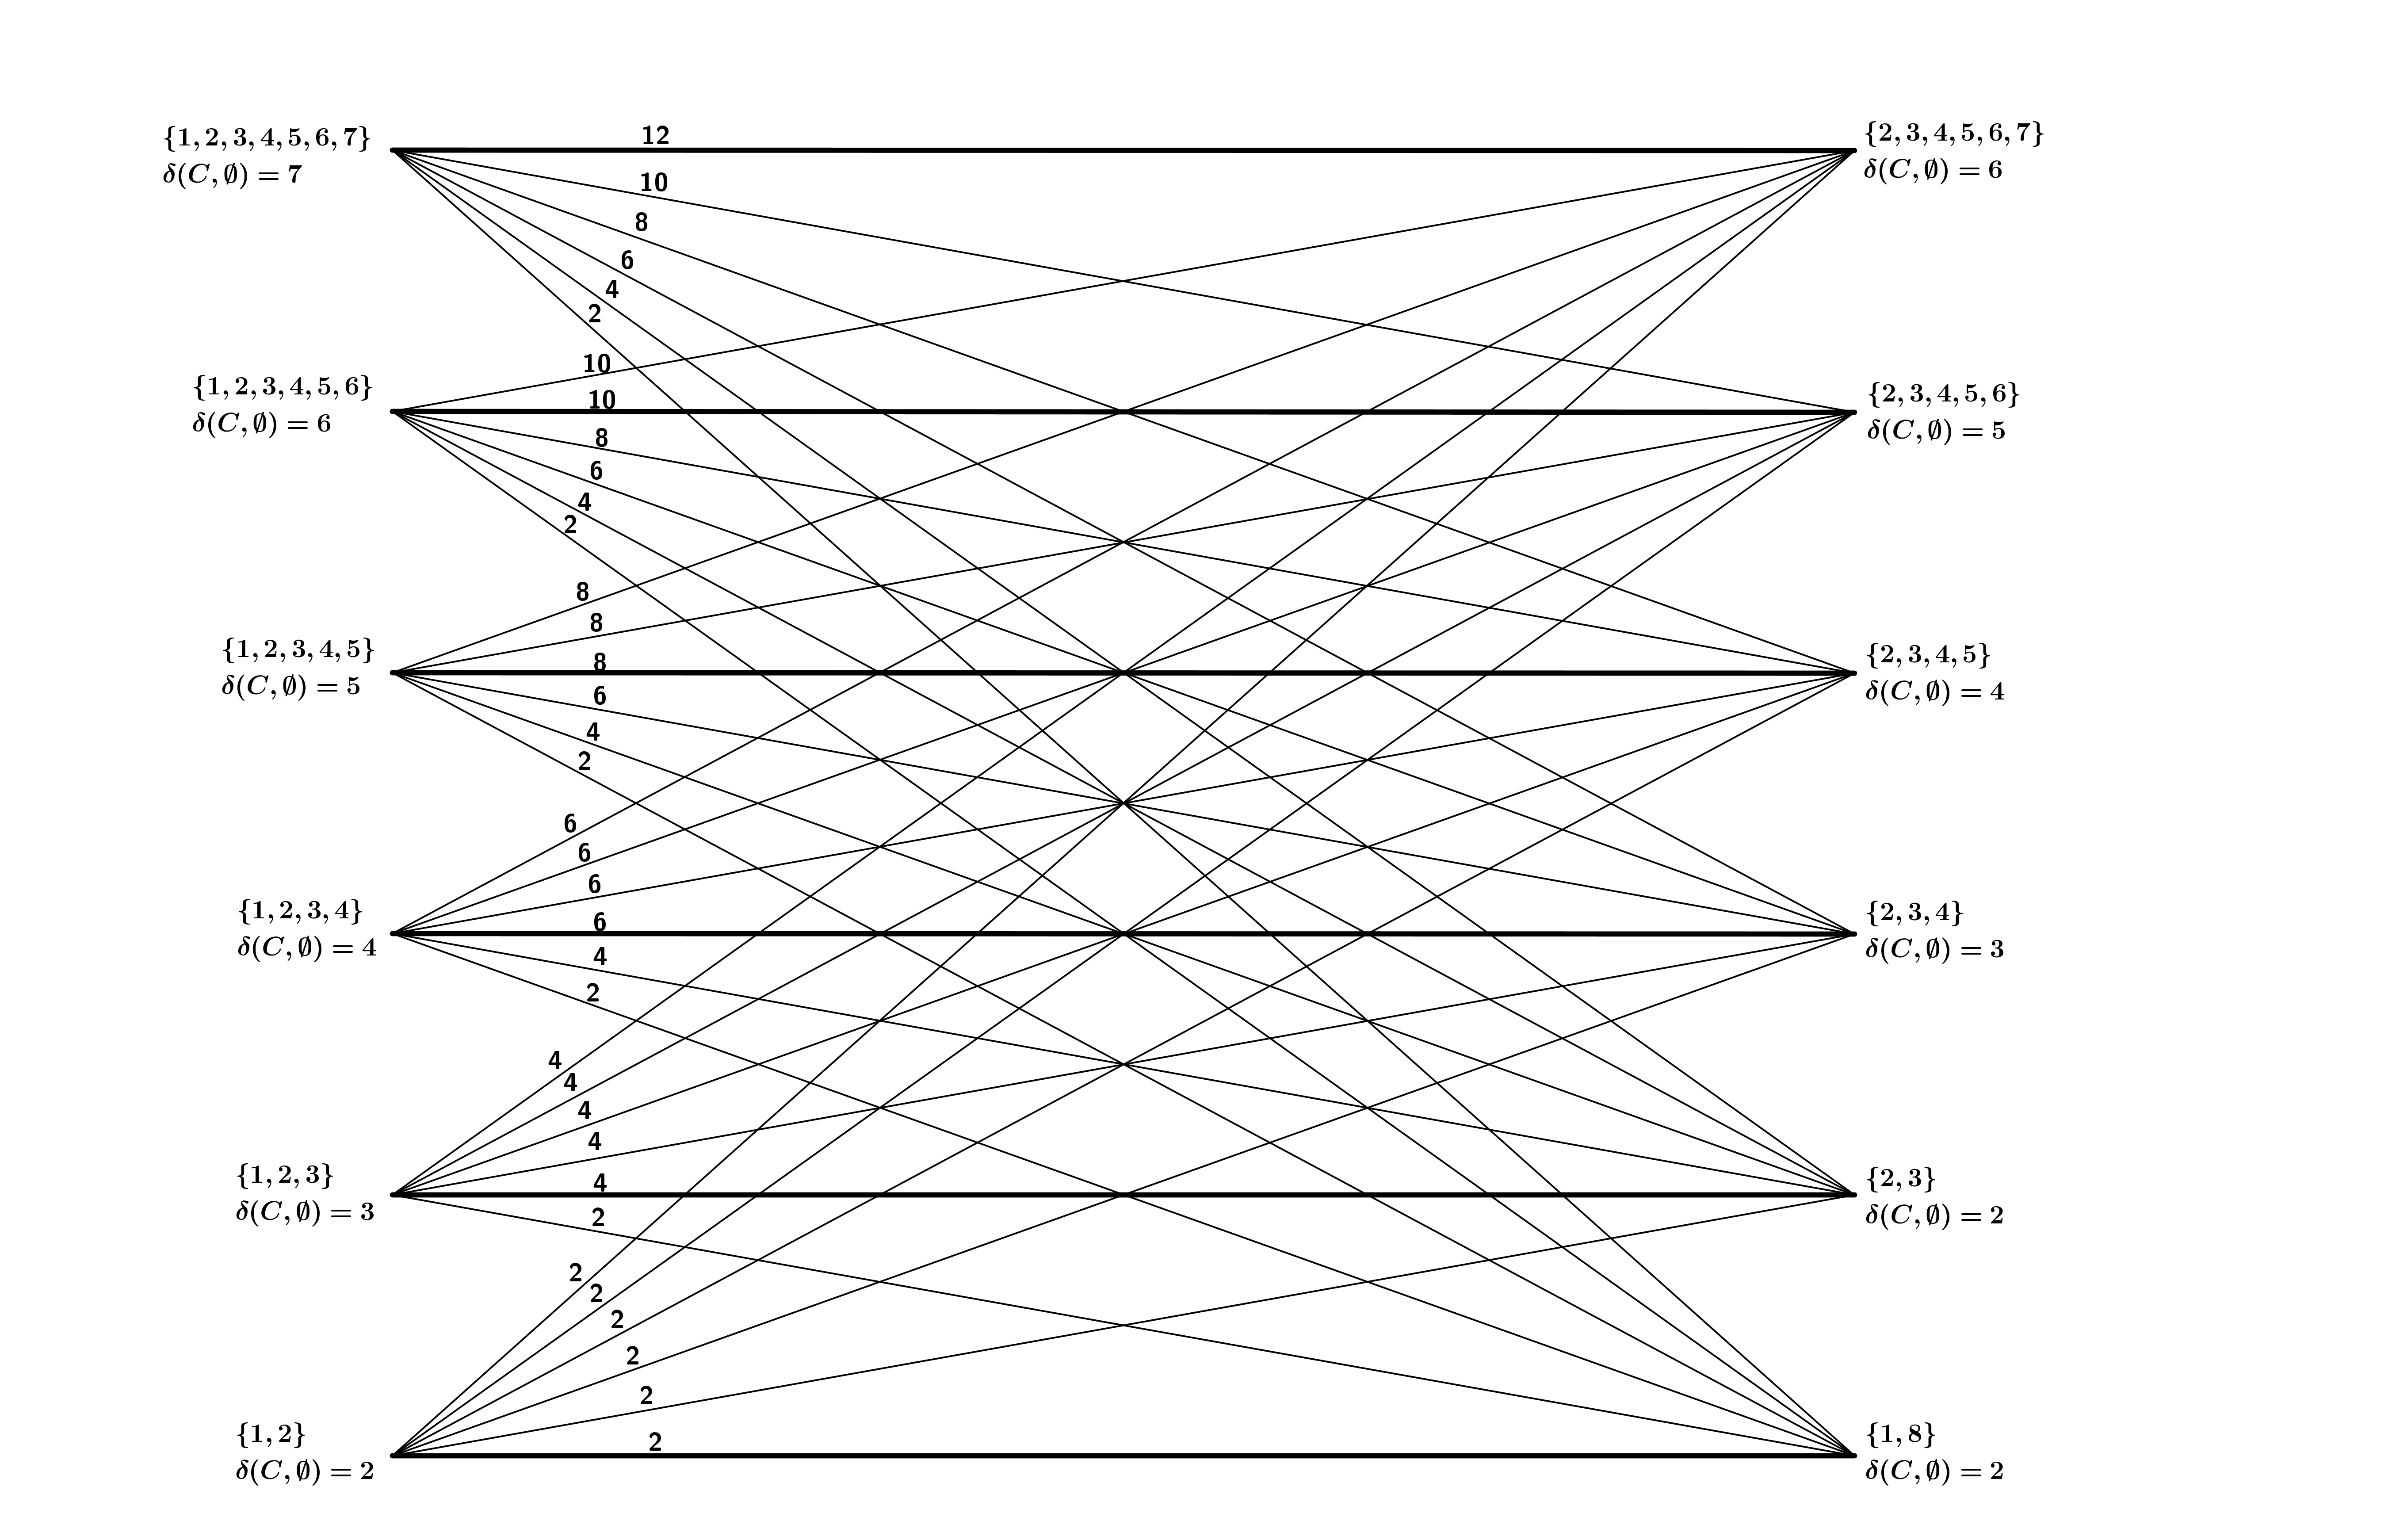
\includegraphics[width=1.25\textwidth]{figures/maxCostMatching.png}
    \caption{This is the graph $G_{T_1,T_2}$. On the left hand side we see nodes corresponding to the non-trivial clades of $T_1$, on the right hand side nodes corresponding to the ones of $T_2$. The edges of $G_{T_1,T_2}$ have their weights assigned. The maximum cost matching $M^*$ is represented by the bold edges.}
\end{figure} 
The optimal matching in $G_{T_1,T_2}$ can be seen very easily. For every edge $(C_1,C_2)$ in the matching $M^*$, the weight $\omega(C_1,C_2)$ is maximal among all edges starting at $C_1$. Thus $M^*$ indeed is optimal.

Now let's compare this distance to the distance of $T_1$ and $T_2$ to $T_3$ respectively:
\begin{align*}
\bar{d}_{\delta_{sym}}(T_1, T_2) &= 8\\
\bar{d}_{\delta_{sym}}(T_1, T_3) &= 19\\
\bar{d}_{\delta_{sym}}(T_2, T_3) &= 16
\end{align*}
This distance measure delivers values which are nearer to the observers intuitive answers. The distances indicate significant similarities between the trees $T_1$ and $T_2$. Furthermore they point out that $T_3$ has a completely different structure than the other trees.\\
Of course the values can only be compared with distances with respect to the same cost function $\delta$. Generally, comparing the distances $\overline{d}_{\delta}(T_1,T_2)$ and $\bar{d}_{\delta'}(T_1,T_2)$ is not unfeasible without adding any context. For example comparing $\bar{d}_{\delta_{RF}}(T_1,T_2) = 6 < 8 = \bar{d}_{\delta_{sym}}(T_1, T_2)$ doesn't yield any information. However one can get information from the follwoing inequalities:
\begin{align*}
6 = \delta_{RF}(T_1,T_2) = \delta_{RF}(T_1,T_3) =\delta_{RF}(T_2,T_3) = 6 \\
8 = \bar{d}_{\delta_{sym}}(T_1, T_2) < 16 = \bar{d}_{\delta_{sym}}(T_2, T_3) < \bar{d}_{\delta_{sym}}(T_1, T_3) &= 18
\end{align*}
The minimum matching for $\bar{d}_{\delta_{sym}}(T_1, T_2)$ shown above demonstrates a problem with this straight forward approach: The clade $\{1,2\} \in \mathcal{C}^*(T_1) \subset \{1,...,j\} \in \mathcal{C}^*(T_1) \forall j \geq 3$, however this doesn't hold for its matched clade $\{1,8\}$. Therefore we need to concentrate on arboreal matchings:

\begin{defin}\label{def:arboreal}
Let two rooted phylogenetic trees $T_1, T_2$ on the same set of taxa $X$ be given. A matching $M$ on their sets of non-trivial clades is called \textit{arboreal} if for any two edges $\{C_1,C_2\}, \{C_1',C_2'\} \in M$ one of the following cases hold:
\begin{enumerate}
\item $C_1 \subseteq C_1' \wedge C_2 \subseteq C_2'$
\item $C_1' \subseteq C_1 \wedge C_2' \subseteq C_2$
\item $C_1 \cap C_1' = \emptyset \wedge C_2 \cap C_2' = \emptyset$
\end{enumerate}
\end{defin}
\begin{defin}
Let $T_1$ and $T_2$, two rooted phylogenetic trees on the same set of taxa $X$, and a cost function $\delta$ be given. We define $d_{\delta}(T_1,T_2)$ as follows:
$$d_{\delta}(T_1,T_2) = \min_{\substack{M \text{ matching in }G_{T_1,T_2} \\ M \text{ arboreal}}} \, d_{\delta}(M)$$
We denote the value $d_{\delta}(T_1,T_2)$ as the \textit{generalized Robinson-Foulds distance} between $T_1$ and $T_2$ with respect to $\delta$.
\end{defin} 
\begin{rem}
Some notes about the generalized Robinson-Foulds distance:
\begin{enumerate}
\item From now on we will abbreviate the generalized Robinson-Foulds distance with \textbf{gRF}.
\item The gRF $d_{\delta}(T_1,T_2)$ and the previous distance measure $\overline{d}_{\delta}(T_1,T_2)$ are very similar. The only difference is, that the gRF minimizes over the arboreal matchings only.
\item The inequality $\overline{d}_{\delta}(T_1,T_2) \leq d_{\delta}(T_1,T_2)$ trivially holds.
\item Lemma~\ref{lem:costfct} also holds for the gRF $d_{\delta}(T_1,T_2)$. The proof works the same way, but instead of maximizing over all matchings, we only consider arboreal ones.
\end{enumerate}
\end{rem}
\begin{lem}
Let $X$, a set of taxa, and a cost function $\delta$ be given. Furthermore assume $\delta$ to be a metric. Then the gRF with respect to $\delta$ is a metric on the set of rooted phylogenetic trees on $X$.
\end{lem}
The proof is provided in the full version of the Böcker et al.'s paper~\cite{Boe}.

\subsection{Jaccard-Robinson-Foulds metric}
One specific metric used as a cost function is motivated by the Jaccard index of two sets: 
$$J(A,B) = \frac{|A \cap B|}{|A \cup B|}$$
Generalizing this idea leads to the Jaccard weights of order $k$:
\begin{align}\label{eq:JacWeights}
\delta_k(C_1,C_2) = 
\begin{cases}
0 & \text{if } C_1 = C_2 = \emptyset \\
1 - (\frac{|C_1 \cap C_2|}{|C_1 \cup C_2|})^k & \text{else}
\end{cases}
\end{align}
\begin{lem} \label{lem:kron}
Let $\delta_k(C_1,C_2)$ be given as defined in Equation~(\ref{eq:JacWeights}). Then $\delta_k(C_1,C_2)$ converge to the inverse Kronecker delta as $k \to \infty$:
$$\delta_k(C_1,C_2) =
\begin{cases}
0 & \text{if } C_1 = C_2 \\
1 & \text{if } C_1 \neq C_2
\end{cases}$$
\end{lem}
\begin{proof}
\textbf{Case 1}: $C_1 = C_2$.\\
\begin{align*}
\delta_k(C_1,C_2) = 1 - (\frac{\overbrace{|C_1 \cap C_2|}^{|C_1|}}{\underbrace{|C_1 \cup C_2|}_{|C_1|}})^k = 1 - (1)^k = 0 \; \forall k \in \mathbb{N}
\end{align*}
\textbf{Case 2}: $C_1 \neq C_2$
\begin{align*}
&\Rightarrow (C_1 \cup C_2) \setminus (C_1 \cap C_2) \neq \emptyset \\
&\Rightarrow |C_1 \cup C_2| > |C_1 \cap C_2| \\
&\Rightarrow \frac{|C_1 \cap C_2|}{|C_1 \cup C_2|} < 1 \\
&\Rightarrow (\frac{|C_1 \cap C_2|}{|C_1 \cup C_2|})^k \underset{k \to \infty}{\to} 0
\end{align*}
\end{proof}
\begin{defin}
Let $T_1$ and $T_2$, two rooted phylogenetic trees on the same set of taxa $X$ and a positive $k \, \in \, \mathbb{R}_{\geq 0}$ be given. The induced gRF metric is called Jaccard-Robinson-Foulds metric (\textbf{JRF}) of order $k$ and is denoted by $d_{JRF}^{(k)}(T_1,T_2)$.\\
\end{defin}
\begin{thm}
The JRF of order $k$ converges to the Robinson-Foulds distance as $k \to \infty$.
\end{thm}
\begin{proof}
For a fixed problem, there is only a finite number of non-trivial clades. Every Jaccard-distance tends to the inverse Kronecker delta as stated in Lemma~\ref{lem:kron}. Therefore the following holds:
\begin{align*}
\forall \, 0 < q < 1: \exists \, K \in \mathbb{N} \; \text{s.t.} \forall \, k > K:\\
 \delta_k(C_1,C_2) 
 \begin{cases} 
 = 0 &\text{ if }C_1 = C_2 \\
 = 1 &\text{ else if } C_1 = \emptyset \text{ or } C_2 = \emptyset\\
 > 1-q &\text{ else if } C_1 \neq C_2
 \end{cases}
\end{align*}
Let $M$ be a matching that minimizes $d_{RF}(T_1,T_2)$. 
\begin{align*}
&d_{RF}(M) - d_{JRF}^{(k)}(M) =\\
&\sum_{(C, C') \in M} \, (\delta_{RF}(C,C') - \delta_{JRF}^{(k)}(C,C')) + \sum_{\substack{C \in \mathcal{C}^*(T_1),\\ C\text{ unmatched in }M}} (\overbrace{\delta_{RF}(C, \emptyset)}^{=1} - \overbrace{\delta_{JRF}^{(k)}(C, \emptyset)}^{=1}) \\
&+ \sum_{\substack{C' \in \mathcal{C}^*(T_2),\\C'\text{ unmatched in }M}} (\overbrace{\delta_{RF}(\emptyset, C')}^{=1} - \overbrace{\delta_{JRF}^{(k)}(\emptyset, C')}^{=1}) = \\
&\sum_{\substack{(C, C') \in M \\ C = C'}} \, (\overbrace{\delta_{RF}(C,C')}^{=0} - \overbrace{\delta_{JRF}^{(k)}(C,C')}^{=0}) + \sum_{\substack{(C, C') \in M \\ C \neq C'}} \, (\overbrace{\delta_{RF}(C,C')}^{=1} - \overbrace{\delta_{JRF}^{(k)}(C,C'))}^{> 1-q} < \\
& \sum_{\substack{(C, C') \in M \\ C \neq C'}} q < n*q \underset{q \rightarrow 0}{\rightarrow} 0 
\end{align*}
\end{proof}

\subsection{Computational Complexity}
In their paper Böcker et al. demonstrate a polynomial reduction from the $(3,4)$-SAT problem to the problem of finding a minimal cost arboreal matching, even if the cost function $\delta$ is a metric. The $(3,4)$-SAT is the problem of finding a satisfying assignment for a Boolean formula in which every clause consists of exactly $3$ literals and any variable occurs $4$ times.\\
The authors of the above mentioned paper were able to construct a minimum arboreal matching instance $I$ for any Boolean formula $\phi \in (3,4)$-SAT. If the problem $I$, using the symmetric difference as cost function, admits a solution with a value smaller than a certain value, the original problem of finding a correct assignment for $\phi$ has a solution. For more details we suggest to read the original paper~\cite{Boe}. 
\begin{thm}
For an instance of the arboreal matching using the symmetric difference as cost function $\delta$ and an integer $k$, it is $NP$-complete whether there exists an arboreal matching of cost at most $k$.
\end{thm}

\subsection{An Integer Linear Program}
One way to approach an $\mathcal{NP}$-complete problem is to formulate it as an integer linear program and solve the latter. Therefore Böcker et al. set up an integer linear programming formulation to find a minimum cost arboreal matching.\\
Let two rooted phylogenetic trees $T_1 = (V_1,E_1)$ and $T_2 = (V_2,E_2)$ and a cost function $\delta: \mathcal{C}(T_1 \times \mathcal{C}(T_2) \mapsto \mathbb{R}_{\geq 0}$ be given. We number the clades in $\mathcal{C}(T_i)$ from $1$ to $|V_i|$ for $i \in \{1,2\}$. Then the indicator variable $x_{i,j}$ represents whether the $i$-th clade $C_i$ in $\mathcal{C}(T_1)$ is matched with the $j$-th clade $C'_j$ in $\mathcal{C}(T_2)$. We use the cost function introduced in Equation~(\ref{eq:costfct}) to find a minimum cost matching while maximizing the sum of the cost function. To recapitulate, the value for $\omega(C_i,C'_j)$ is:
$$\omega(C_i,C'_j) = \delta(C_i,\emptyset) + \delta(\emptyset, C'_j) - \delta(C_i,C'_j)$$
We also have to make sure that the assignment we receive satisfies the conditions for an arboreal matching. Therefore we introduce the set $\mathcal{I}$ with the following properties:
\begin{equation}\label{eq:setI}
\mathcal{I} := \bigg\{ \{(i,j), (k,l)\} \, \Big| \, \parbox{9.8cm}{The edges $(C_i, C'_j)$ and $(C_k, C'_l)$ violate the conditions
\\for arboreal matchings defined in Definition~\ref{def:arboreal}} \bigg\}
\end{equation}
\begin{thm}\label{thm:gRF_LP}
Let $T_1$ and $T_2$, two rooted phylogenetic trees on the same set of taxa $X$ with $|X|=:n$, and a cost function $\delta$ be given. Furthermore let a fixed order of all non-trivial clades in $\mathcal{C}(T_1)$ and $\mathcal{C}(T_2)$ and the cost function $\omega(C_i,C_j')$ be given. We introduce an integer linear problem (ILP) with decision variables $x_{i,j}$ as follows.
\begin{align}
\max &\sum_{i=1}^{n-2} \sum_{j=1}^{n-2} \; \omega(C_i, C'_j) x_{i,j} \label{eq:max} \\
\text{s.t.} &\sum_{j=1}^{n-2} \; x_{i,j} \leq 1 & \forall i \in \{1,...,n-2\} \label{eq:V_1} \\
&\sum_{i=1}^{n-2} \; x_{i,j} \leq 1 & \forall j \in \{1,...,n-2\} \label{eq:V_2} \\
&x_{i,j} + x_{k,l} \leq 1 & \forall \{(i,j), (k,l)\} \in \mathcal{I} \label{eq:arb} \\
&x_{i,j} \in \{0,1\} & \forall i \in \{1,...,n-2\}, \forall j \in \{1,...,n-2\} \label{eq:int}
\end{align}
Let $x^*_{i,j}$ be the values of the indicator variables $x_{i,j}$ of an optimal solution of the ILP. Let $M^*$ be the following set of edges:
$$(C_i,C_j') \, \in \, M^* \quad \Leftrightarrow \quad x^*_{i,j} = 1$$
Then the set of edges $M^*$ is a matching that realizes the value of the gRF:
$$d_{\delta}(T_1, T_2) = d_{\delta}(M^*)$$
\end{thm}
\begin{proof}Here we sketch the proof of the equivalence between the ILP~(\ref{eq:max}) - (\ref{eq:int}) and the minimum cost arboreal matching problem.\\
First and foremost, the restriction to integer decision variables in Equation~(\ref{eq:int}) ensures, that we either choose an edge to be in the matching or not. Thus we indeed get a set of edges. Furthermore Equations~(\ref{eq:V_1}) and~(\ref{eq:V_2}) restricts the chosen set of edges to be a (not necessarily complete) matching. Last but not least, because of Equation~(\ref{eq:arb}) we can be certain that the matching we end up with is a an arboreal matching, since we constructed the set $\mathcal{I}$ exactly this way. As proven in Lemma~\ref{lem:costfct}, the arboreal matching of maximum cost with respect to the cost function~(\ref{eq:max}) is an arboreal matching that minimizes the gRF $d_{\delta}(T_1, T_2)$.
\end{proof}
\begin{rem}
The number of non-trivial for a phylogenetic tree with $X$ as the set of taxa is $n-2$ as shown in Remark~\ref{rem:n-2clades}. Thus the sums in the inequalities (\ref{eq:max}),(\ref{eq:V_1}),(\ref{eq:V_2}) have an upper bound of $n-2$.\\
\end{rem}
The number of restrictions of the ILP influences the running time of any algorithm that computes or approximates an optimal solution. It is obvious, that there are $2n-4=\mathcal{O}(n)$ restrictions handling the issue of ending up with a viable matching (\ref{eq:V_1}), (\ref{eq:V_2}). \\
Computing the number of restrictions for ensuring the matching to be arboreal, Inequalities (\ref{eq:arb}), depends on the set $\mathcal{I}$. However the following lemma shows the order of the size of $\mathcal{I}$.
\begin{lem}\label{lem:numberOfRestrictions}
Let two phylogenetic trees $T_1$, $T_2$ with set of taxa $X$, $|X| =: n$, and the set $\mathcal{I}$ be given as described in Equation~(\ref{eq:setI}). Then the size of $\mathcal{I}$ is of order:
$$|\mathcal{I}| = \mathcal{O}(n^2 \log(n)^2)$$
\end{lem}
\begin{proof}
For a non-trivial clade $C^{(i)} \in \mathcal{C}(T_i)$, $i \in \{1,2\}$, we define the set of non-trivial predecessor clades as follow:
$$P(C^{(i)}) := \{C | C \in \mathcal{C}^*(T_i), C^{(i)} \subsetneq C\}$$ 
By definition every clade in $\mathcal{C}^*(T_i)$ corresponds to a node $v^{(i)}_{C^{(i)}} \in V(T_i)$. Thus every clade in the set of non-trivial predecessor clades $P(C^{(i)})$ corresponds to an inner node on the path from $v^{(i)}_{C^{(i)}}$ to the root of $T_i$.

\textbf{Claim 1}. Let $C^{(i)} \in \mathcal{C}(T_i)$, $i \in \{1,2\}$ be given, where both of them have a non-trivial predecessor: $|P(C^{(i)})| \geq 1$. Furhtermore let $C^{(i)'} \in P(C^{(i)})$ be given for $i \in \{1,2\}$. Then the following inclusion holds:
$$ \{(C^{(1)},C^{(2)'}), (C^{(1)'}, C^{(2)})\} \in \mathcal{I}$$

\textit{Proof of Claim 1}. Because of the way the non-trivial predecessors are constructed, we know that $C^{(1)} \subsetneq C^{(1)'}$ and $C^{(2)} \subsetneq C^{(2)'}$. Thus the set of edges does not fulfill the conditions (1) and (2) of the definition for arboreal matchings.

Therefore we have to count the number of such pairings to get a lower bound on the size of $\mathcal{I}$. For an inner node $v_i \in V(T_i)$ corresponding to a clade $C^{(i)}$ we define the following value:
$$p(v_i) := |P(C^{(i)}|$$ 
This value suggests how many pairings of clades within tree $T_i$ exist, where $C^{(i)}$ is the smaller clade. Furthermore we introduce the following value:
$$P(T_i) = \{ p(v) | v \in V(T_i), \, v \text{ inner node of }T_i\} $$

Let's take a look at Figure~\ref{fig:path_length}. The figure demonstrates that the value $p(v_i)$ is exactly the height of this node decreased by $1$, since the root does not count as a non-trivial predecessor. In tree $T_1$ there are overall $2$ possible pairings of a clade and a clade containing the first one, in tree $T_2$ there are 3 pairings. Using the notation above we have:
$$ P(T_1) = 2,\quad P(T_2) = 3$$
Thus overall the set $\mathcal{I}$ has to have at least $P(T_1)*P(T_2)=6$ pairings of edges as constructed in Claim 1.\\

\textbf{Claim 2}. Let $T_1$, $T_2$ be two full binary trees with the same number of leaves. Let $T_1$ be \textit{more balanced} than $T_2$, meaning:
$$ \sum_{v \in V(T_1)} \text{height}(v) < \sum_{v \in V(T_2)} \text{height}(v)$$
Then the following statement is true:
$$P(T_1) < P(T_2)$$

\textit{Proof of Claim 2}. If $T_1$ is more balanced, the same holds true for the trees induced by the inner nodes of $T_1$ and $T_2$ respectively. For an inner node $v_i$ in $T_i$, the only difference between height$(v_i)$ and the value $p(v_i)$ is, that the height counts the root of $T_i$ as well. And since the number of inner nodes are the same in both trees the following inequalities hold:
\begin{align*}
\sum_{v \in V(T_1)} \text{height}(v) &< \sum_{v \in V(T_2)} \text{height}(v)\\
\Rightarrow \sum_{v \text{ inner node of }T_1} \text{height}(v) &< \sum_{v \text{ inner node of }T_2} \text{height}(v)\\
\Rightarrow \sum_{\substack{v \text{ inner node of }T_1 \\ v \neq r_{T_1}}} \text{height}(v) + \text{height}(r_{T_1}) &< \sum_{\substack{v \text{ inner node of }T_2 \\ v \neq r_{T_2}}} \text{height}(v) + \text{height}(r_{T_2}) \\
\Rightarrow \sum_{\substack{v \text{ inner node of }T_1 \\ v \neq r_{T_1}}} (p(v)-1) &< \sum_{\substack{v \text{ inner node of }T_2 \\ v \neq r_{T_2}}} (p(v)-1)\\
\Rightarrow \sum_{\substack{v \text{ inner node of }T_1 \\ v \neq r_{T_1}}} p(v) \quad -(n-2) &< \sum_{\substack{v \text{ inner node of }T_2 \\ v \neq r_{T_2}}} p(v) \quad -(n-2)\\
\Rightarrow P(T_1) &< P(T_2) \\
\end{align*}

Let $f: \, \mathbb{N} \to \mathbb{N}$ be a function s.t. $f(n)$ is a tight lower bound on $P(T)$ for any full binary tree $T$ with $n$ leaves.

\textbf{Claim 3}. Let $k \in \mathbb{N}_{\geq 2}$. Then:
$$f(2^k) = (k-3)2^k + 4$$

\textit{Proof of Claim 3}. We make an inductive argument.
We start with the induction base where $k =2$:\\
Let $T$ be the perfectly balanced tree with $4$ leaves. As shown in Claim 2, this tree has the smallest value $P(T)$ among all full binary trees with $4$ leaves. This argument is supported by the fact that $P(T)=0$.
$$f(2^2)= (2-3)2^2 +4 = -1*4 - 4 = 0$$
\begin{figure}\label{fig:build2K}
    \begin{subfigure}[b]{0.8\textwidth}
        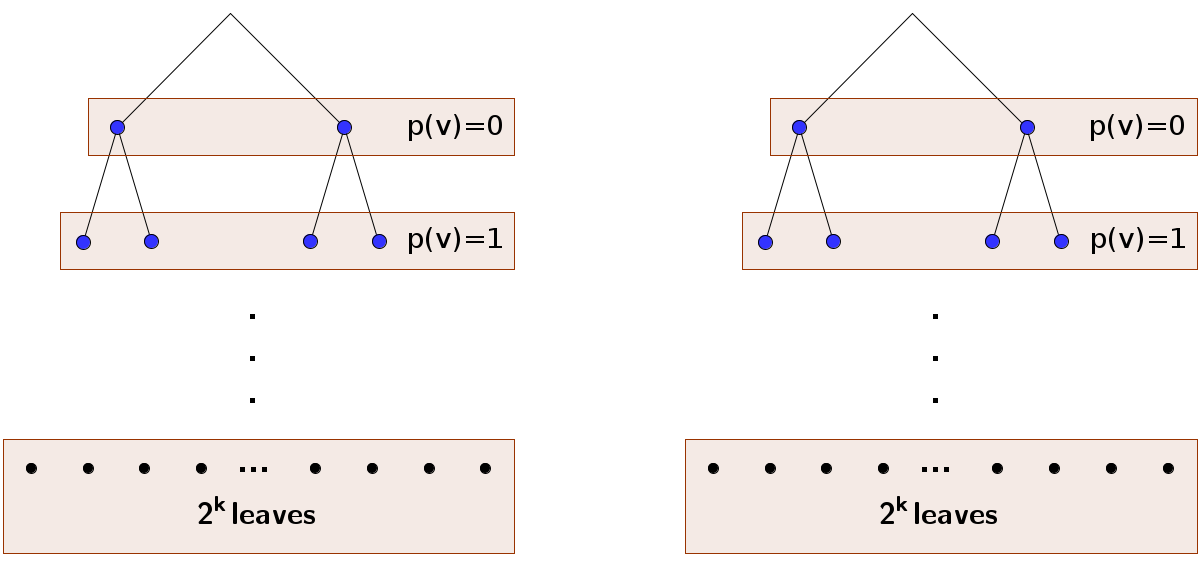
\includegraphics[width=\textwidth]{figures/2k_construction1.png}
        \caption{First we start with two perfectly balanced trees with $2^k$ leaves each.}
    \end{subfigure}
    \quad
    \begin{subfigure}[b]{0.8\textwidth}
        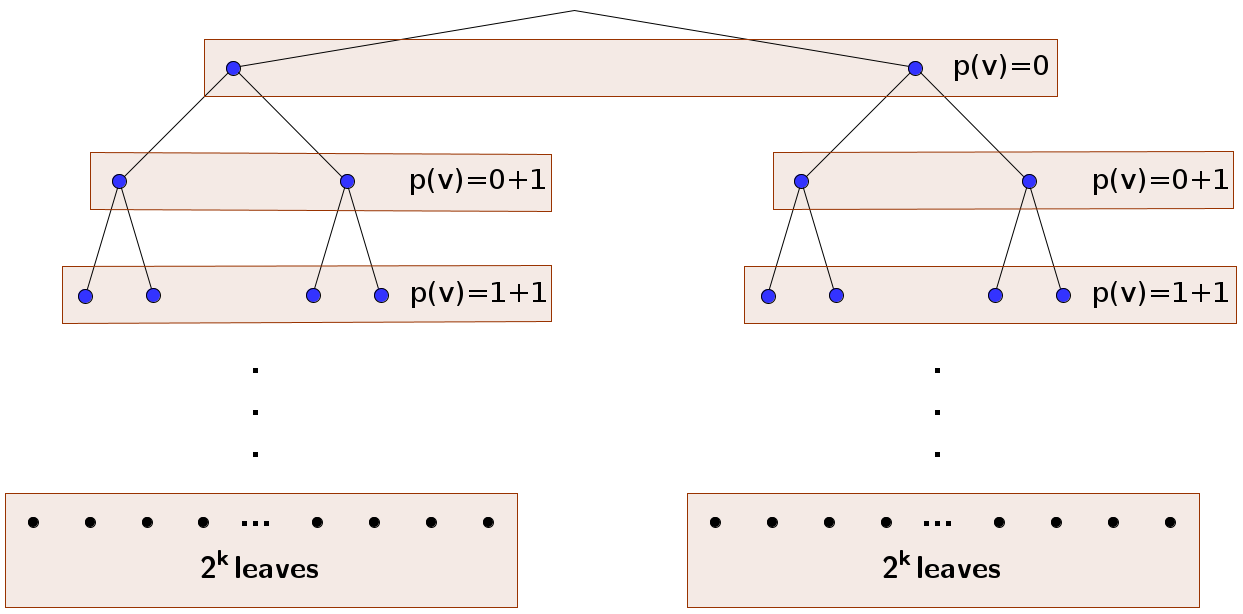
\includegraphics[width=\textwidth]{figures/2k_construction2.png}
        \caption{Now we connect them by adding a new root node and appending the roots of the trees as children.}
    \end{subfigure}
    \caption{The value of $p(v)$ increases by $1$ for all inner nodes of the starting trees. }
\end{figure}
Thus we have proven our induction base\\
For the induction step, assume that the statement is true $\forall k < K$.\\
Now we have to prove the statement for $k = K$. Let $T'$ be the balanced tree with $2^{(K-1)}$ leaves and $T$ the one with $2^K$ leaves. Constructing $T$ can be done by taking two trees with the structure of $T'$, adding a root $r_T$ and adding the roots of the smaller trees $T'$ as children of $r_T$. This procedure is sketched in Figure~\ref{fig:build2K}. This idea simplifies the computation of $P(T)$:\\
Let $r_{T'}$ be a root of the left or the right subtree of $T$. Since the two subtrees are equivalent, the following argument works for both subtrees. The node $r_{T'}$ suddenly becomes an inner node in $T$. However the value $p(r_{T'}) = 0$ since the parent of $r_{T'}$ is the root and therefore not a non-trivial predecessor. However the value of all inner nodes in $T'$ increases by $1$, since they get a new non-trivial predecessor. So overall we just have to add the number of inner nodes in $T'$, which is $2^{(K-1)}-2$, to the already known value $P(T')=f(2^{(K-1)})$ and multiply it by $2$, since we have to add this value for the left and the right subtree:
\begin{align*}
\Rightarrow f(2^K) &= 2(f(2^{(K-1)}) + 2^{(K-1)}-2) \\
&= 2(((K-1)-3)2^{(K-1)}+4) + 2^K -4 \\
&= (K-4)2^K +8 +2^K -4 \\
&= (K-3)2^K +4
\end{align*}

 4}. Let $k,l \in \mathbb{N}_{\geq 2}$, s.t. $2^k > l$. Then:
$$f(2^k+l) = (k-3)2^k + 4 + (k-1)l$$

\textit{Proof of Claim 4}. The variables $k$ and $l$ are chosen this way to find a value for $f(n)$ for all $n \in \mathbb{N}$. Using Claim 2 once again, we know that for minimizing $f(n)$, we have to find a tree with $n$ leaves which is as balanced as possible. Since $2^k > l$, we know that $2^k + l < 2^{(k+1)}$. It is easy to see, that the most balanced tree can be constructed the following way:
\begin{enumerate}
\item Start with a tree $T$ which is a balanced tree with $2^k$ leaves.
\item Choose $l$ leaves of $T$ and exchange these leaves with full binary tree with $2$ leaves.
\end{enumerate}
Thus the newly constructed tree $T'$ ends up with $2^k+l$ leaves. Alltogether $T'$ has $2l$ leaves with height $k+1$ and others stay at the height of $k$. At the same time $T'$ has $l$ more inner nodes than $T$. All of them have a height of $k$, so $p(v)=k-1$ for all such nodes $v$. Therefore the following statement is true:
\begin{align*}
P(T') &= P(T) + (k-1)l \\
\Rightarrow f(2^k+l) &= f(2^k) + (k-1)l \\
\Rightarrow f(2^k+l) &= (k-3)2^k + 4 + (k-1)l
\end{align*}

\textbf{Claim 5}. Let $n \in \mathbb{N}_{\geq 2}$. Then:
$$f(n) = (2\lfloor \log_2(n) \rfloor -4)n - (\lfloor \log_2(n)\rfloor -1)2^{\lfloor \log_2(n) \rfloor}$$

\textit{Proof of Claim 5}. Let $k,l \in \mathbb{N}$ s.t. $2^k > l$ and $n = 2^k +l$.
\begin{align*}
\Rightarrow k &= \lfloor \log_2(n) \rfloor \\
\Rightarrow l &= n - 2^k = n - \lfloor \log_2(n) \rfloor \\
\Rightarrow f(n) &= f(2^k+l) = (k-3)2^k +4 + (k-1)l \\
&= (\lfloor \log_2(n) \rfloor -3)2^{\lfloor \log_2(n) \rfloor} + (\lfloor \log_2(n) \rfloor -1) (n-2^{\lfloor \log_2(n) \rfloor}) +4 \\
&= n(\lfloor \log_2(n) \rfloor -1) -4*2^{\lfloor \log_2(n) \rfloor} +4
\end{align*}
Now we easily see the order of $f(n)$:
\begin{align*}
\mathcal{O}(f(n)) &= \mathcal{O}(n(\lfloor \log_2(n) \rfloor -1) + \mathcal{O}(4*2^{\lfloor \log_2(n) \rfloor}) + \mathcal{O}(4) \\
&= \mathcal{O}(n\log(n)) +\mathcal{O}(n) +\mathcal{O}(1)\\
&= \mathcal{O}(n\log(n))
\end{align*}

To conclude the proof of Lemma~\ref{lem:numberOfRestrictions} we can use the result of Claim 5. We know that $P(T_1) = P(T_2) = \mathcal{O}(n\log(n))$. Thus we can construct at least $\mathcal{O}(n^2\log^2(n))$ pairings of edges that violate the requirements for an arboreal matching.
\end{proof}
We will later see how the number of restriction influences the running time of computing the gRF with this ILP model.
\chapter{Implementation Generalized Robinson Foulds}
In this chapter we discuss the implementation for the Generalized Robinson Foulds distance. First we discuss the necessary preparation and some additional comments. These include the creation of test instances and choosing meaningful distance function. We proceed with details about the implementation and end this chapter with a short summary of the results.\\
All programs, functionalities are programmed in the programming language Python. We created a module to compute and store the Catalan numbers, create and store randomized full binary trees and finally pairwise comparing them. All implementation details can be found in my Github repository~\cite{Git}.

\section{Preparation and Overview}
The comparison of tree distances is, as already explained, a necessary tool for different research fields. But since we have to be able to find test instances that fit into the environment of the tree edit distance as well as into the one of the Robinson-Foulds distance, we are restricted to certain kinds of test data. The Robinson-Foulds distance only makes sense in the setting of phylogenetic trees on the same set of taxa, as the inner nodes aren't labelled and don't get any attention. Therefore this needs to be reflected in the tree edit distance as well. Furthermore we only take full binary trees into consideration. These are trees where every inner node has exactly two children. On the one hand this excludes multifurcations, on the other hand it ensures that any inner node represents a split between subsets of taxons.


\subsection{Creating Test Instances}
Since we hadn't found a suitable database of test instances, we needed to create it on our own. As already discussed, we have to have a set of full binary trees with pairwise differently labelled leaves. The test set needs to be a randomly selected subset of full binary trees with $n$ leaves, $n \in \mathbb{N}$.\\
Therefore we created an algorithm that chooses a full binary tree uniformly distributed which is based on the commonly known fact that the number of full binary trees with $n$ leaves is the $(n-1)$-th catalan number. Recursively, we choose the sizes of the left and the right subtrees for every inner node. In each step we need to make sure that we choose the sizes such that every possible outcome is equally possible. Before providing the algorithm, we explain the main idea with the first few recursion steps:

\begin{itemize}
\item \underline{$n=2$}: It is obvious that there is only one full binary tree with two leaves. This also fits the Catalan number $C_1=1$.
\item \underline{$n=3$}: This case is trivial as well. For the root we can decide whether the left subtree has one or two leaves. This automatically determines both subtrees. Therefore there are exactly two possible full binary trees with three leaves.
\item \underline{$n=4$}: We start with the root again. Its left subtree may contain between one and three leaves. Let's further discuss this case distinction to give an idea about the algorithm later on:
\begin{itemize}
\item \underline{Case 1}: The left subtree contains one leaf.\\
Then the left subtree needs to be a full binary tree with one leaf. The number of such trees corresponds to $C_0=1$. Furthermore the right subtree needs to contain three leaves. There are $C_2=2$ possibilities of such trees. So we end up with two different full binary trees where the left subtree of the root has only one leaf.
\item \underline{Case 2}: The left subtree contains two leaves \\
Thus the same has to hold for the right subtree. Both of them are determined since there is only $C_1=1$ such tree.
\item \underline{Case 3}: The left subtree contains three leaves.\\
 \quad This case is symmetric to the Case 1, so there are two such trees.
\end{itemize}
This results in a total number of $C_3=5$ full binary trees with four leaves. 
\end{itemize}
Our algorithm needs to make sure that choosing the number of leaves of the left and right subtrees of the root happens with correct probabilities to ensure uniform distribution among all possible full binary trees.

We exemplify the proof of uniform distribution for $n=4$ once again. Every subtree has to be chosen with probability of $\frac{1}{5} = \frac{1}{C_3}$. Trivially we have to select the Case 2, where both subtrees contain two leaves with probability $\frac{1}{5}$ since this already determines one possible outcome. The other cases are symmetric, so both of them need to be chosen with equal possibility of $\frac{2}{5}$. In both cases we have to further choose a full binary tree with three leaves. Since there are exactly two of them, we just have to make sure that both of them are chosen with probability $\frac{1}{2}$. Thus we are able to choose each full binary tree with four leaves with equal possibility.
\begin{algorithm} % enter the algorithm environment
\caption{Choosing a full binary tree with $n$ leaves with equal probability} % give the algorithm a caption
\label{alg:bin} % and a label for \ref{} commands later in the document
\begin{algorithmic}
\Function{CreateFullBinaryTree}{$n$}  
\If {$n$ == 1}
	\State \Return A single node
\Else 
	\State \textbf{var} $p$ = 0; \Comment Probability for every case
	\State \textbf{var} $P$ = 0; \Comment Sum of probabilities until now
	\State \textbf{list} $I$ = []; \Comment List of intervals between $0$ and $1$
	\For{$i = 1, (n-1)$}
		\State $p = \frac{C_{i-1} C_{n-1-i}}{C_{n-1}}$;
		\State $I[i] = [P, P+p]$;
		\State $P = P + p$;
	\EndFor
	\State $r \in [0,1)$ chosen uniformly at random;
	\State Let $j$ be the index for which $r$ lies in $I[j]$;
	\State Let $L = $ \Call{CreateFullBinaryTree}{$j$};
	\State Let $R = $ \Call{CreateFullBinaryTree}{$n-j$};
	\State \Return The binary tree with the root having the roots of $L$ and $R$ as its left and right children respectively;
\EndIf
\EndFunction
\end{algorithmic}
\end{algorithm}

\begin{lem}
Algorithm~\ref{alg:bin} returns a full binary tree with $n$ leaves, where any such tree is chosen with the same probability.
\end{lem}
\begin{proof}
We make an inductive argument:\\
\underline{Induction Base}: The routine CreateFullBinaryTree($1$) returns the only possible full binary tree with one leaf. Therefore it also gets chosen with probability 1.\\
\underline{Induction Hypothesis}: CreateFullBinaryTree($j$) returns a full binary tree with $j$ leaves chosen uniformly at random among all such trees for all $j < n$.\\
\underline{Induction Step}: $n-1 \rightarrow n$. We can assume that $n>1$, so the algorithm prepares the recursive step. First it computes some intervals. We define $p_i := \frac{C_{i-1} C_{n-1-i}}{C_{n-1}}$ as the fraction inside the for loop.\\
\textbf{Claim 1}: $P = \sum_{i=1]}^{n-1} p_i = 1$\\
\textit{Proof of Claim 1}: 
$$P = \sum_{i=1}^{n-1} p_i = \sum_{i=1}^{n-1} \frac{C_{i-1} C_{n-1-i}}{C_{n-1}} = \frac{\sum_{i=1}^{n-1} C_{i-1} C_{n-1-i}}{C_{n-1}} = \frac{\overbrace{\sum_{j=0}^{(n-1)-1} C_{j} C_{(n-1)-1-j}}^{C_{n-1}}}{C_{n-1}} = 1$$

Thus we can talk about the $p_i$'s as probabilities. The next step in the algorithm is to choose $r$ uniformly at random, which lies within the interval $I[i]$ with probability $p_i$ forall $1 \leq i < (n-1)$. The routine recursively creates the left subtree of the root with $i$ leaves and a right subtree with $n-i$ leaves. Therefore the probability is $p_i$ that we create a full binary tree, where the left subtree of the root has $i$ leaves and the right one has $n-i$ leaves. By the induction hypothesis, we know that CreateFullBinaryTree($i$) chooses a full binary tree with $i$ leaves uniformly at random. There are $C_{i-1}$ such trees, so any one of them gets chosen with probability $\frac{1}{C_{i-1}}$, analogously for $n-i$.\\
Take an arbitrarily chosen full binary tree with $n$ leaves. There exists an $1 \leq j < n$ s.t. the tree has $j$ leaves in the left subtree of the root and $n-j$ leaves in the right subtree. The probability is $p_j= \frac{C_{j-1} C_{n-1-j}}{C_{n-1}}$ that the algorithm creates a tree with these properties. Furthermore, using the induction hypothesis, it returns the left subtree with probability $\frac{1}{C_{j-1}}$ and the right one with probability $\frac{1}{C_{n-1-j}}$. All in all, the algorithm returns this arbitrary full binary tree with the following probability:
$$\underbrace{\frac{C_{j-1} C_{n-1-j}}{C_{n-1}}}_{\substack{\text{correct number of} \\ \text{leaves in}\\ \text{both subtrees}}} \quad \ \cdot \underbrace{\frac{1}{C_{j-1}}}_{\substack{\text{returning correct} \\ \text{left subtree}}} \cdot \underbrace{\frac{1}{C_{n-1-j}}}_{\substack{\text{returning correct} \\ \text{right subtree}}} = \quad \frac{1}{C_{n-1}}$$
\end{proof}
Performing this routine repeatedly allowed us to construct a uniformly randomized set of full binary trees with different numbers of leaves. We stored the test instances as Json-encoded lists of trees. We represented a tree as a recursive list with one or two elements. Take a look at the following examples:

\begin{table}[h!]
	\centering
	\begin{tabular}{c | c} 
 		Figure of tree & Python List \\
		\cmidrule(r){1-1}\cmidrule(l){2-2}
		{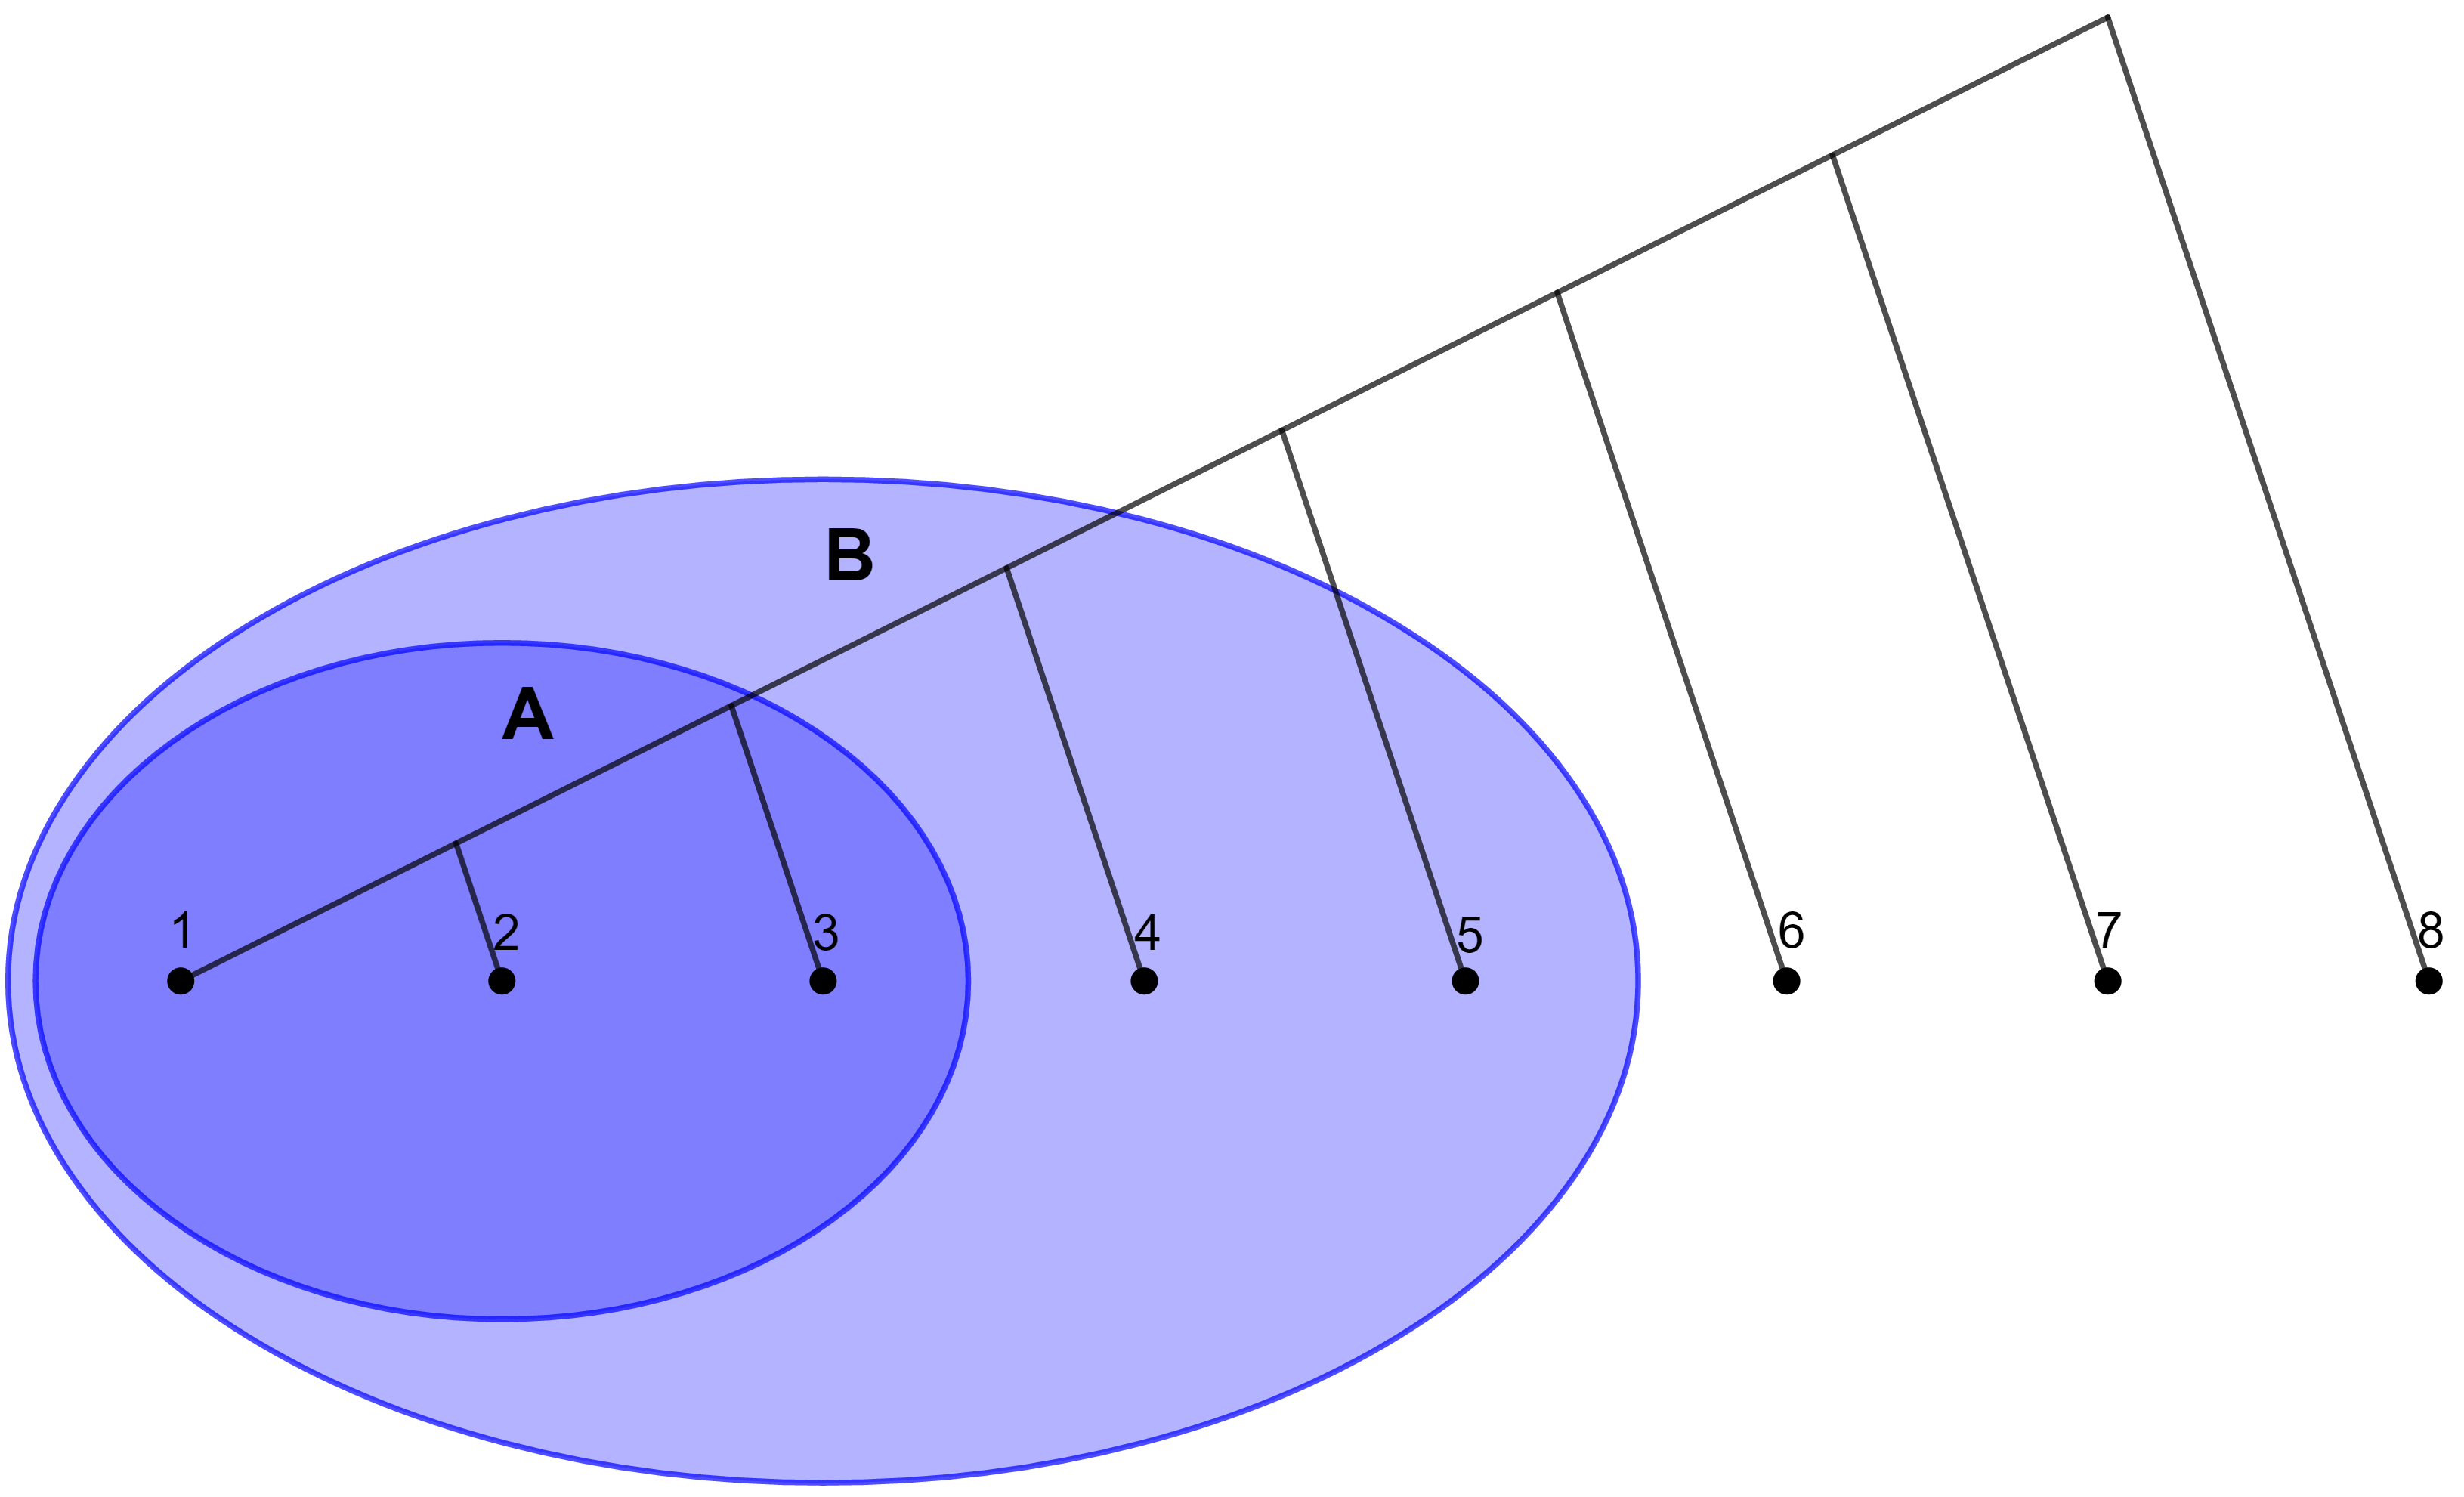
\includegraphics[width=.4\textwidth, margin=0pt 0pt 0pt 1ex,valign=m]{figures/python_tree_example_1.png}}
		& $\Bigg[ \, \bigg[ \, \underbrace{\Big[ \, \overbrace{\big[ \, [ \, [ 1 ], [ 2 ] \, ], [ 3 ] \, \big]}^{A}, [ 4 ] \, ], [ 5 ] \, \Big]}_{8}, [ 6 ] \, ], [ 7 ] \, \bigg], [ 8 ] \, \Bigg] $\\
		\cmidrule(r){1-1}\cmidrule(l){2-2} 
		{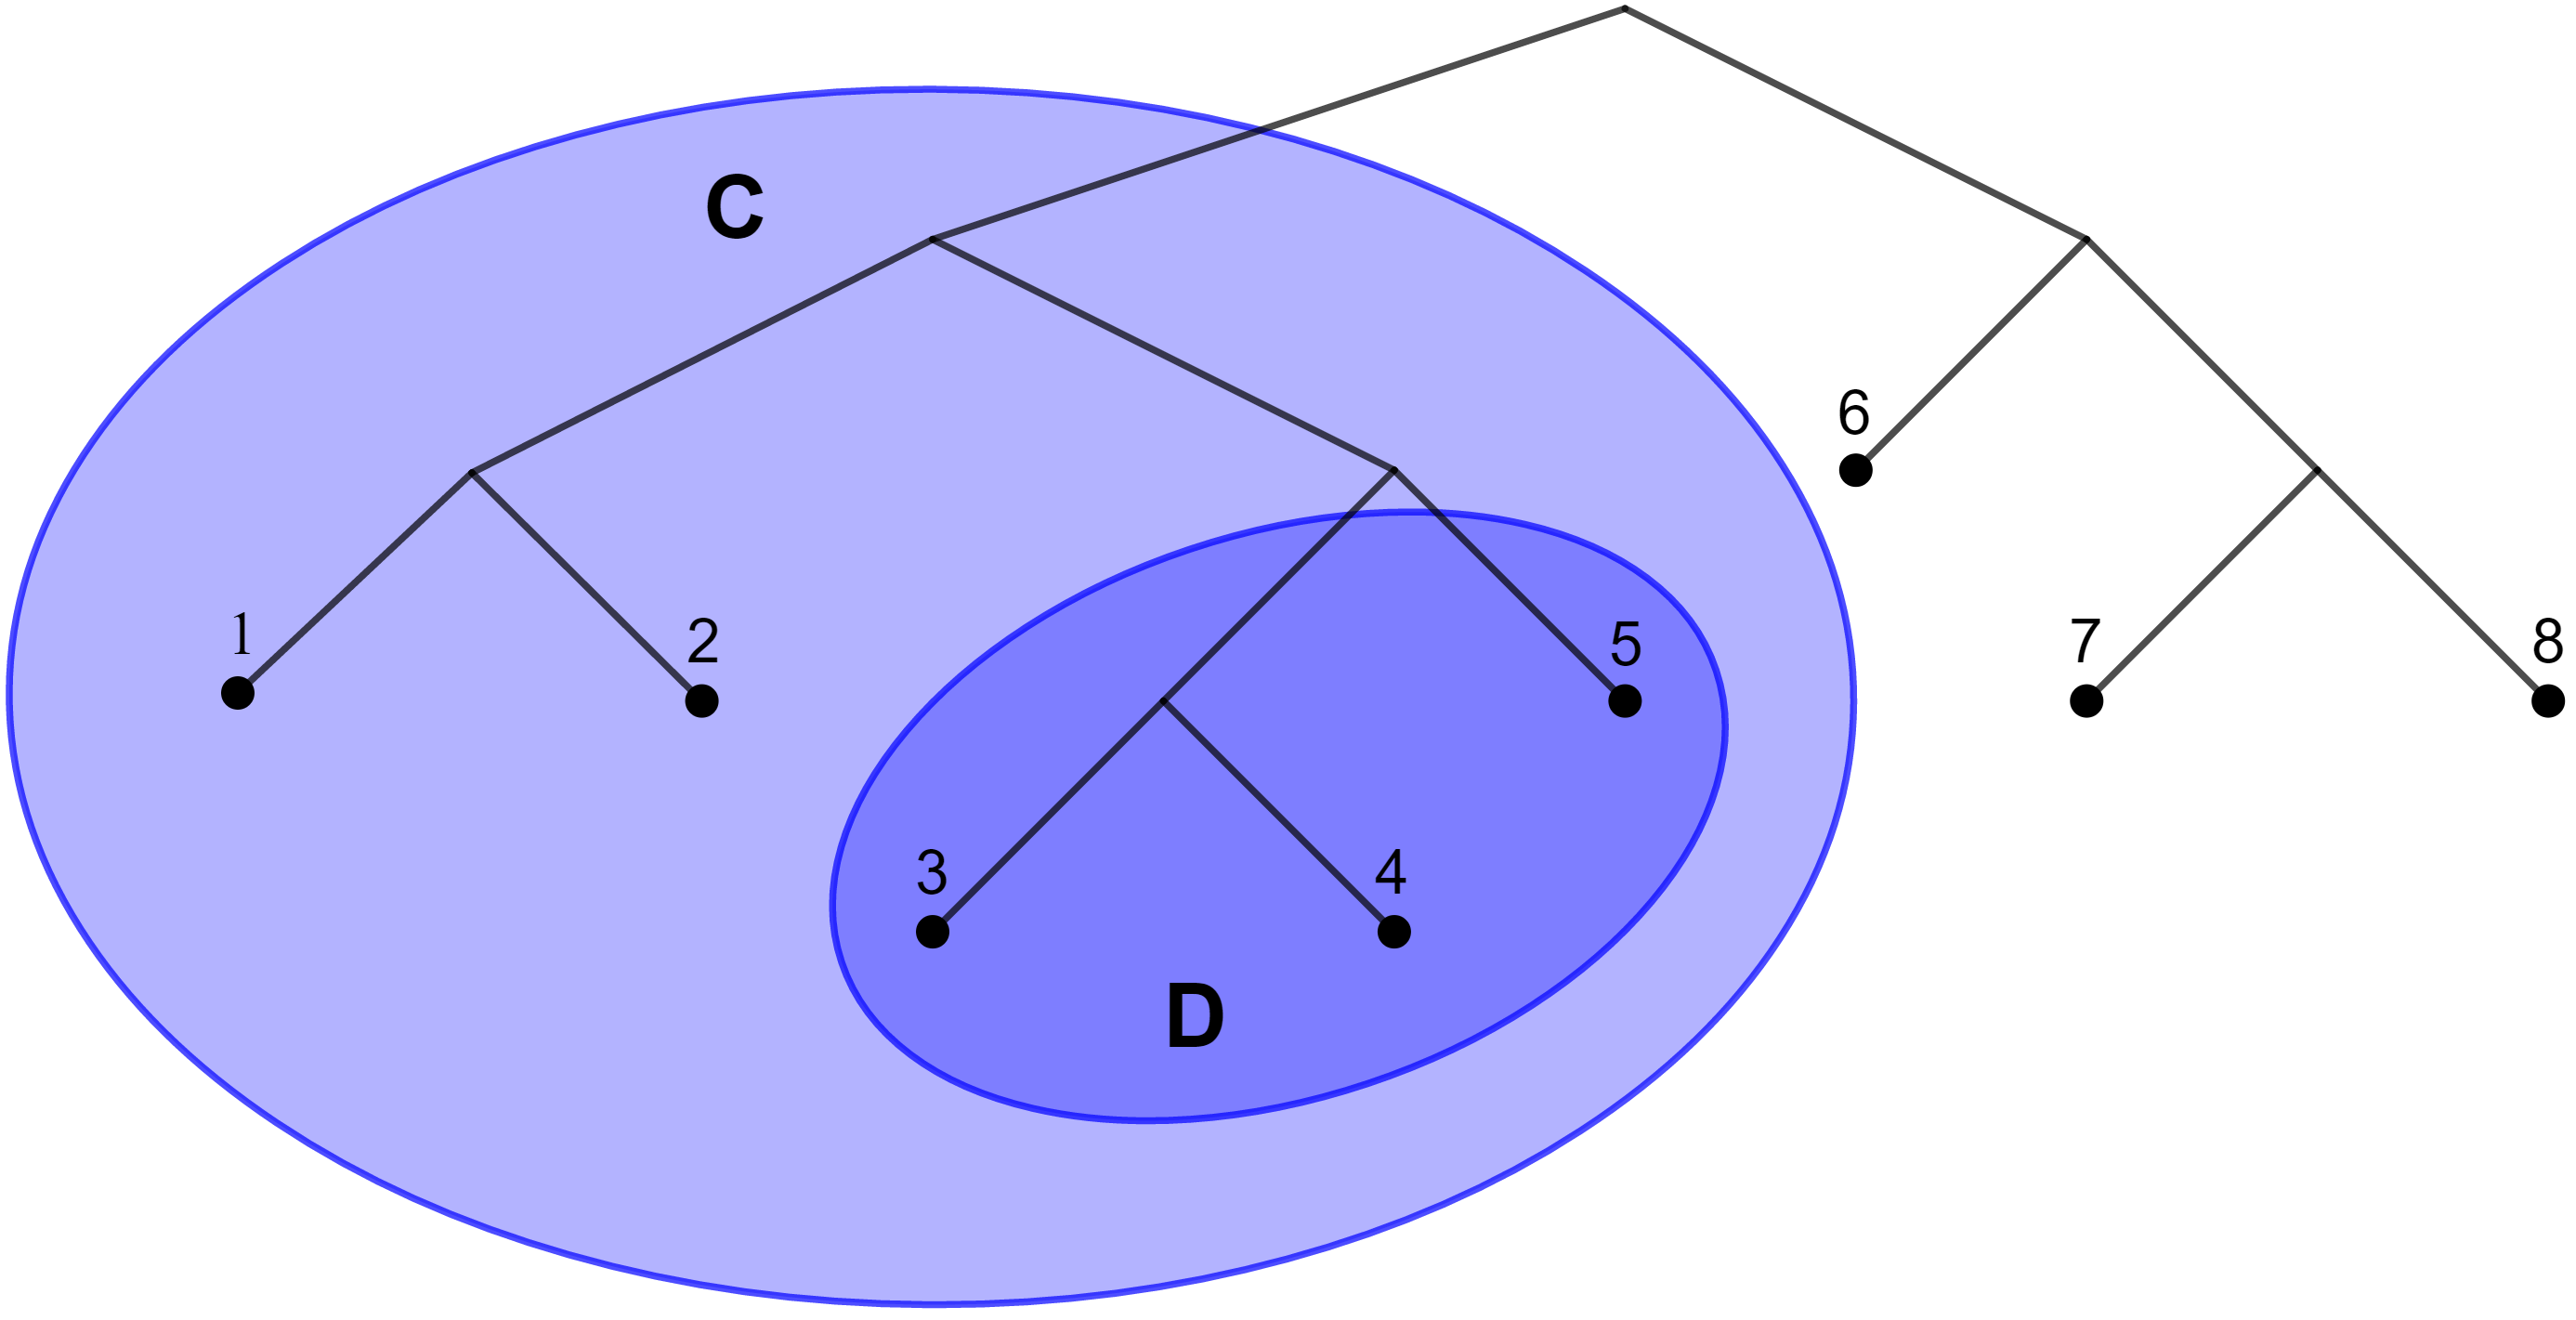
\includegraphics[width=.4\textwidth, margin=0pt 0pt 0pt 1ex,valign=m]{figures/python_tree_example_2.png}}
		& $\Bigg[ \, \underbrace{\bigg[ \, \Big[ \, [ 1 ], [ 2 ] \, \Big], \overbrace{\Big[ \, \big[ \, [ 3 ], [ 4 ] \, \big], [ 5 ] \, \Big]}^{D} \, \bigg]}_{C}, \bigg[ \, [ 6 ], \Big[ \, [ 7 ], [ 8 ] \, \Big]  \, \bigg] \, \Bigg]$\\
		\cmidrule(r){1-1}\cmidrule(l){2-2} 
		{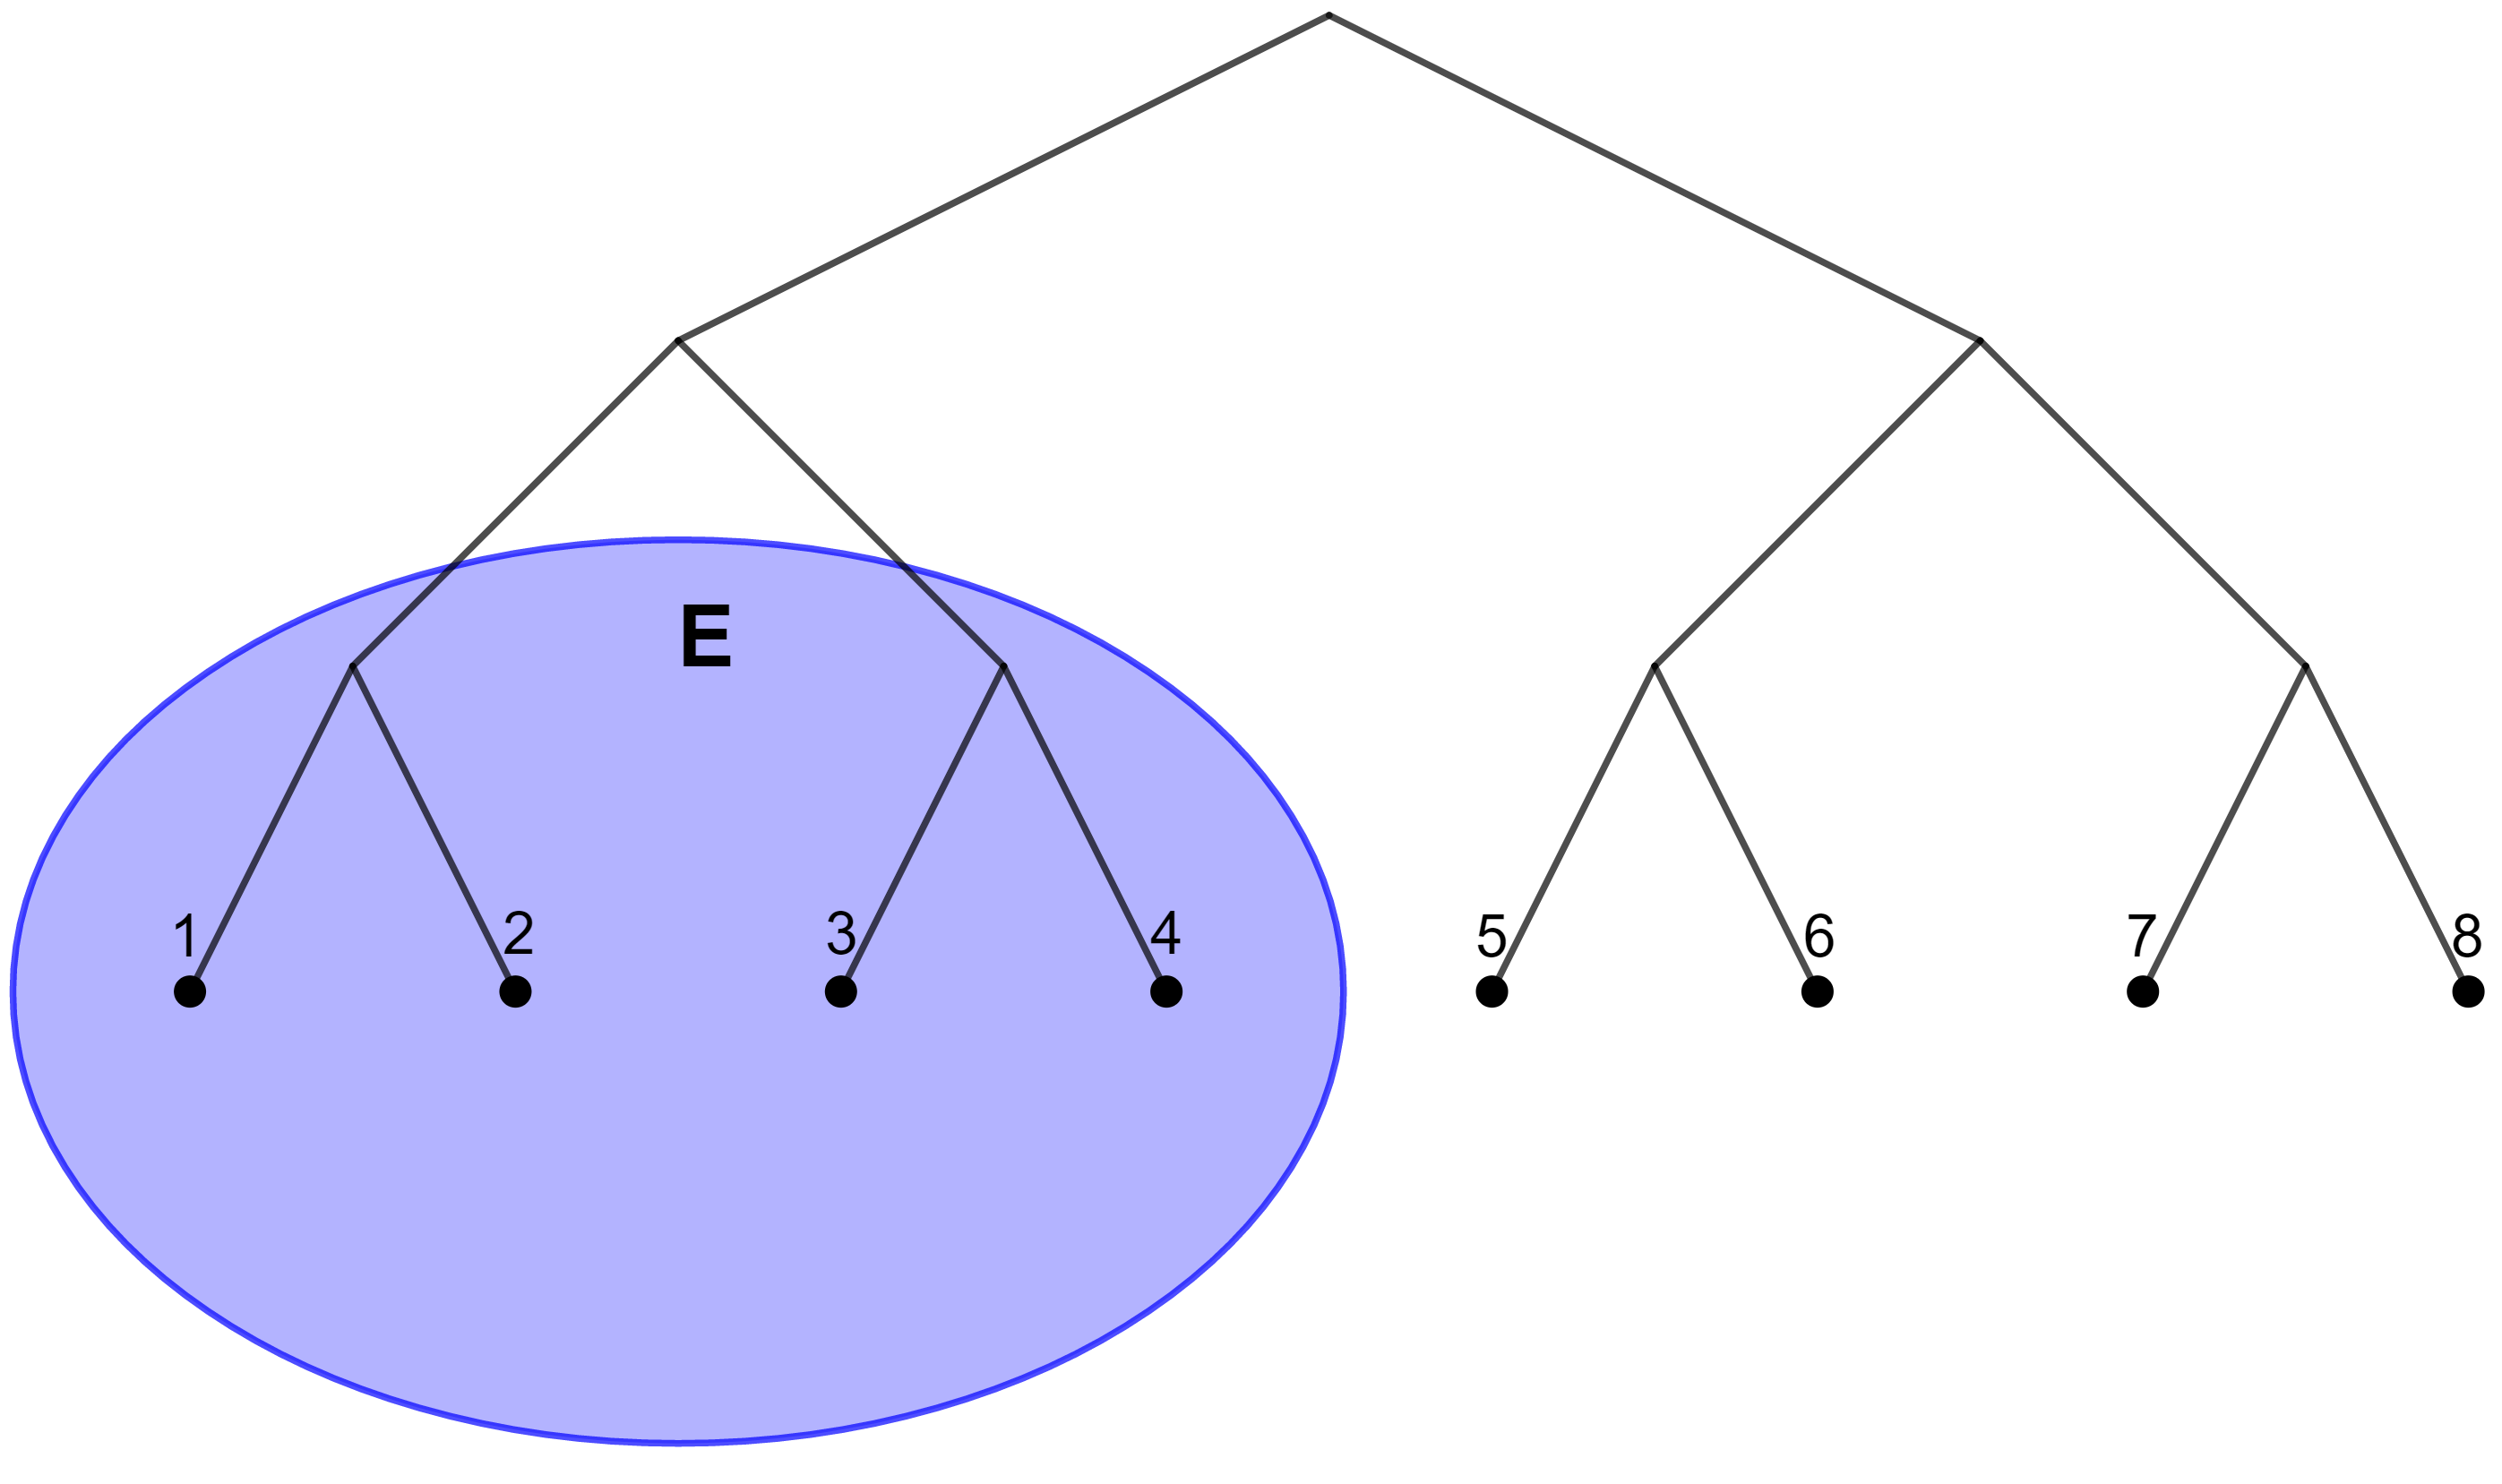
\includegraphics[width=.4\textwidth, margin=0pt 0pt 0pt 1ex,valign=m]{figures/python_tree_example_3.png}}
		& $\Bigg[ \, \underbrace{\bigg[ \, \Big[ \, [ 1 ], [ 2 ] \, \Big], \Big[ \, [ 3 ], [ 4 ] \, \Big] \, \bigg]}_{E}, \bigg[ \, \Big[ \, [ 5 ], [ 6 ] \, \Big], \Big[ \, [ 7 ], [ 8 ] \, \Big] \, \bigg] \, \Bigg]$\\
		
	\end{tabular}
\end{table}

\subsection{Distance Function}
The generalized Robinson-Foulds allows us to choose different distance measures. But since we have to compare our results with the tree edit distance, we need to choose a distance that counts wrong leaves. Therefore we stick with the introduced Robinson-Jaccard metric. We will compute the distances between trees with different values for the constant $k$. Thus we may see a pattern.

\section{Implementation Details}
We based our implementations of both the generalized Robinson-Foulds distance and the tree edit distance on the data structure used in an implementation of Shasha and Zhangs algorithm~\cite{Hen} introduced in Section~\ref{sec:saz}. For computing the generalized Robinson-Foulds distance we extended the data structure \textit{Node} of the above mentioned git repository to include the following functions:
\lstinputlisting[language=Python, caption=Scratch of the class ExtendedNode, label=lst:ExtNode]{figures/extended_node.py}
We based the computation of the generalized Robinson Foulds distance on the linear program introduced in Theorem~\ref{thm:gRF_LP}. We used a widely known, open-source library for linear programms within python, the PuLP- package. \\
Using this package enables us to create an instance of the LP-problem defined in~\ref{thm:gRF_LP} very easily. We start by definining the problem to be a binary LP and by initializing the decision variables $x_{i,j}$. For creating the restrictions we have to loop over all combinations of non-trivial clades in  $\mathcal{C}^*(T_1)$ and $\mathcal{C}^*(T_2)$ and calculate the value $\omega(C_i,C_j')$. Then we formulate the easy restriction from Inequalities~(\ref{eq:V_1}),(\ref{eq:V_2}). Last but not least we compute the set $\mathcal{I}$ to contain any possible combination of invalid edge combinations and add these combinations to the set of restrictions of the LP instance.

\section{Results}
As mentioned above we used the Jaccard metric to calculate the distance between sets of clusters. We used $k \in \{1,2,4,8,16,64\}$ and saw a pattern: Not only is the distance directly proportional to the value of $k$, but the overall distance tends to the standard Robinson Foulds distance very quickly as $k$ increases. \\
Furthermore, without regarding the quality of the results, we realized that the running time is a big problem for this approach. In Lemma~\ref{lem:numberOfRestrictions} we saw that the number of restrictions increases at a rate of (at least) $n^2\log^2(n)$. This leads to a huge ILP even for small trees with only $24$ leaves. Handling such instances with $24$ leaves on both trees already took my computer $500$ seconds. Increasing the number of leaves to $32$ on each tree leads to a running time of about $3100$ seconds. It already takes $22$ seconds to create the LP instance, however one has to be very patient to wait for a solution.\\
It is possible that more evolved linear programming packages solve these problems more efficiently. We tried to use Gurobi for comparison to the running time, but unfortunately this trial mainly delivered errors during the installation. It is possible, that a more advanced package like Gurobi would solve the LP instance faster, nevertheless, this approach doesn't seem to bring fast solutions for big problems as the number of restrictions increases extremely fast.
\chapter{Implementation Generalized Robinson Foulds}
\section{Preparation and Overview}
\section{Implementation Details}
\section{Results}
\chapter{Conclusion}
This thesis tries to give a short insight into a large and widely ranged topic of comparing trees.

First we give some basic notations and definitions since the language varies greatly between different papers and authors. 

The first idea of comparing trees is the tree edit distance. Editing one tree into the other, by using simple operations such as deleting, inserting and relabelling step by step, is one intuitive way of comparing trees. Every operation is associated with some costs. The task is to find a sequence of editing operations of minimal costs, that alters both trees to become the same. There are simple algorithms using a dynamic programming approach that can compute the tree edit distance to optimality. We start with Shasha and Zhang~\cite{SasAndZha}, who used a trivial decomposition strategy which guides an iterative, recursive algorithm which always compares the rightmost subtrees. Then we present the algorithm of Klein~\cite{Kle} and the algorithm of Demaine et al.~\cite{Dem}. These algorithms involve more sophisticated decomposition strategies which take into account the sizes of the investigated subtrees. Demaine et al. provided a lower bound on the running time for computing the tree edit distance with a dynamic programming approach. Furthermore they proved that their algorithm satisfies this bound, making it optimal among all algorithms with a dynamic programming approach. 

Moreover in chapter $4$ we proceed with the so called flexible tree matching. Here the idea is that one may relax the restrictions of ancestry and sibling groups. Instead of forbidding such violations we just have to pay a fine for any occurrence. Unfortunately finding the flexible tree edit distance is a strongly $\mathcal{NP}$-complete problem. Nevertheless we present a model for approximation heuristics. Kumar et al.~\cite{Kum} provided a Monte Carlo algorithm to compute an approximation of the flexible tree matching.

In chapter $5$ we take a look at a widely used measure, the Robinson-Foulds metric. Working on the same set of taxa (or leaves), we want to know how many clades are present in exactly one of the two investigated trees. We discuss its advantages and disadvantages and generalize it to make it more applicable using more evolved cost functions. However, we still end up with a $\mathcal{NP}$-complete problem of finding a minimum cost arboreal matching between the sets of non-trivial clades.


%\appendix                       %% closes main document, appendix follows until end; only available in book-classes
%\addpart*{Appendix}             %% adding Appendix to tableofcontents
\begin{thebibliography}{99}

\bibitem{Apo}
  Apostolico A., Galil Z.,
  \textit{Pattern matching algorithms},
  Oxford University Press,
  1997
  
\bibitem{Bil}
  Bille P,
  \textit{A survey on tree edit distance and related problems},
  Theoretical computer science,
  2005,
  217–-239
  
\bibitem{Boe}
  Böcker S., Canzar S., Klau G.,
  \textit{The Generalized Robinson-Foulds Metric},
  International Workshop on Algorithms in Bioinformatics,
  2013,
  156–-169,
  
\bibitem{Bog}
  Bogdanowicz D., Giaro K. and Wróbel B.,
  \textit{TreeCmp: Comparison of Trees in Polynomial Time},
  Evolutionary Bioinformatics 8,
  2012,
  475--487
   
\bibitem{Che}
  Chen W.
  \textit{New algorithm for ordered tree-to-tree correction problem},
  J. Algor. 40,
  2001,
  135--158
  
\bibitem{Dem}
  Demaine E. D., Mozes S., Rossmann B. and Weimann O.,
  \textit{An Optimal Decomposition Algorithm for Tree Edit Distance},
  ICALP'07 Proceedings of the 34th international conference on Automata, Languages and Programming,
  2007,
  146--157

\bibitem{DulAndTou}
  Dulucq S. and Touzet H.,
  \textit{Analysis of tree edit distance algorithms},
  Proceedings of the 14th Annual Symposium on Combinatorial Pattern Matching (CPM),
  2003,
  83--95
  
\bibitem{Git}
  Andritsch C.,
  \textit{Master Thesis},
  Github Repository,
  \url{https://github.com/bananajoe/masters_thesis},
  2019
  
\bibitem{Har}
  Harel D. and Tarjan R. E.,
  \textit{Fast algorithms for finding nearest common ancestors},
  SIAM J. Comput. 13, 2,
  1984,
  338--355
  
\bibitem{Hen}
  Tim Henderson
  \textit{Zhang-Shasha: Tree edit distance in Python},
  Github Repository,
  \url{https://github.com/timtadh/zhang-shasha},
  2019
  
\bibitem{Kle}
  Klein P. N.,
  \textit{Computing the edit-distance between unrooted trees}, 
  Proceedings of the 6th Annual European Symosium on Algorithms (ESA),
  1998,
  91--102
  
\bibitem{Kum}
  Kumar R., Talton J., Ahmad S., Roughgarden T., Klemmer S.,
  \textit{Flexible Tree Matching},
  Proceedings of the 22nd International Joint Conference on Artificial Intelligence,
  2011,
  
\bibitem{Moo}
  Moore P.,
  \textit{Strucural motifs in RNA},
  Ann. Rev. Biochem 68,
  1999,
  287--300
  
\bibitem{SasAndZha}
  Sasha D. and Zhang K.,
  \textit{Simple fast for editin distance between trees and related problems},
  SIAM J. Comput. 18, 6,
  1989,
  1245--1262
  
\bibitem{Tai}
  Tai K.,
  \textit{The tree-to-tree correction problem},
  J. Assoc. Comp. Mach. 26,
  1979,
  422--433
  
\bibitem{Val}
  Valiente G.,
  \textit{Algorithms on Trees and Graphs},
  Springer-Verlag,
  2002,
  
\bibitem{Wag}
  Wagner R. and Fischer M. J.,
  \textit{The string-to-string correction problem},
  J. ACM 21, 1,
  1974,
  168--173
  
\end{thebibliography}  
\end{spacing}

\end{document}
